% +------------------------------------+
% |   Generated by www.docx2latex.com  |
% |   Version: 2.0.0                   |
% +------------------------------------+

\documentclass[11pt]{book}

\usepackage{caption}
\usepackage{fancyhdr}
\usepackage{float}
\usepackage[T1]{fontenc}
\usepackage{graphicx}
\usepackage[utf8]{inputenc}
\usepackage{subcaption}
\usepackage[normalem]{ulem}
\usepackage[paperheight=29.69cm,paperwidth=21.01cm,left=2.54cm,right=2.54cm,top=2.54cm,bottom=2.54cm]{geometry}
\usepackage[hidelinks]{hyperref}


\setlength\parindent{0pt}
\renewcommand{\arraystretch}{1.3}\lfoot{\thepage}



\title{DiRT: Distributed Robotic Tools for Spatial Timber Assembly with Integral Timber Joints}

\begin{document}
\maketitle

\chapter{Title}

\chapter{Abstract}

This thesis investigates the potential of distributed robotics systems in automating the assembly of timber structures, addressing the challenges of large-scale spatial manipulation and tight-fitting timber joint assembly, which are highly relevant for timber construction.

Leveraging the highly automated process of machining timber parts using automatic joinery machines, the thesis investigates the next knowledge gap in the design-to-production workflow - automatic spatial assembly. Using timber frame structures with integral timber joints as a starting point, this thesis proposed a new fabrication system using distributed robotic tools (DiRT) in collaboration with industrial robotic arms. The crucial breakthrough is the modular and remote operation nature of the tools, allowing the system to assemble a wide variety of timber joints and complex structures.

This thesis also investigated an integrated design workflow. Design validation is identified as a critical aspect of the automated assembly process. This research proposes a practical three-tier validation process to evaluate a design, with quick feasibility feedback provided to the designer during the design process. It takes into consideration geometrical conflicts, robot limitations and tool setup to provide visual feedback on various problems to the designer. 

The research provides a proof-of-concept through the development of three full-scale timber frame demonstrators, each assembled using a single robotic arm and a set of custom-designed distributed assembly tools. The assembly tools include robotic clamps and screwdrivers for different types of lap joints, including planar and non-planar varieties. The findings showcased a viable method to assemble timber structures, mitigating well-known problems such as accumulated assembly error and instability during construction. The results also identified key challenges that are limiting the system efficiency, accuracy, reliability and success rate for the automated process, as well as discovering new opportunities for future research. These opportunities include establishing a generalizable DiRT assembly system, and expanding the range of joint types and building components that can be assembled.

The thesis contributes software tools and system design patterns that are generalizable and reusable within the broader digital fabrication and construction automation community. For example, software for remote robot operation and synchronisation; Data structures and algorithms for robotically assembled structures; Methods for automating parsing designs into robotic programmes; and Task and motion planning techniques for assembly problems.

Ultimately, this research contributes to ongoing efforts to harness the potential of robotics for creating more efficient and sustainable timber construction processes. Paving the way for the widespread adoption of automated construction processes within the architectural industry.


\newpage

\chapter{Table of Contents}


%%%%%%%%%%%%  This Produces Table Of Contents  %%%%%%%%%%%%
\tableofcontents
\vspace{1\baselineskip}

\newpage

\chapter{Introduction}

The advancement of technology has opened new avenues for innovation in construction. The use of robots in the assembly of timber structures presents a new frontier in this field. This interdisciplinary PhD thesis focuses on the integration of industrial robots and distributed robotic tools (DiRT) for the automatic assembly of timber structures. Specifically, timber frame structures with integral timber joints. 

Despite the potential benefits that automation could bring to the construction industry, the necessary technology to achieve this goal remains unknown. The objective of this thesis is to embark on a journey of discovery and innovation that will contribute to the advancement of knowledge in the field. By combining interdisciplinary approaches from timber construction, computational design and robotics, this research will provide insights into the technical and operational aspects of the automatic assembly process, as well as its potential benefits and challenges. Through the development of novel solutions and empirical construction experiments, this PhD thesis aspires to shape the future of construction and contribute to the interdisciplinary field of digital fabrication, between architecture, construction and robotics.

\section{Timber Frame Construction}

Timber construction has been used historically in many cultures with an ample supply of trees. Timber is a remarkable construction material because of its very high strength-to-weight ratio. It can withstand tension and compression, making it suitable for different structural roles. Moreover, timber can naturally reach lengths of many metres, which provides tall columns and long beams for the construction of architectural structures at various scales. Historically, many types of construction methods have been developed. The focus of this thesis is timber frame construction which refers to a range of timber construction methods used as early as the 12th century until the early 20th century \href{https://www.zotero.org/google-docs/?j9TO86}{(Sobon $\&$ Schroeder, 1984)}.

\subsection{Defining Characteristics}

We can understand timber frame construction as a set of techniques that have evolved over time. Carpenters have experimented with different joint designs, structural arrangements and methods to frame walls, floors and roofs. While these techniques evolved independently in different civilisations, similar material behaviour (e.g. anisotropicity of wood, prone to decay) and similar design goals (e.g. weather protection) resulted in many similarities between them \href{https://www.zotero.org/google-docs/?RgN7ZN}{(Zwerger, 2012)}. While there are still differences between regional practices (caused by regional timber species, weather, local culture and ornamental preferences), the type of timber construction that dominated the pre-industrial era (especially in Europe, North America, and Japan) share similar defining characteristics: (1) Large timber sizes, (2) integral timber joints, and (3) post-and-beam framing. 

These characteristics make timber frame construction ideal for studying automatic assembly. As such, this thesis is not referring to the timber frame construction of a specific location or time period, but rather to the general use of these three defining characteristics of timber frame construction.

\subsubsection{Large Timber Size}

The first defining characteristic of timber frame construction is large timber sizes. Historically, this is the result of using a whole harvested tree trunk as a structural member instead of laboriously cutting them into smaller pieces. It was only after the industrialisation of sawmills that timber could be efficiently cut into smaller dimensions. Around the same time, the depletion of large trees in Europe and America prompted the more contemporary invention of stick framing construction (i.e. balloon framing and platform framing) that uses dimensional lumber (e.g. 2x4 inch ``two-by-four" studs). Later as timber glue technology improved, the use of glue-laminated timber (glulam), laminated veneer lumber (LVL) and other engineered timber products began to appear and allowed the manufacturing and use of large timber elements again. In this thesis, the assembly of both solid timber and engineered timber is investigated. The nominal size being used is 100mm x 100mm square profile \textit{(see \underline{4.1.3 Scope for Initial Development Round})} 

\subsubsection{Integral Timber Joints}

The second defining characteristic in timber frame construction is the use of integral timber joints (ITJ), where the jointing geometry is carved into the material.\textbf{ }Structural load is transmitted from element to element directly through contact pressure over the mating surfaces of the joint. The design of these joints has been refined empirically throughout history, converging into specialised designs according to which structural elements they are connecting \href{https://www.zotero.org/google-docs/?BttU29}{(Jack Sobon, 2014)}. It is common for a joint to serve multiple purposes and thus withstands different types of loads, such as self-weight and live forces. Different ‘geometrical features’ can therefore be incorporated into the connection to meet different force conditions. For example, a lap joint for a floor joist can be combined with a dovetail feature to provide tension resistance. These joints are typically dry-fitted \textit{(footnote: because historical glue technology could not withstand structural forces) }and held in place due to interlocking geometry and gravity. Additionally, it is possible to include metal components in integral timber joints. This is more common in contemporary design, where metal screws, dowels and tie rods are used to improve joint capacity or to reduce the need to cut complicated joinery. For the purpose of studying automatic assembly, integral timber joints provide a unique advantage because they can be prefabricated with high accuracy \textit{(see \underline{1.1.2.1 Automatic machining of parametric timber joints})} and are quick to install. In this thesis, the assembly of dry-fitted joints both with and without fasteners is explored.

As of today, there is no single consensus in the nomenclature of timber joints as different cultures have historically named their joints using different methods \href{https://www.zotero.org/google-docs/?WvT4uQ}{(Sato $\&$ Nakahara, 1995; Seike, 1977; Sumiyoshi $\&$ Matsui, 1991)}. The first naming convention (commonly used in American and European traditions) is based on the location of the joint and the structural elements it connects to, for example, ‘floor joist joint’ or ‘tying joint below plate’. The second naming convention is based on the joint's geometrical features, for example, ‘dovetail joint’ or ‘scarf lap joint’. Some unique joint designs could also be named according to the use in a famous building. For example, Osaka-jo-otemon-hikae-bashira-tsugite refers to Osaka Castle-Otemon Gate's pillar splice. For the purpose of studying assembly problems, this thesis proposes the use of a different convention that is based on the assembly direction related to the joint \textit{(see \underline{Section 4.2.1 Lap Joint Classification by Assembly Direction)}}.

The photo below shows timber frame components being assembled on the ground. Notice the use of large timber sizes and integral timber joints. 

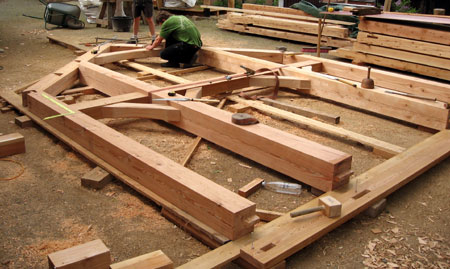
\includegraphics[width=11.91cm,height=7.12cm]{./images/image5.jpg} \\ {\footnotesize (Credits: CC AS 4.0 Licence photo by Georg Hefter - Traditionelles Fachwerk und Timberframe im Vergleich auf georghefter.de)\par}

\subsubsection{Post and Beam Structure}

The third defining characteristic of timber frame construction is post-and-beam structural framing \href{https://www.zotero.org/google-docs/?KMFAqo}{(Jack Sobon, 2014; Sobon $\&$ Schroeder, 1984)}. The use of large timber sizes in timber frame structures allows them to be strong enough without the use of continuous load-bearing walls. The main benefit is the flexible arrangement of floors and walls to suit different architectural programmes. 

On the other hand, integral timber joints are generally weak in rotational stiffness, causing the joints to behave kinematically. Therefore, diagonal bracing is often introduced to fully or partially triangulate the structure to improve structural stiffness. Being limited by the joint design, these bracings function primarily in compression. It is, therefore, common to design the bracings in complementary pairs to resist dynamic wind loads coming from opposing directions. While some architectural designs may find the intrusion of diagonal bracings obtrusive to usable space, these diagonal bracings are highlighted on the facade as ornamentation in half timber designs \href{https://www.zotero.org/google-docs/?NgmBHM}{(Gerner, 1979; Skinner, 2007)}. In this thesis, the demonstration structures are designed with similar structural principles, specifically the use of structural triangulation in the design offered unique stability advantages during the robotic construction process \textit{(see \underline{7.1.1 Deformation-Awareness and Error Correction by Triangulation} and \underline{7.5.2.6 Global Correction Approach})}.

The image below shows an example of a half-timber style timber frame house in Soest, Germany. Notice the exposed diagonal elements on the facade.

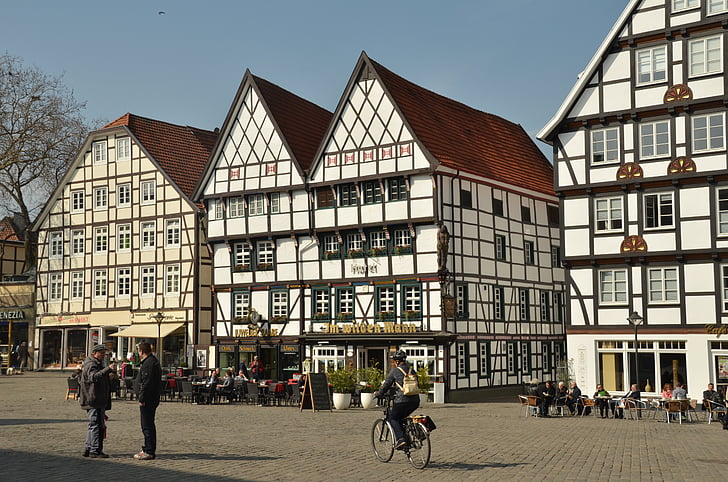
\includegraphics[width=15.92cm,height=10.55cm]{./images/image9.jpg}{\footnotesize (Credits: Licence-free photo, retrieved from https://www.hippopx.com/en/germany-soest-architecture-timber-framed-half-timbered-house-square-city-402214 , n.d.)\par}

\subsection{Current Practice of Timber Frame Construction}

Timber frame construction was once the dominant building method, but it gradually declined in popularity during the 19th and 20th centuries. The advent of industrialization and mass production led to the availability of cheaper building materials such as steel and concrete, which were faster and easier to use. Even within the timber construction sector, newer construction methods that use dimensioned lumber, glulam, LVL, and cross laminated timber (CLT) have replaced timber frame construction. However, in recent years, as more people are aware of the environmental benefits of wood construction, interest in timber frame construction is increasing again as an alternative way to construct with timber. 

Advancements in engineering and design, as well as increased availability of sustainably sourced timber, have helped to make timber frame construction a more viable option for modern building projects. Timber frame components can be prefabricated off-site, which can reduce construction time and costs while also minimising waste and environmental impact. The use of dry-fitted integral timber joints reduces the number of fasteners and components involved, meaning less metal consumption and quicker installation on-site. Finally, timber frame structures can be aesthetically pleasing as they often expose the beautiful timber material and reveal the structural load paths. When the joint details are exposed, they can evoke a feeling of tradition and craftsmanship and are often well-appreciated by those who inhabit the building.

\subsubsection{Automatic Machining of Timber Joints}

Between the years of decline and its recent resurgence, a number of technological improvements have made timber frame construction more efficient and competitive. One of the major advancements has been the use of automatic joinery machines for carving integral timber joints. Traditionally crafted with hand tools, these joints were labour-intensive and required highly skilled craftsmen that could work precisely.\footnote{ The task of marking and setting out was considered the most critical and is often performed by the master carpenter. Other carpenters would prepare materials and carve joints using hand tools such as saws, planes, chisels, and drills.}\textit{ }Since the invention of automatic joinery machines, the production of timber joints has become highly automatic \href{https://www.zotero.org/google-docs/?1lvKCf}{(Hans Hundegger AG, 2023)}. These machines often feature interchangeable cutting tools and can create many types of joints at the beam ends and along its length. Today, the machining of timber joints is very mature and efficient. The automatic joinery machines are controlled by computer numeric control (CNC) technology and can follow a digital program to create timber joints of different designs at different positions. The program can be quickly changed to create different timber elements used for an entire building. \textit{(see \underline{1.2.4 Programming Digital Fabrication Machines} for details about control and programming)}

This thesis capitalises on the accuracy and prefabrication efficiency provided by the automatic joinery machines. Accurate parts are highly advantageous for robotic automatic assembly because they ensure accurate manipulation and precise integration. By using prefabricated timber parts with accurately machined integral timber joints, this thesis aims to create a highly automated assembly process, reducing the manual labour needed for adjustment and adaptation. 

\subsubsection{Assembly by Carpenters}

Although the production of timber frame components is automated, the assembly of the structure is still predominantly manual \href{https://www.zotero.org/google-docs/?mMONEv}{(Willmann, Gramazio, et al., 2016)}. It usually takes a team of carpenters to assemble a timber structure.

Timber frame structures are almost always assembled on-site due to the nature of their post-and-beam structural system, which favours long and unbroken elements. This means that pre-assembling multiple elements off-site, is not practical because it will result in assemblies that are too big for transportation. 

Below is a summary of the tasks that carpenters perform during the assembly of a timber frame structure, focusing on the structural elements:

\begin{itemize}
	\item \textbf{Sorting timber parts - }Prefabricated timber parts are typically delivered on-site in bundles that correspond to different assembly stages. Many of the components are geometrically unique because of the layout of the joints. Carpenters must identify the correct location for each element based on label and markings on the parts and sort them according to the assembly sequence.

	\item \textbf{Manipulating timber parts spatially - }Post, beam and diagonal bracings are assembled in different spatial (3D) orientations. Carpenters must identify and orient the parts correctly when bringing them to their assembly location.

	\item \textbf{Applying forces - }Because of contact friction and deformation, carpenters may need to apply force to the joints using hand tools. They may use common generic tools such as mallets and screwdrivers (pulling with a screw), or specialise tools such as ratcheting joint pullers. 

	\item \textbf{Aligning mating joints -} Multiple carpenters are often required at every mating joint. They may have to push or pull the already-assembled elements for alignment. 

	\item \textbf{Synchronous Assembly - }During the closure of the joints, the carpenters also ensure parallel and synchronous motion to avoid jamming.

	\item \textbf{Adjusting timber joints - }If a timber part does not fit. Carpenters can remove material or shim gaps. These types of problems are rare with CNC fabricated parts, but can sometimes occur due to poor machining tolerance, design error, machine-programming error, and shrinkage or expansion after machining.

	\item \textbf{Placing fasteners} - Some contemporary joint designs include screws, nails, or dowels.

\end{itemize}
These tasks are the focus of the automated assembly process pursued in this thesis. The challenges of each task are analysed and presented in the next chapter \textit{(see \underline{2.1 Mechanical Challenges)}}.

\subsection{New Opportunities for Timber Frame Construction}

Compared to other newly developed construction methods with a higher degree of prefabrication, the on-site timber frame construction is less economically competitive. For example, modular floor and wall construction allow more components to be assembled off-site (e.g. insulation, windows, doors), which reduces the time and cost associated with on-site work. Volumetric prefabrication (e.g. modular timber construction), which pre-assembled an entire room, further allows the installation of wiring, plumbing, and interior finishes in a factory \href{https://www.zotero.org/google-docs/?zzjLzT}{(Adel et al., 2018)}. 

Despite the lack of prefabrication advantages, timber frame construction enjoys greater design freedom because there are fewer transportation constraints when moving linear timber elements than moving a preassembled room-sized timber module. This freedom is essential in creating large-span structures or shell structures where sub-assemblies cannot be effectively transported. In addition, latest timber frame designs have already been able to integrate contemporary building requirements such as plumbing, electrical wiring and insulation that meets building codes \href{https://www.zotero.org/google-docs/?zzM1PB}{(Benson, 1988)}. Therefore, the exploration of automatic assembly for timber frame structures could potentially keep these benefits without the associated penalty of on-site manual work.

\section{Architectural Design to Production}

In recent years, the fields of architecture and construction have seen a growing interest in automating various stages of the design and production process. This trend is being driven by the potential benefits of automation, which include increased efficiency, higher precision, and improved quality control. Automation can also help to reduce labour costs, minimise waste, and improve safety on construction sites. While automation has already become common in the manufacturing industry, its adoption in architecture and construction has been slower due to the unique challenges and complexities in the construction sector. Most commercialised examples are limited to prefabrication of small or planar architectural components while only a handful of research projects have attempted to use robotics for structural scale spatial assembly. Therefore, this thesis aims to expand knowledge in this area, starting with the assembly of timber frame structures.

This section will present a brief history of how the timber construction industry transitioned towards digital design and automated production, leading to the current state of the art practices. It is an important starting point to understand whether the assembly process will also undergo such a transition. 

\subsection{Automation from Manufacturing to Construction}

The beginning of automation started with the manufacturing industry. It involves the use of machinery or computer systems to perform tasks that would otherwise be done by human labour. Without going into details, it typically involves the use of sensors, actuators and control systems to reduce or eliminate the need for human intervention \href{https://www.zotero.org/google-docs/?WadYaU}{(Nof, 2009)}. It has become a widely adopted practice in the manufacturing industry due to its benefits such as increased efficiency, improved quality, and reduced costs. With automation, the production process can run 24/7, leading to a predictable production schedule and reducing the need for manual labour. 

The successful implementation of automation is closely tied to the design and operation of production machines. Since the beginning of industrial automation, automatic machines have undergone several evolutions that are characterised by their features, modes of operations and benefits. Early automatic machines were mechanical systems that performed repetitive fixed operations. Their motions were often defined mechanically through the use of components such as linkages, cams and conveyor belts. Because of this, their motions cannot be easily modified without changing parts. These machines favour high-volume, low variability products that represent the mass-production paradigm of Industry 2.0\footnote{ The First Industrial Revolution, aka. Industry 1.0, began in the late 18th century where mass production was carried out by machines powered by water and steam.}. While some of the earlier machines still require an operator, later machines would contain control systems that are capable of performing cyclic actions on their own. After the introduction of electricity, the use of logic controllers became more common and allowed the machines to make decisions using sensors and signals. The increased level of autonomy allowed further reduction of operator interventions. This type of automation is a typical defining characteristic of Industry 3.0 \href{https://www.zotero.org/google-docs/?idxPsd}{(Menges, 2015; Yin et al., 2018)}. 

Invented in the 1950s and popularised in the 1960s, Computer Numeric Control (CNC) technology further increased the flexibility of machines, such as the aforementioned automatic joinery machines and industrial robotic arms. The motion of CNC machines are defined through the use of a digital ‘program’ such that their motion can be easily modified when products are changed \href{https://www.zotero.org/google-docs/?zaXN8V}{(Ward, 1959)}. This is often achieved by incorporating a computerised digital control. The ability to change design quickly eventually led to the mass-customisation paradigm of Industry 4.0. In extreme cases, products can even be unique from piece to piece, resulting in the ‘batch size of one’ paradigm \href{https://www.zotero.org/google-docs/?zgkMNk}{(Ward, 1959)}.

The adoption of automatic machines has changed the nature of work from labourers to operators and increasingly towards engineers and programmers \href{https://www.zotero.org/google-docs/?iYzGBf}{(Noble, 1986)}. While this shift may be difficult for workers unable to acquire a new skill set, it improves the general labour working conditions in the longer term \href{https://www.zotero.org/google-docs/?RBFbyp}{(Stromquist, 2019)}. For example, by reducing repetitive manual tasks or avoiding working in dangerous environments. 

\subsubsection{A Factory for Making Buildings}

At a larger scale, the concept of automation can be applied to connect different machines together to autonomously regulate production flow. There are two types of connections involved, the first is physical connections, such as using conveyor belts and robotic arms to move parts between machines. The second is logical connections, such as programmable logic controllers forming complex logic networks. In extreme cases, the term ‘lights-out factory’ or ‘automatic factory’ was used to describe large production facilities that are able to sustain continuous production with very few or infrequent operator involvements \href{https://www.zotero.org/google-docs/?1vGmg1}{(Noble, 1986; Walker, 1957)}. 

Recently, the introduction of large-scale concrete 3D printing technology has brought the automatic factory vision within reach for the architecture and construction community \href{https://www.zotero.org/google-docs/?rmNu2g}{(Ngo et al., 2018)}. While large-scale 3D printing processes are still at the research stage, smaller 3D printers have already achieved full autonomy, allowing users to press a start button and come back later for the completed parts. The idea of a black-box fabrication machine where design information and raw materials are the only input, was hypothesised to be the future mode of production that can make almost anything. \href{https://www.zotero.org/google-docs/?YpV7gl}{(Gershenfeld, 2012; Gershenfeld et al., 2004)}.  

Started in the late 1970s, Japan’s large construction contractors have begun developing robots capable of performing construction tasks. The initial robots were single-task construction robots, designed to perform one specific function, such as finishing concrete, welding, or spray painting \href{https://www.zotero.org/google-docs/?vwNv2H}{(Potter, 2022)}. Starting in the mid-1980s, Japan’s construction robot development shifted away from individual robots, and towards creating an entire robotic construction site \href{https://www.zotero.org/google-docs/?f7fifK}{(Maeda, 2005)}. The process often makes use of a high number of prefabricated components and focuses on improving the speed for the assembly task. Studies have found that the productivity gain is often apparent when constructing a tall and repetitive building. \href{https://www.zotero.org/google-docs/?NRpif9}{(Linner, 2013; Potter, 2022)}. 

While the automated systems seen in Japan are mostly designed for steel and reinforced concrete structures, this thesis studies what it would take for timber construction to achieve a similar level of automation. 

\subsection{Automatic Assembly in Timber Construction}

In recent years, interest in exploring automatic assembly for timber construction has grown. This was driven by the potential for increased efficiency, precision, and sustainability. Despite the advancements in fabrication techniques, particularly with the advent of CNC technology, the assembly process still presents challenges that industry professionals and researchers are working to address \href{https://www.zotero.org/google-docs/?VCZ0h4}{(Willmann, Gramazio, et al., 2016)}.

In the industry, the advancement was mainly focused on the assembly of flat-stackable prefabricated parts, such as light-framed timber floors and walls. Companies like Biesse, Homag, and Weinmann have been developing advanced machinery and automated solutions for timber processing and assembly \href{https://www.zotero.org/google-docs/?Ii4M5y}{(Koo et al., 2021)}. These systems are often large-scale installations similar to a manufacturing production line and are custom engineered for a specific factory. The entire system can include separate material processing stations, such as cutting and joinery machines and for linear timber and panel saws for sheet materials. Processed materials would merge into a central assembly line and be assembled using nails, screws and adhesive depending on its design. Additionally, companies like MiTek and Randek have been focusing on the prefabricated housing sector, developing automated systems for the assembly of timber roof trusses \href{https://www.zotero.org/google-docs/?N2kZjO}{(Ian Harvey, 2018)}. 

Despite these groundbreaking efforts, the challenges for spatial timber assembly is rather unique \textit{(see \underline{2.1 Mechanical Challenges} and \underline{2.2 Computational and Design Challenges})}. These challenges are complex, interdiscipline and are often specific to the construction system. This makes it hard to generalise solutions between different type of constructions. For example, despite having high demand in the industry, the spatial assembly of planar walls to create volumetric timber modules is still performed manually; timber frame structures, despite existing for a long time, still have no automatic assembly solutions. As the demand for sustainable building solutions continues to grow, and the skilled labour market continues to shrink, the exploration of automatic assembly methods for timber construction is urgently needed. 

Several innovative research projects have emerged in recent years, addressing the challenges of spatial manipulation of linear timber elements. For instance, the pioneering work conducted by Gramazio Kohler Research at ETH Zurich has shown the potential of using industrial robots to assemble complex timber structures. While early explorations were limited to a 2.5D stacked assembly approach \href{https://www.zotero.org/google-docs/?AEnhNR}{(Apolinarska et al., 2016; Gramazio Kohler Research, ETH Zurich, 2009; Helm, 2014)}, many later projects addressed 3D spatial manipulation. For example, the first two-story robotically assembled structure \href{https://www.zotero.org/google-docs/?eAx4Aa}{(Eversmann et al., 2017)}, the volumetric timber modules of the DFAB House \href{https://www.zotero.org/google-docs/?vY9d9P}{(Adel et al., 2018; Thoma et al., 2018)}, and many other spatially assembled timber structures \href{https://www.zotero.org/google-docs/?QdvzIq}{(Apolinarska et al., 2021; Eversmann et al., 2017; Helm et al., 2017; Helmreich et al., 2022; Willmann, Knauss, et al., 2016)}. Similarly, other research institutes have demonstrated the capabilities of using industrial robots to assemble prefabricated timber plates spatially \href{https://www.zotero.org/google-docs/?4viP1e}{(Robeller et al., 2017; Rogeau, 2023)} and to assemble modular timber cassette systems \href{https://www.zotero.org/google-docs/?X8rvKb}{(Alvarez et al., 2019; Claypool et al., 2021)}. 

This thesis aims to contribute to the ongoing efforts to advance the state of the art in this domain. Using timber frame construction as a starting point, the assembly problems are studied and addressed in a holistic way, with the intention to improve the understanding of these problems and for generalizable solutions to emerge.

\subsection{From Automation to Digital Fabrication}

In the 1990s, various computer programmes that were intended for animation (e.g. Alias Wavefront, Maya) and engineering (e.g. Catia, later DigitalProject) were adopted by the architectural community for modelling geometrically complex buildings. This partially triggered the bloom of freeform architectural designs that are made famous by architects such as Frank Gehry, Zaha Hadid, Santiago Calatrava. For example, \textit{Fishdance Restaurant, Kobe (1989),  Guggenheim Museum Bilbao (1997), Walt Disney Concert Hall (2003)},and \textit{ Louis Vuitton Fondation (2014)}.\textit{ }

The immediate implication of freeform architectural designs is the need to produce geometrically complex components. This was addressed by the use of CNC machines that can follow arbitrarily complex paths. However, freeform architectural designs also implies the need to produce a large amount of non-repetitive components. At the component level, this is similar to the mass-customisation paradigm in manufacturing. However, in order to create the unique CNC programmes for the production process, Computer-aided design (CAD) and computer-aided manufacturing (CAM) software became an indispensable part of the production workflow \href{https://www.zotero.org/google-docs/?1igbdo}{(Shelden, 2002)}. 

\textbf{CAD software} allows architects and construction engineers to create 2D or 3D models of buildings, including the detailed geometry of each building component. Using these models, production engineers use \textbf{CAM software} to generate toolpaths for the CNC machines. Because of the non-repetitive geometry, each component requires a unique programme for the CNC machines for operation and unique drawings for the workers to perform the assembly and inspection. This eventually leads to a workflow where not only are the machines automated, but the production of information is also automated. This new mode of production became what is known now as \textbf{Digital Fabrication}.

The basic workflow for CAD is called direct modelling, where designers explicitly create and modify geometry in a linear workflow. This can be analogous to the ‘drawing’ process in architectural design as the designer interacts with the computer program over a graphical user interface (GUI) in an interactive way. The designer can use functions offered by the CAD to add or modify geometry. A more advanced workflow is \textbf{parametric modelling,} where the history of modelling operation is saved for later reuse. This can be as simple as a ``Macro", where multiple functions are chained for easy access, or as complex as to define geometry based on a chain of functions and input parameters. This can be analogous to writing a mathematical equation with functions and variables. By changing the input values to the variables, the equation can be used to represent many possible outcomes. Therefore the output of a parametric model is dynamic and can be regenerated if necessary. Designers typically create a parametric model in one of the two ways. The first method is by demonstrating the modelling or computation logic to the CAD programme while the programme ‘records’ the logic which can be reused later. The second method is to create a symbolic description, similar to computer programming. This is often called \textbf{Scripting} and is often used for more complex logic. Depending on the CAD programme, this symbolic script can be written in one of the many programming languages (e.g. C$\#$, Python) or, more recently, in a graphical programming interface (e.g. Grasshopper, Dynamo). 

There are two important benefits of a \textbf{reusable CAD workflow}. The first is to save time when modelling large amounts of geometrically similar (but not identical) parts. The second benefit is the ease of making design changes. For example, the designer only needs to change the inputs for the CAD programmes to update the downstream documents automatically. These can include 3D models of components, 2D drawings and assembly instructions. In recent years, the popularity of parametric workflow has shaped the way designers interact with the design process. Instead of focusing on the final outcome, the automated workflows allow them to design the geometrical logic first before adjusting the input parameters to achieve the desired geometry \href{https://www.zotero.org/google-docs/?FS9SSk}{(Jabi, 2013)}. In addition, measurement and evaluation logic can also be incorporated into the script, allowing designers to be more informed about their designs. Complex relationships between geometry and structure can also be scripted to allow an intuitive and interactive design process \href{https://www.zotero.org/google-docs/?Dtpbzu}{(Pottmann et al., 2007; Woodbury, 2010)}. This design process that is supported by parametric modelling is often called \textbf{Parametric Design}.

\subsection{Programming Digital Fabrication Machines}

Reusable workflows have also been extended to the CAM software to generate machining programmes automatically. This refers not only to the automated creation of toolpaths from a part geometry, but also the automatic decision-making to choose machining strategy, tool choice, machining sequence, and machining speeds. In the architectural context, this type of workflow has been used for cutting 1D profile materials and 2D sheet materials for geometrically complex facade systems used in free-form buildings \href{https://www.zotero.org/google-docs/?1ZGSxs}{(Eigensatz et al., 2010; Shelden, 2002)}.

In timber construction, the aforementioned automatic joinery machines were invented before the digital fabrication revolution \href{https://www.zotero.org/google-docs/?BhPxsy}{(Hans Hundegger AG, 2023)}. Programming work for these machines was initially done by manually entering joint parameters (such as joint type, size and location on the beam). However, this work was soon automated by CAD (e.g. Cadwork 1988) and CAM (e.g. LignoCAM) software that was developed for the timber industry \href{https://www.zotero.org/google-docs/?wIJjiT}{(Schwinn, 2016)}. Timber-specific CAD software improved efficiency for modelling matching pairs of joints across different elements and reduced the risk of design errors. While the CAM software is responsible for converting the joint features of the 3D model (such as cutouts and drill holes) into machine-specific programmes for the automatic joinery machines.

In the early days, CAD and CAM functionality were integrated into the same programme. However, as more machine manufacturers such as Biesse, SMC Group, and Homag started to make automatic joinery machines, open file formats\textbf{ }were developed to allow different CAD, CAM and automatic joinery machines to work interchangeably. The current industry standard is the BTL (2006) and later BTLx (2015) format for data exchange. They were developed by a collaborative effort from the industry to create a specialised format for describing timber components. For example, it can represent timber grain directions, glulam orientation and joint machining tolerance that would otherwise not be possible using generic 3D model formats \href{https://www.zotero.org/google-docs/?EuPkAC}{(}\href{https://www.zotero.org/google-docs/?EuPkAC}{design2machine}\href{https://www.zotero.org/google-docs/?EuPkAC}{, 2023; LIGNOCAM, 2020)}. 

The design-to-production workflow would typically start with a timber engineer that creates 3D models of the arrangement of beams and joints in the CAD software. Design iterations would happen within the CAD programme until architectural and structural requirements are met. Construction planning would also be performed in the CAD environment for specifying the production schedule and assembly sequence. The description of the beams and joints would then be passed to machine-specific CAM software by using, for example, the BTLx file format. The CAM programme would be able to recognise the timber elements and their joint details and make machining decisions specific to the fabrication machine setup. For example, to choose a suitable saw, mill bit or drill bit size from a collection of available tools; or to decide whether a hole is drilled or milled.

A production engineer, who has intimate knowledge of the machine setup, is often involved in defining the rules that the CAM software would follow. The ruleset would include a description of machine limitations, available tools, material choice, desired machining quality and production sequence. Conceptually, this is similar to the reusable CAM workflow mentioned above with a similar intention to automate the CAM software, to handle a large number of geometrically unique elements. 

Hypothetically, the assembly process studied in this thesis can also adopt a similar workflow. There is a strong similarity between creating machining programmes and creating robotic assembly programmes. Both of them are specific to the machine setup (e.g. robot kinematics), machine limitation (e.g. avoiding collisions) and tools setup (e.g. end effectors). It also needs to overcome the complexity of making decisions according to unique geometry. Therefore, this thesis adopts the parametric modelling and reusable workflow from machining as a starting point and apply it to robotic timber assembly \textit{(see \underline{6.2.1 Workflow for Generating Assembly Programmes})}. 

\subsection{Fabrication-aware Design}

``While digital models are easily created, the actual fabrication and construction remain a challenge." \href{https://www.zotero.org/google-docs/?SxQXmE}{(Pottmann, 2013)}. The disconnection between design and fabrication is the source of numerous frustration that forced many geometrically complex projects into a ‘redesign’ phase after the reality of fabrication and construction limitations was imposed. This redesign process is known as rationalisation \href{https://www.zotero.org/google-docs/?JLgsyg}{(Pottmann, 2013)}. A rationalisation is a design negotiation between keeping the design intent and reducing fabrication costs. It invariably led to a loss of fidelity. A better approach would be to incorporate knowledge of the actual construction process during the design stage; this is known as construction-aware or fabrication-aware design.

In the current architecture and construction industry, the role of evaluating constructability lies in the hand of a construction engineer. Very often it is a single-direction workflow that is difficult to accommodate frequent design changes. As architectural design practices migrate towards a digital workflow, there is a growing interest to automate the evaluation process. One common approach is to encode the knowledge of the fabrication constraints as computational algorithms, which can be computed automatically within the CAD design software. Feedback can therefore be provided as quickly as possible for the designers, which gives them a better chance of pushing designs closer to fabrication limits yet without violating them. 

These automatic checks, also known as design validation, are particularly useful when dealing with designs that have many unique parts (that would otherwise need to be checked individually) or when the fabrication limitations are complex or obscure. They also help avoid human errors and mistakes that are costly to fix downstream. 

While the concept of fabrication-aware is often used to check prefabricated components and machining processes, the concept can hypothetically be applied to a robotic assembly process. For example, robot reachability, payload, and collision. As long as a constraint can be modelled as a computable algorithm, it can be checked automatically. However, in practice, not all checks are easy to model and certain behaviour requires advanced simulation to model. This will be further elaborated in the next chapter \textit{(see \underline{2.2 Computational and Design Challenges})}. However, it is exactly because of this complexity that makes it difficult for a designer to evaluate them manually. Therefore in the context of this thesis, one of the main explorations is to study whether robotic assembly processes can be checked automatically and whether a fabrication-aware design workflow is feasible. 

The following sections present two case studies in the field of digital fabrication. They provided a positive indication that an integrated design and fabrication workflow is achievable.

\subsubsection{Case Study - Automatic CNC Machining Programme}

The first case study is a comparison between robotic assembly and machining processes. Assembly robots are similar to complex milling machines with multiple axes in the sense that they are both capable of making complex movements. However, they are also prone to programming errors that can cause expensive damage. Therefore, when creating toolpaths, a CNC programmer will often rely on the multitude of checking algorithms offered by the CAM software to catch potential problems. It is common for a CNC programmer to resolve production problems separately, within the scope of modifying machine parameters, tooling or cutting strategy. It is only until the attempts are exhausted that the programmer will suggest design changes to the designer. 

The culprit of this long evaluation cycle is that the current practice of creating toolpaths requires a lot of manual input. On the one hand, this offers many optimization possibilities for the machining process but at the same time makes feasibility evaluation very complex. In order to address this problem, researchers have identified the need to combine the automatic generation of toolpaths and automatic validation \href{https://www.zotero.org/google-docs/?2C1b7u}{(Garcia et al., 2011; Joshi $\&$ Chang, 1988; Sheen $\&$ You, 2006)}. These methods have already been adopted by companies offering machining services to generate CNC programmes automatically. This enabled them to provide almost-instant price quotations for parts solely based on a geometrical model. 

\begin{flushleft}
Similar to the hypothesis proposed before \textit{(see \underline{1.2.4 Programming Digital Fabrication Machines})}, there are a lot of similarities between an assembly process and a machining process. Perhaps the same automatic generation and validation principle can be applied to robotic assembly processes to enable a more integrated workflow.
\end{flushleft}


\subsubsection{Case Study - Automatic Slicing for 3D Printing}

Another parallel can be drawn between robotic assembly and additive manufacturing. Fused Deposition Modeling (FDM) Printers are mechanically simple devices that can create 3D parts by stacking 2D slices. However, the generation of toolpaths (a.k.a slicing) requires advanced algorithms to determine optimal toolpath, layer height, infill density, print speed, and other settings based on the geometry of the model, the type of printer, and the material being used. Additionally, the slicer software needs to take into account various non-linear factors that can affect the quality of the printed object, such as the cooling rate of the material, the shrinkage of the material as it cools, and the adhesion of the material to the print bed. Slicers may also include features such as support generation, which creates structures to support overhanging features of the model during printing. 

As a result, slicers can be quite complex and require a significant amount of tuning and customization. Nevertheless, pre-tuned slicers for commercially available printers can produce satisfactory results for almost any 3D geometry. In many cases, they are fully automatic upon the reception of a CAD model and do not require any manual input. When processing a problematic design, such as large overhangs, the software is able to pinpoint the problematic area for the designer to resolve. 

Similarly, robotic assembly processes also require complex software algorithms to model robot kinematics, tool behaviour, and environmental limitations. The fact that full automation can be achieved in slicer programs provides an optimistic indication that robotic assembly processes may achieve a similar degree of automation.

\section{Robotics in Architectural Assembly}

Robotics involves various disciplines that deal with the design, construction, operation, and use of industrial robots. The disciplines include mechanical engineering, electrical engineering, and computer science. Industrial robots play a crucial role in performing tasks autonomously or with minimal human intervention. There are many types of industrial robots, typically classified by their kinematic configurations, such as Cartesian Robots, Cylindrical Robots, and Articulated Robots \href{https://www.zotero.org/google-docs/?GleUjw}{(Waldron $\&$ Schmiedeler, 2016)}. Articulated robots, also known as robotic arms, are the most common type used for spatial manipulation. They typically contain 4 to 7 rotary joints (usually 6) arranged in a chain and connected by rigid metallic bodies. This allows spatial positioning and agile movements beyond orthogonal directions.

Robotic arms are multipurpose machines that can be used for material handling, machine tending, and performing assembly tasks when equipped with a task-specific tool. This tool is known as an end-effector. In the context of this thesis, the assembly task is the size of a building. In order to extend the reachable area of a robotic arm to cover the entire volume of the construction, a unique setup is used where a robotic arm is mounted inside a 3-axis overhead gantry\textit{ (see \underline{3.3.2 Laboratory Context})}, a configuration similar to the Japanese building factories.

Many research projects have already explored the adaptation of robotic arms to perform architectural assembly tasks \textit{(see \underline{1.2.2 Automatic Assembly in Timber Construction})}. However, the use of robotic arms in the construction industry presents unique challenges due to the non-repetitive nature of the tasks involved. The two main challenges relevant to this thesis are the inaccuracy of non-repetitive targets and the automation of planning non-repetitive trajectories.

\subsection{Inaccuracy for non-repetitive targets}

Most of the industrial robotic arms available in the market today were designed for the manufacturing industry. Their long kinematic chains are designed to be able to reach into tight spaces such as machine openings and car interiors. For this purpose, agile motions are preferred over mechanical stiffness and accuracy. In the context of manufacturing, robotic tasks are often repetitive, targets and payload are also known in advance during programming. As long as the robot repeatability is good, manual calibration can be performed to achieve good alignment, this is known as Teaching \textit{(see \underline{6.2.3 Robot Targets - Taught Configuration and Cartesian Pose}) \href{https://www.zotero.org/google-docs/?A4enMq}{}(Shoham, 1984)}.

However, the difference between repeatability and accuracy is important to consider when using robotic arms for non-repetitive tasks. Repeatability refers to the robot's ability to return to a specific position with high precision, while accuracy is a measurement of the robot's ability to reach a previously uncalibrated target position. This is much more challenging for the robot to achieve because it needs to take into account discrepancies in the robot kinematics model, manufacturing tolerance of the robot parts, and deformation of the robot under different payloads and configurations. 

While the kinematic model of a robot can be calibrated \href{https://www.zotero.org/google-docs/?nvFaK9}{(Mooring et al., 1991)}, the changing deformation due to payload and configuration is hard to predict. Formally, this is the difference between open-loop (repeatability) and close-loop (accuracy) control concerning the end-effector poses. At the moment, most of the industrial robots on the market (including the one used in this thesis) are only close-loop controlled until the joint positions. The end-effector pose is open-loop controlled.  

Using robotic arms for architectural assembly typically entails a large number of unique targets. However, manually teaching each unique target would defeat the purpose of automation. Therefore, the practical limitation of this inaccuracy is studied in this thesis. For example, how it affects the timber frame assembly process, what are the associated failure modes, how does it affect failure rate and what strategies can be used to mitigate the problem. For the sake of clarity, it should also be pointed out that redesigning a robotic arm is beyond the scope of this thesis.

\subsection{Automation for planning non-repetitive trajectories}

The anatomy of a robot program can be seen as a segment of movements that goes from one target to the next. The trajectory is simply a matter of interpolating between different targets. However in reality, there are many limitations to this interpolation. For example, some robotic joints cannot be rotated through 360 degrees between interpolation, or if the interpolation results in a collision.

In industrial automation, the production engineer will typically teach waypoints for the robot to move around obstacles. Once the teaching is completed, the engineer will also verify the motion at a slow speed to ensure it is collision-free and later at higher speed (production speed) to ensure dynamic effects are acceptable. Although this process of teaching and validation is tedious and time-consuming, it is acceptable for a repetitive process, because it has to be done only once. 

Alternatively, the configurations and associated trajectories can also be created in a computer simulation, using algorithms that are referred to as motion planners \href{https://www.zotero.org/google-docs/?016btu}{(LaValle, 2006)}. This workflow requires all the objects and machines around the robot being modelled in the simulated environment for collision checking \textit{(see \underline{5.2.7 Motion Planning})} . Even so, small adjustments may be required in the physical environment as the alignment between physical setups and their simulated counterpart may differ significantly.

For planning non-repetitive trajectories the impracticality of teaching the targets means that simulated motion planning must be used. Therefore it will suffer from the accuracy problem when alignment is needed with real world objects. Moreover, the construction environment must be accurately modelled and cannot be changed during the robot operations. 

\vspace{1\baselineskip}

\newpage

\chapter{Challenges and Research Goals}

State of the art in automatic joinery machines and its design-to-CNC workflows have indicated that the technical bottleneck to prefabricate unique timber parts have long been solved. The entire production workflow from CAD design to joinery fabrication have already been digitised and automated. The next research frontier is to automate the assembly of the components into a complete structure. Using timber frame structures with integral timber joints as a starting target, this thesis aims to explore the roadblocks that are still in the way of automatic spatial timber assembly. The goal is to better understand existing challenges, discover new problems, identify possible solutions, develop new models and pave the way for future in-depth research.

The general research question is ``\textbf{How can robots assemble spatial timber structures}?". However, the formulation of more specific questions is treated as a product of first understanding precedence works and their challenges. This approach allows for a more focused study on the commonly encountered problems and to steer towards generalizable solutions while avoiding common culprits. Therefore, this chapter will start by presenting the known challenges related to the automatic assembly of spatial timber structures before summarising on the more detailed research questions that are pursued in the rest of the thesis. This chapter consists of the following parts: 

\textbf{Section 2.1 Mechanical Challenges }focuses on the mechanical tasks that are physically performed during the construction. It represents the fabrication part of the ``Digital Fabrication" paradigm - the automation of the production tasks.

\textbf{Section 2.2 Computation and Design Challenges} presents the computational problems required to prepare the information for the robotic process. In particular, the automatic and human-in-the-loop workflows to create robotic programmes from a design. It represents the digital part of the ``Digital Fabrication" paradigm - the automation of the production of digital information.

Finally, research questions are formulated in \textbf{Section 2.3 Research Questions}. 

\section{Mechanical Challenges}

\subsection{Sliding Friction}

During the closure of a timber joint, surfaces between each pair of joints start to make contact. Apart from butt joints\footnote{ Definition of butt joints for this thesis are joints that do not have rubbing contact surfaces. Contact force only appears when the beam reaches its final, assembled position}, most of the joints are designed with a substantial amount of contact surfaces that will slide and rub against each other during assembly. The diagram below shows the increasing amount of rubbing surfaces in a pair of half lap joints during assembly. 

\begin{figure}[H]
\centering
\begin{subfigure}[b]{0.3\textwidth}
\centering
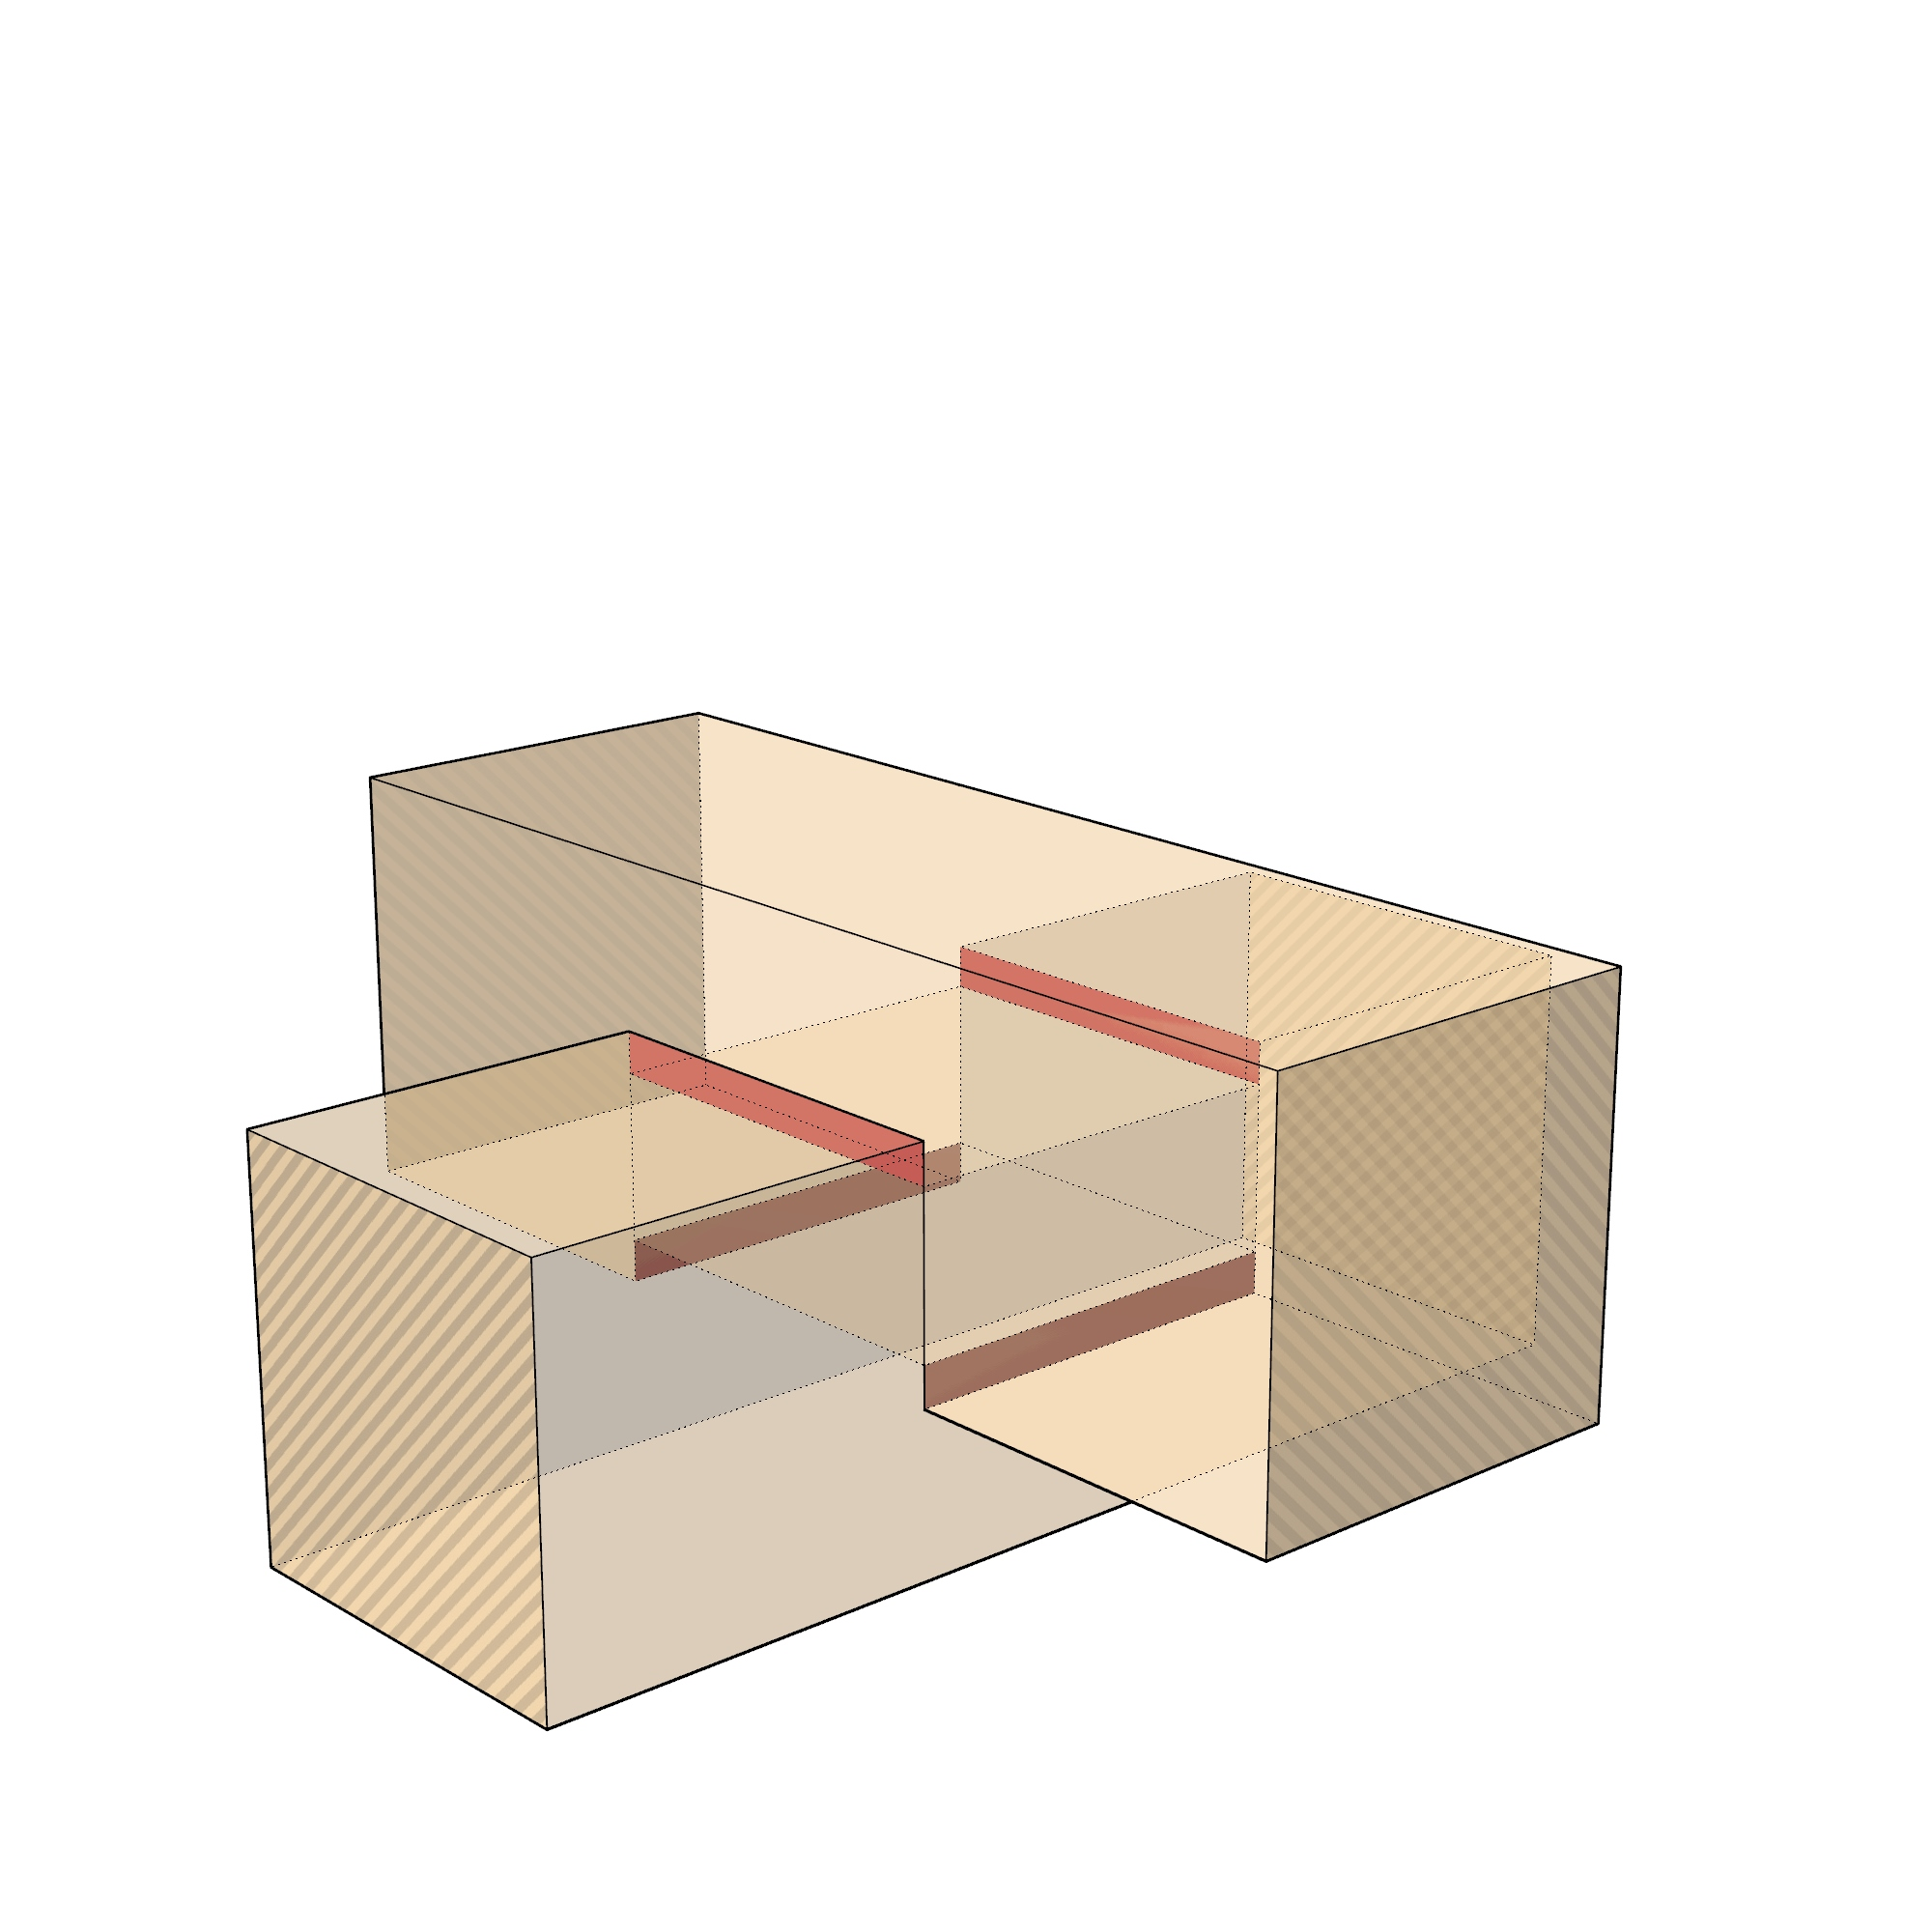
\includegraphics[width=\textwidth]{./images/image17.jpg}
\end{subfigure}
\hfill
\begin{subfigure}[b]{0.3\textwidth}
\centering
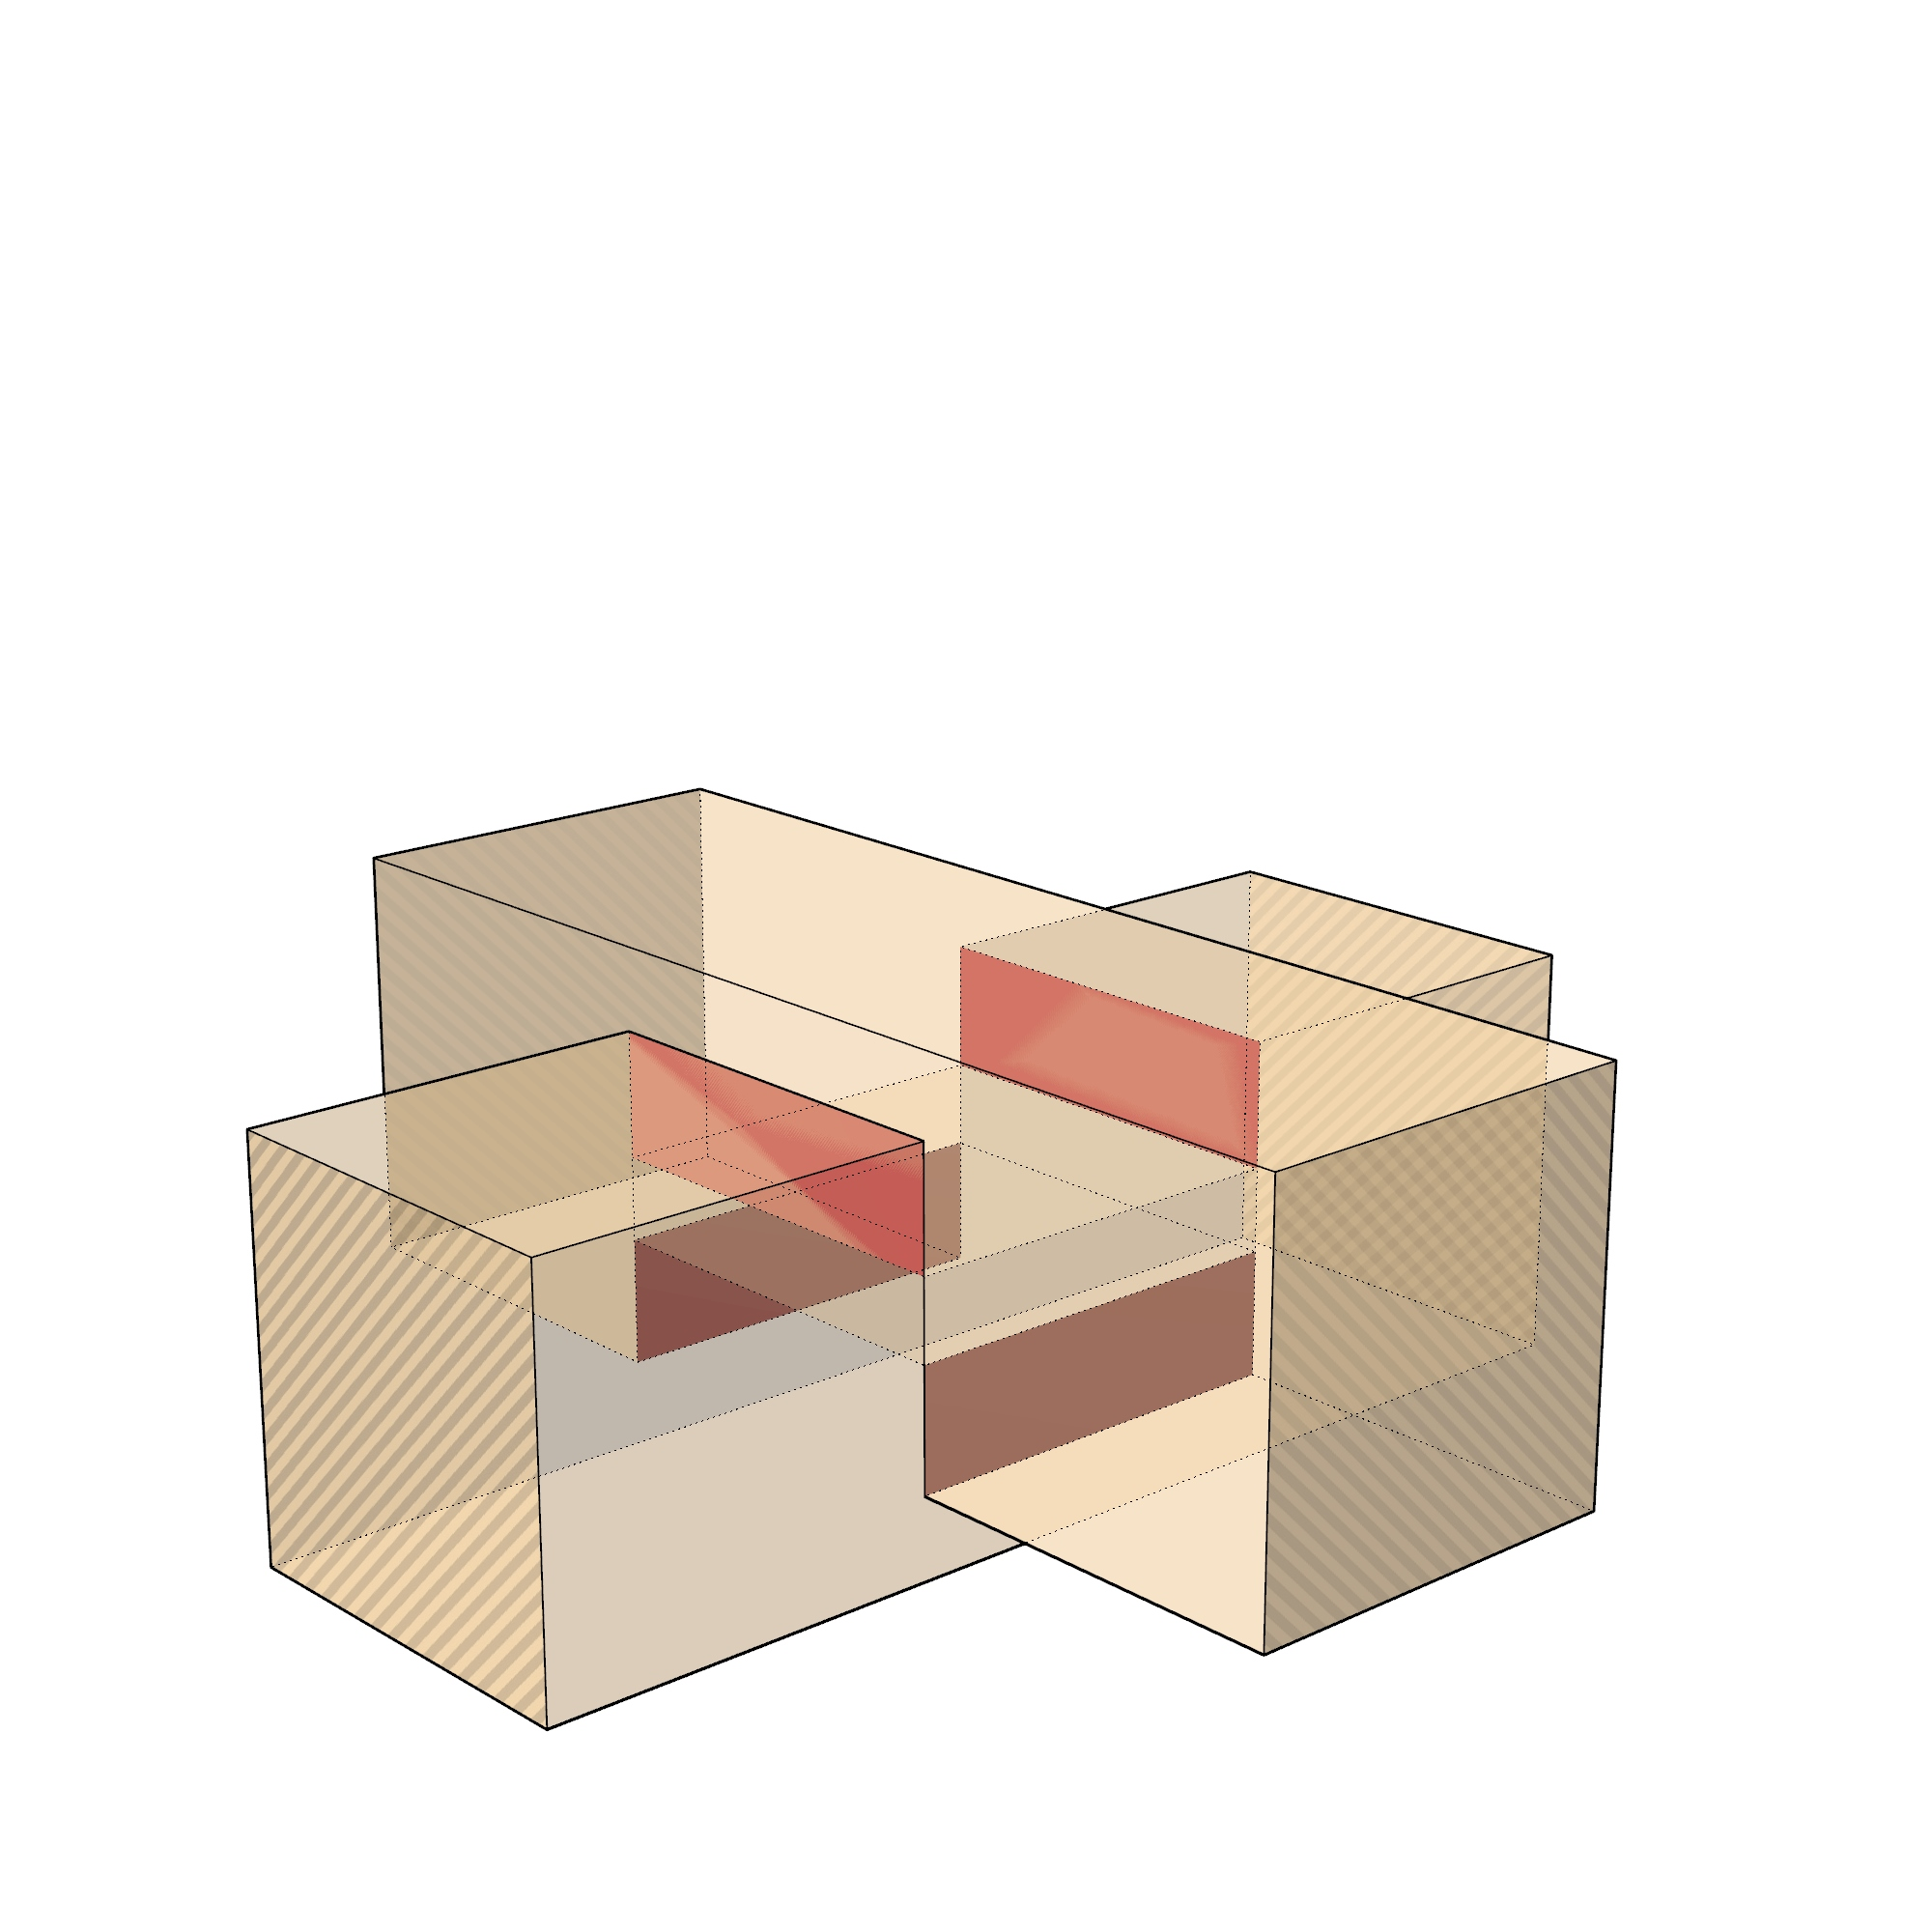
\includegraphics[width=\textwidth]{./images/image7.jpg}
\end{subfigure}
\hfill
\begin{subfigure}[b]{0.3\textwidth}
\centering
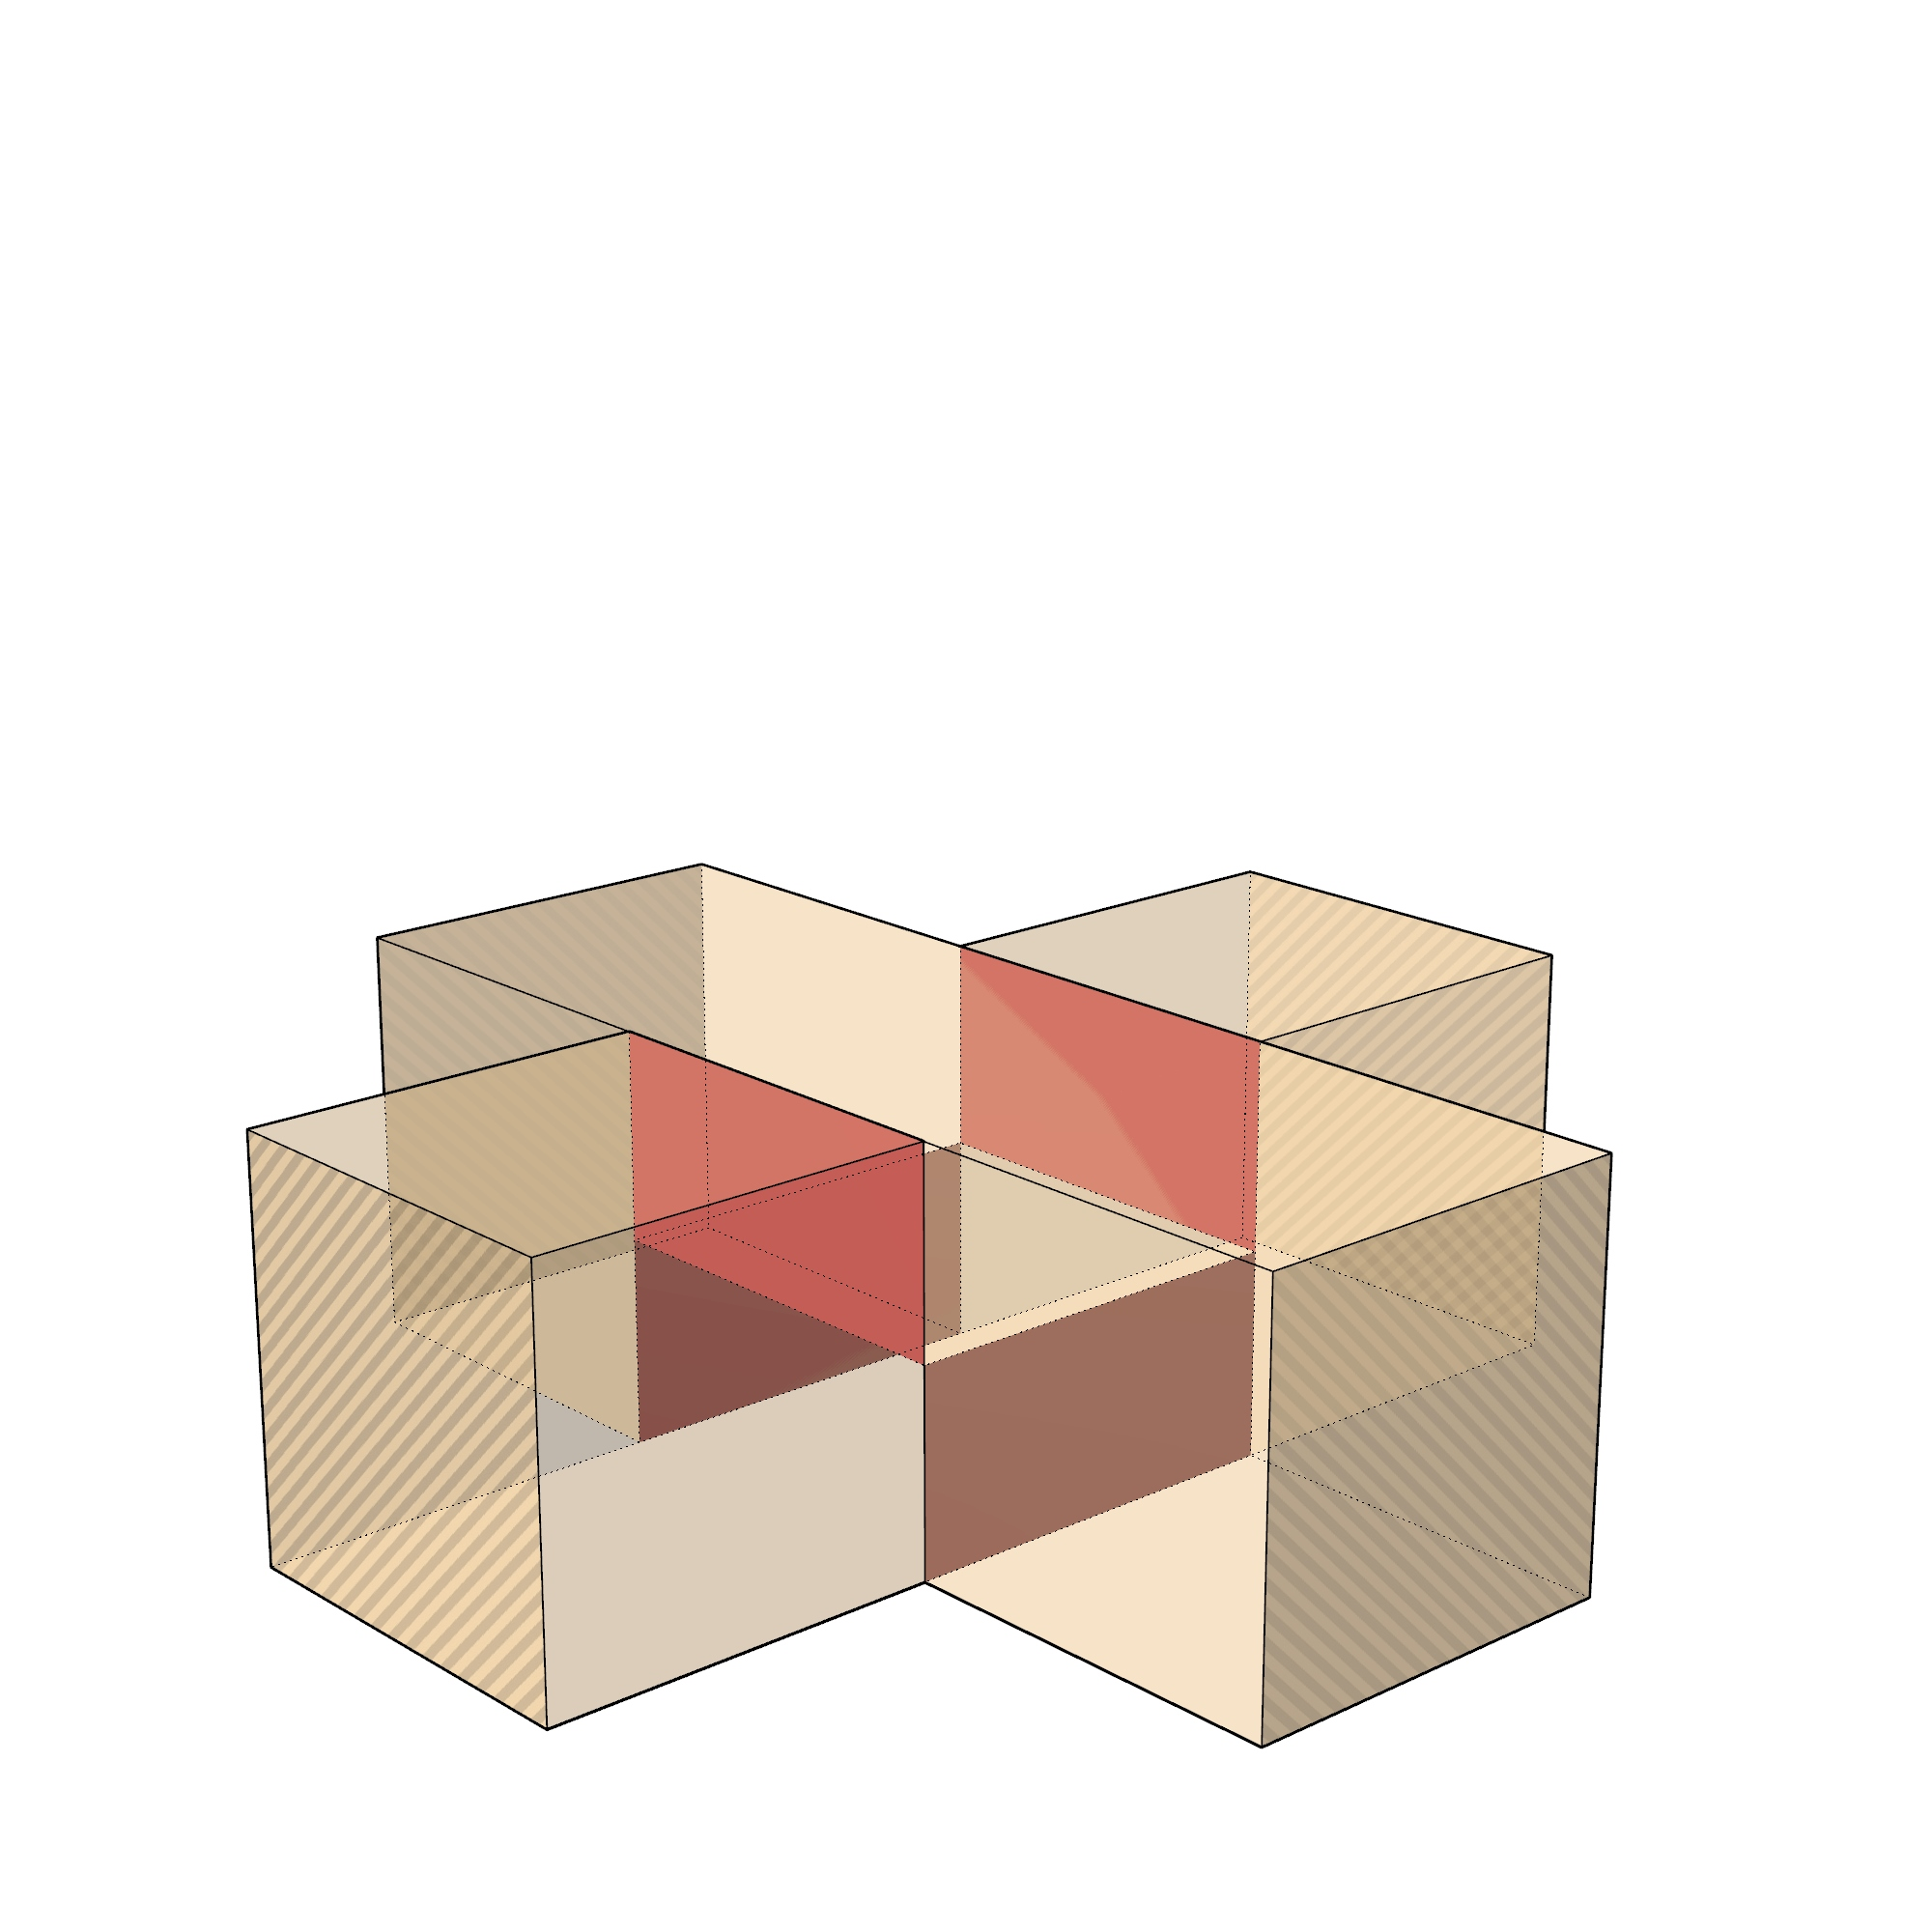
\includegraphics[width=\textwidth]{./images/image6.jpg}
\end{subfigure}
\end{figure}


\vspace{1\baselineskip}
The design of these contact surfaces are used for many different purposes. For example to introduce geometrical interlock \href{https://www.zotero.org/google-docs/?FoyCyy}{(Larsson et al., 2020; Song et al., 2012)}\textit{ }, improve load transfer \href{https://www.zotero.org/google-docs/?uGwPtv}{(Likos et al., 2012)}, improve structural stiffness\textit{ \href{https://www.zotero.org/google-docs/?vLOXsl}{}(Fang $\&$ Mueller, 2018)} or to improve stability against live load \href{https://www.zotero.org/google-docs/?PPcjqg}{(Jack Sobon, 2014)}. Depending on the geometry of the sliding surface (e.g. tapered vs parallel) and the quality of the machined surface (e.g. rough vs smooth surface) these rubbing surfaces introduce different amounts of sliding friction that must be overcome by force.

Carpenters have always been aware of the quality of the joints and how it affects the assembly difficulty. However, with the use of CNC controlled joinery machines, the fabrication tolerance can be controlled much more easily. It is worth mentioning that one precedent project has attempted to control the moisture of the wood to shrink it for reducing friction \href{https://www.zotero.org/google-docs/?Wr3WNi}{(Jenny et al., 2022)}. However the approach required heating the entire piece of wood, and would be difficult for larger scale structures.

\subsection{Tight Fitting Joints}

The second form of assembly-resistance is the fit of the mating joints. Fit is a measurement of the tightness of the connection between two mating parts. The fit can be categorised into three main types: clearance fit, transition fit, and interference fit. Clearance fit allows for some play between the parts, whereas interference fit requires force to assemble the parts and creates a tight, secure connection. Transition fit lies between these two extremes, providing a snug fit with some allowance for slight variations in the parts' dimensions.

Various factors can influence the fit of the mating joints, such as machining tolerances \href{https://www.zotero.org/google-docs/?FYX9pE}{(Thibaut et al., 2016)}, movement of the timber after machining due to release of stress, and environmental conditions such as temperature and humidity change \href{https://www.zotero.org/google-docs/?2HzXKN}{(Cochran, 2018)}. 

Tighter fits can result in higher frictional forces, which may require more force to overcome during assembly. It can also increase the difficulty for the robot to align the joints to begin assembly, which may increase the failure rate. Conversely, looser fits can lead to lower frictional forces but may compromise the structural integrity or performance of the assembled components \href{https://www.zotero.org/google-docs/?uzXtzz}{(Robeller et al., 2017)}.

Existing studies on the effects of timber joint fit are mostly focused on furniture scale joinery using hardwood and with glue \href{https://www.zotero.org/google-docs/?G6Rwhz}{(Elek et al., 2020; Koerner-Al-Rawi et al., 2020; Larsson et al., 2020; Likos et al., 2012)}. At the scale of timber frame construction, the choice of fit is typically based on the carpenter's experiences and historically proven norms \href{https://www.zotero.org/google-docs/?Gwwdvh}{(Chappell, 2011)}. Only one recent study reported on the force required for architectural scale timber joints for plate structures \href{https://www.zotero.org/google-docs/?saXZ5b}{(Robeller et al., 2017)}. 

In fact, much of the architectural scale robotic assembly research avoided the problem of tight fitting joinery at all due to the difficulty in assembling them, instead they use tangential connections \href{https://www.zotero.org/google-docs/?I1l6rV}{(Apolinarska et al., 2016; Gandia et al., 2018; Parascho, 2019)}, and butt joints \href{https://www.zotero.org/google-docs/?1HKFGK}{(Apolinarska et al., 2021; Thoma et al., 2018)} that did not require a large assembly force. However, these joint designs require an extra fastening step, such as glueing \href{https://www.zotero.org/google-docs/?uhxjvO}{(Gramazio Kohler Research, ETH Zurich, 2022; Helmreich et al., 2022)} and screwing \href{https://www.zotero.org/google-docs/?uAzdbA}{(Apolinarska et al., 2016, 2021; Thoma et al., 2018)} that is often performed manually. Even when integral timber joinery was involved, a loose fit was chosen to make the robotic assembly process easier. 

\subsection{Assembly Force vs Robots}

The need to apply a large assembly force to overcome sliding friction and tight fit is a challenging problem for robotic assembly. 

Industrial robots, with their long kinematic chains are good for agile motions and spatial manipulation but are not optimal for applying large assembly force, typical industrial robots have payload capacity under 300kg, which roughly translates to 3kN of force. This is no match even against a reasonably tight timber joint at architectural scale. Even for special robots (e.g. palletizing and foundry robots) where the payload carrying capacity is high, they are bulky and heavy and are difficult to be integrated with a larger gantry system for architectural scale operation. 

The second challenging reason is that the large assembly force has to be applied directly on the mating joints. Considering that the most reasonable way for a robotic arm to hold a piece of timber would be from the middle, near its centre of gravity, the holding position would unlikely be where the joints are. For example, if a beam has two mating joints on the two ends, the pushing forces from the robotic arm would have to transfer through the length of the beam, by bending it, before it reaches the joints. Considering the low stiffness of the material, even if the robotic arm is strong enough, the strong pushing force would result in substantial bending or even damaging the beam. 

The third challenging reason is that there are more than one mating joint to be closed when assembling a beam. It is well known that the assembly of all the joints must proceed synchronously, or else the beam would jam and get stuck \href{https://www.zotero.org/google-docs/?tb7dgL}{(Dupont $\&$ Yamajako, 1994)}. Therefore, even if a robot could push from the centre of the beam without damaging it, any slight imbalance in the joint resistance among mating joints would result in a large torque on the wrist of the robotic arm. If the robot used a stiff control, this would likely result in an overload. If the robot used a compliant control, the beam would start to rotate and quickly get stuck. 

The fourth challenging reason is that a strong pushing force requires an equally strong reaction force that can support the other side of the mating joint. Therefore, even if a super robotic arm would be possible and the timber beam is not jamming, it is impossible to guarantee that the supporting force can be transmitted from the ground through the partially assembled timber structure without damaging what has already been built. The only possible alternative is to engineer a special end-effector to provide both the pushing force and the support at the same time, similar to the configuration of a clamp or a parallel gripper.

The fifth challenging reason is that the location and amount of timber frame joints can vary substantially between different elements in a timber frame structure. In addition, the shape of the joints are also variable, depending on the intersecting angles between the beams. Therefore even if a clamping end-effector concept is used, it is difficult to design it to accommodate different joint locations and joint angles. A severe limitation in the design possibilities would likely defeat the purpose of using robots to assemble structures in the first place. Perhaps this end-effector method would be possible for special cases where the joints are always at a similar location. For example, certain space frames with a topologically repetitive arrangement \href{https://www.zotero.org/google-docs/?UUeya7}{(Apolinarska et al., 2021; Willmann, Knauss, et al., 2016)}. 

An alternative approach that was considered is to use more than one robotic arm, each holding a clamping end effector near the joints. However, it is challenging to scale up for more complex arrangements as the number of robots will have to increase with the number of simultaneously assembled joints. While this may be possible for a two-robot scenario, more robots will simply not fit in the limited space between them.

\subsection{Joint Alignment}

During the assembly of timber structures, it is necessary to accurately align the mating joints between the robot-sode and the stationary-side.

On the robot-side, the joints are located on the beam that is being held by the robot. Because these beams have to be assembled in non-repetitive targets, teaching cannot be used (see 1.3.1 Inaccuracy for non-repetitive targets). Therefore the end-effector that holds the beam is subjected to unmonitored deviation. If the timber elements are long, a small orientation error can cause a large positional deviation at the joints that are located far away from the robot wrist. Furthermore, long timber elements may also be slightly bent (permanent and static) or deflect (dynamic) due to its own weight, which further increases the deviation at the location where the joints mate.

On the stationary-side, the joints are spread across different elements in the partially constructed structure. Due to accumulated installation error, or deformation of the flexible timber structure, the location of the joints can deviate from where they are supposed to be. Moreover, the deviation among each of the joints may not be towards the same directions, making detection and correction difficult.

Because the robot targets are all extracted from a CAD model, unless there are active sensors monitoring the location of the joints on both sides, the joint pairs are likely to be subjected to misalignments which cannot be detected or corrected. Even if the misalignment can be detected, if there are more than one joint to align, correction may still be impossible due to conflicting deviation direction.

In the case where misalignment is severe and the problem is undetected, the subsequent robotic motion will not only fail but can also damage the timber parts. 

\subsection{Fastener Installation}

While many of the traditional timber frame joints contain no fasteners, some of them do, and for a multitude of reasons. For example, timber wedges are used to pull the joints tighter during assembly and can improve its stiffness; Timber dowels or pegs are used to prevent joint loosening due to live load; Metal dowels are used in contemporary designs to transmit shear force with metal plate connectors; Metal screws can be used to transmit tensile forces over a joint that would be hard to achieve using timber contact faces alone. 

The assembly of threaded fasteners is a common operation in the manufacturing industry \href{https://www.zotero.org/google-docs/?SLTLD9}{(Jia et al., 2019)}. Many different types of specialised end-effectors, robotic screwdrivers and screw feeding systems are designed to accommodate different types of screws. In timber construction, the automated assembly lines for prefabricated light-timber frame walls often have integrated screwdrivers and nail guns. Automated nailing has also been demonstrated for large-scale architectural construction \href{https://www.zotero.org/google-docs/?NCjCe0}{(Apolinarska, 2018; Apolinarska et al., 2016)}. However, most of these systems have been used for assembling planar assemblies and there are extra challenges when this has to be performed spatially. For example, handling long screws and non-orthogonal entry angles. Many of these precedence projects have resorted to assembling the screws manually \href{https://www.zotero.org/google-docs/?M7H4UY}{(Apolinarska et al., 2021; Thoma et al., 2018; Willmann, Knauss, et al., 2016)}. 

For timber frame construction with larger timber sizes, the screws used on the integral timber joints are often much larger than those used in the lighter timber systems. For other fasteners such as dowels and wedges, they are more specialised and have no automated precedence. 

\section{Computational and Design Challenges}

\subsection{Designing with Integral Timber Joints}

Timber frame structures often employ the use of integral timber joints that are interlocking, to restrict the movement of beams after assembly. In many cases, there is only one single direction in which the mating beams can be moved to assemble the joints. The arrangement of beams and the design of the interlocking joints works together to provide the stability and stiffness of a timber frame structure. However, this approach also creates a complex, interlocking system of parts that are difficult to design and analyse, not unlike the 3D interlocking puzzles commonly found in museum gift shops.

Carpenters have long understood that a successful timber structure is not only one that stands up, but also one that can be assembled. In the pre-digital era, the scale and complexity of large timber structures, such as pagodas, roofs, and bridges, required the most experienced master carpenters to design \href{https://www.zotero.org/google-docs/?FJwvT8}{(Hayman, 2021; Hewett, 2022; Müller $\&$ Widmann, 2022; Vandenabeele et al., 2018)}. Even today, one of the most challenging tasks when designing a complex timber structure is to ensure that the beams and their joints satisfy both structural and assembly requirements \href{https://www.zotero.org/google-docs/?cy6tn2}{(Chilton $\&$ Tang, 2016)}. 

\begin{itemize}
	\item Structural requirements include arranging beams into a stable and functional structural system and designing the joints to transmit structural forces. 

	\item Assembly requirements include ensuring that all components can be manoeuvred into place, accounting for the constraints imposed by the interlocking joints, and verifying that the assembly sequence does not create conflicts or blockages \href{https://www.zotero.org/google-docs/?81R5f7}{(Wang et al., 2021)}. 

\end{itemize}
Historically, successful timber frame designs were passed from one generation of carpenters to the next, each of them making iterative improvements. Particularly successful designs, such as post-and-beam structures and long-span roof trusses became a typology that was repeated and used many times \href{https://www.zotero.org/google-docs/?u1rNPf}{(Jack Sobon, 2014; Sobon $\&$ Schroeder, 1984)}.

Today, advances in the computer graphic field have created many analytical methods and opened up new possibilities for designing and analysing novel timber structures. In this thesis, structural analysis and assembly analysis will not be the core focus of the research. This is because they are already a highly established field and that many existing works have already studied them in depth. However, it is still necessary to be aware of their challenges to be able to apply the techniques correctly.

\subsection{Structural Analysis}

Timber structures are designed by considering various factors such as material properties, structural loads, environmental conditions, building codes, and aesthetics. The process typically begins with architectural design, where the overall form and layout of the building are determined. This is followed by structural design, where the appropriate sizes and shapes of timber members, connections, and joints are selected to ensure structural integrity, stability, and longevity.

Timber structures, particularly those with integral timber joints, present unique challenges in terms of analysis due to the complexity of the joint behaviour, material properties, and load distribution. These challenges can make it difficult to accurately predict the structural performance and ensure the safety and longevity of the structure. Some of the key challenges in analysing integral timber joints are:

\begin{itemize}
	\item \textbf{Anisotropic material properties} - The mechanical properties of wood material vary along different directions. This anisotropy can affect the behaviour of integral joints, as the strength and stiffness of the joint depend on the direction of the applied loads and the orientation of the wood fibres. Accurate analysis must account for these variations in material properties \href{https://www.zotero.org/google-docs/?L0yiAX}{(Thelandersson $\&$ Larsen, 2003)}.

	\item \textbf{Non-linear behaviour - }The behaviour of timber material and timber joints can be non-linear, particularly under high load levels or in the presence of defects, such as cracks or knots. This non-linear behaviour can complicate the analysis process, as it requires more advanced numerical methods and computational models to accurately predict joint performance \href{https://www.zotero.org/google-docs/?BE40wh}{(Gustafsson, 2003; Tanadini $\&$ Schwartz, 2021)}.

	\item \textbf{Moisture content and hygroscopicity -} Wood is hygroscopic, meaning it absorbs and releases moisture in response to changes in environmental conditions. This can cause dimensional changes and affect the mechanical properties of the timber, impacting the behaviour of integral joints. Accurate analysis must account for these moisture-related effects and their potential impact on joint performance \href{https://www.zotero.org/google-docs/?6q9alE}{(Thelandersson $\&$ Larsen, 2003)}.

	\item \textbf{Load distribution and interaction -} Integral timber joints often involve complex load distribution and interaction between multiple components. This can make it difficult to accurately predict the load-carrying capacity and failure modes of the joint. Advanced structural analysis techniques, such as finite element analysis (FEA), are often required to accurately model these interactions and predict joint behaviour .

	\item \textbf{Uncertainty in material properties and geometric tolerances -} Variability in material properties, such as strength and stiffness, as well as uncertainties in geometric tolerances, can make it challenging to predict the behaviour of integral timber joints with high confidence. Probabilistic approaches, such as reliability analysis \href{https://www.zotero.org/google-docs/?Xd18TY}{(Ranta-Maunus et al., 2001)} and stochastic finite element methods \href{https://www.zotero.org/google-docs/?mnlFCb}{(Kandler et al., 2015)}, can be used to quantify these uncertainties and assess the impact on joint performance.

\end{itemize}
\subsection{Assembly Analysis}

Assembly analysis of timber frame structures with integral timber joints is a crucial aspect to ensuring the structure can be assembled, this is known as joint mobility analysis, or assemblability analysis. The assembly analysis can be extended to include automatic sequence planning and motion planning \href{https://www.zotero.org/google-docs/?JFbpMZ}{(Wang et al., 2021)}. Assembly problems can be further categorised \href{https://www.zotero.org/google-docs/?Ioe45z}{(Wang et al., 2021)} by their properties: 

\begin{itemize}
	\item Number of hands - number of simultaneously moving parts needed for assembly 

	\item Monotonicity - whether the parts can be assembled in one simple motion, or whether intermediate movements are needed.

	\item Linearity - whether the assembly motions are linear, rotational, helical or other freeform motions. 

\end{itemize}
Most of the precedence robotic assembly projects in the architectural field, including the timber frame assembly problem in this thesis, belong to the simplest option of all (single hand, linear and monotonic movements). Even for projects that have used more than one robot during the process \href{https://www.zotero.org/google-docs/?4QpBeT}{(Parascho, 2019; Thoma et al., 2018)}, unless it involves multiple simultaneous movements in different trajectories, they are still considered one-hand problems.

\begin{flushleft}
Large amount of research has been devoted to the automatic sequence and motion planning. For example, in the context of mechanical assembly\textit{ \href{https://www.zotero.org/google-docs/?AdSBUO}{}(Bahubalendruni $\&$ Biswal, 2016; De Fazio $\&$ Whitney, 1987; Homem De Mello, 1989; Wilson, 1992)}, computer graphics\textit{ \href{https://www.zotero.org/google-docs/?drprl1}{}(Natarajan, 1988; Wang et al., 2018)} and also timber construction\textit{ \href{https://www.zotero.org/google-docs/?NZFd5k}{}(Tai, 2012)}. It is also possible to include additional heuristics in the search of an optimal assembly plan. For example, to maximise structural stability during construction \href{https://www.zotero.org/google-docs/?qq9t2G}{(Deuss et al., 2014; Garrett et al., 2020)}, avoid robotic collision \href{https://www.zotero.org/google-docs/?noNjLm}{(Huang et al., 2016; Yu et al., 2016)} or to minimise assembly time.
\end{flushleft}


When robots are used to perform an assembly task, the assembly analysis mentioned above also has to consider the actions of the robots and the tools, and their physical limitations. These limitations include

\begin{itemize}
	\item \begin{flushleft}
\textbf{Collision }- The robot and parts attached to the robot must not come into collision among itself or with stationary objects \textit{(see \underline{5.2.7.1 Collision Checking})}.
\end{flushleft}


\end{itemize}
\begin{itemize}
	\item \textbf{Reachability }- The robot must be able to reach all the targets that are needed to manipulate the objects for their assembly \textit{(see \underline{5.2.7.2 Inverse Kinematics})}.

	\item \textbf{Payload and Accuracy - }Certain operations may not be possible due to the mechanical limitations of the robot.

\end{itemize}
The extension of these analysis into the design process includes:

\begin{itemize}
	\item \textbf{Automatic Sequence Planning - }Identical to the sequence planning above, concerned with the sequence among parts.

	\item \textbf{Automatic Task Planning}\ \ - Planning the discrete actions of the robot to assemble each part (e.g. open gripper, move, close gripper, etc.) \href{https://www.zotero.org/google-docs/?YRv70u}{(Homem De Mello, 1989)}

	\item \textbf{Automatic Motion Planning} - Finding the trajectory for the robot joint to follow, such that the attached end-effector moves from one target to another.  \href{https://www.zotero.org/google-docs/?dDVZq8}{(LaValle, 2006)}

\end{itemize}
\begin{flushleft}
In this thesis, task planning and motion planning are unavoidable for generating the robot programmes. However, sequence planning will not be studied. It is assumed that an experienced timber engineer, designer or carpenter can be tasked to determine the assembly order based on experience and intuition.
\end{flushleft}


\subsection{Task and Motion planning}

The use of robots for assembling timber structures requires careful planning and simulation to ensure that there are no unintended collisions. 

The basic task of picking up a beam carrying it to the assembly location may sound simple for a human worker. However, the planning work required for a robot to do the same is not only computationally hard, but also complicated to set up correctly. The parameters that have to be planned are:

\begin{itemize}
	\item \textbf{Tasks} - What are the sequence of operations for moving the robot joints and actuating the attached tools (e.g. opening and closing grippers)?

	\item \textbf{Grasp }- What pose (position and orientation) does the robot use to hold the beam? Does the robot need to change its grasp during the process?

	\item \textbf{Targets }- Where are the targets for the robot to reach at the start and end of a motion to pick or place a workpiece at the correct location.

	\item \textbf{Trajectories }- What is the continuous path (a series of static joint angles) that allows the robot and its attached objects to move from one target to the next?

\end{itemize}
The main challenge for spatial assembly is that there are many possible directions and orientation for assembling an element. This is in steep contrast to a layer-by-layer construction approach, where new elements can be assembled from the top \href{https://www.zotero.org/google-docs/?vZK1dq}{(Apolinarska et al., 2016; Gramazio Kohler Research, ETH Zurich, 2009)}. 

Many spatial assembly projects have used a rule-based strategy to programme the transfer path. For example, a common approach for beam transfer is to raise the beam to a safe height before traversing horizontally \href{https://www.zotero.org/google-docs/?SFqNJ2}{(Hack et al., 2020; Søndergaard et al., 2016)}. However, this approach is still limited by the obstacles at the final approach when the robot is near the partially-assembled structure. For structures that are assembled from the core towards the periphery, a strategy of approaching the target from the ‘outside’ can be used \href{https://www.zotero.org/google-docs/?aftLlm}{(Adel et al., 2018)}. 

A more generic strategy is to use a sampling-based motion planner as it has the ability to automatically search for a viable path while avoiding collisions. \href{https://www.zotero.org/google-docs/?wxRkWx}{(Gandia et al., 2018; Thoma et al., 2018)} This is critical if some of the beams have to reach into the small openings of a structure. However, one of the often cited knowledge gap remains at the automatic generation of robotic trajectories for large amounts of uniquely shaped and positioned elements \href{https://www.zotero.org/google-docs/?COr7LA}{(Eversmann et al., 2017; Gandia et al., 2018)}. Latest research developments have already created the interface to access planning tools from the robotics research field for planning architectural assemblies \href{https://www.zotero.org/google-docs/?LW23oL}{(Gandia et al., 2018; Parascho, 2019; Parascho et al., 2018)}. The most comprehensive method to date being a unified sequence and motion planning or a unified task and 

\subsection{Joint Modeling and Solving}

Joint Modeling and Solving refers to the computational process of creating and adjusting parametric models of integral timber joints, ensuring their compatibility and adaptability within the larger context of the timber frame assembly, while taking into account fabrication constraints, user customizations, and structural considerations.

Timber joints are typically modelled as a subtraction from the beam’s geometry. In many joint designs, both halves of the joints are not geometrically similar, therefore the subtraction geometries for the beams on each sides are also different. In order to ensure correct fit, it is necessary to ensure that both sides of the joint will match with each other. While this is relatively straightforward to achieve for one joint instance, a parametric joint model will need to adapt itself to different jointing angles between the beams. Because of the continuous nature of the joining angles, the model requires defining parametric geometrical relationships in 3D to create the solid models \href{https://www.zotero.org/google-docs/?Ix4BkB}{(Vestartas, 2021)}. In general, a parametric joint model will contain fixed properties that are dependent on the neighbouring beams, and editable properties that can be customised:

\textbf{Adaptation to the intersecting beams' position, size and angle -} This adaptability allows the joint geometry to be computed automatically by the intersecting beams without explicit modelling. Thus, changing the intersecting beams’ locations can trigger an update to snap it to a new position. The images below shows a mortise and tenon joint adapting to different beam intersection angles.

\begin{figure}[H]
\centering
\begin{subfigure}[b]{0.18\textwidth}
\centering
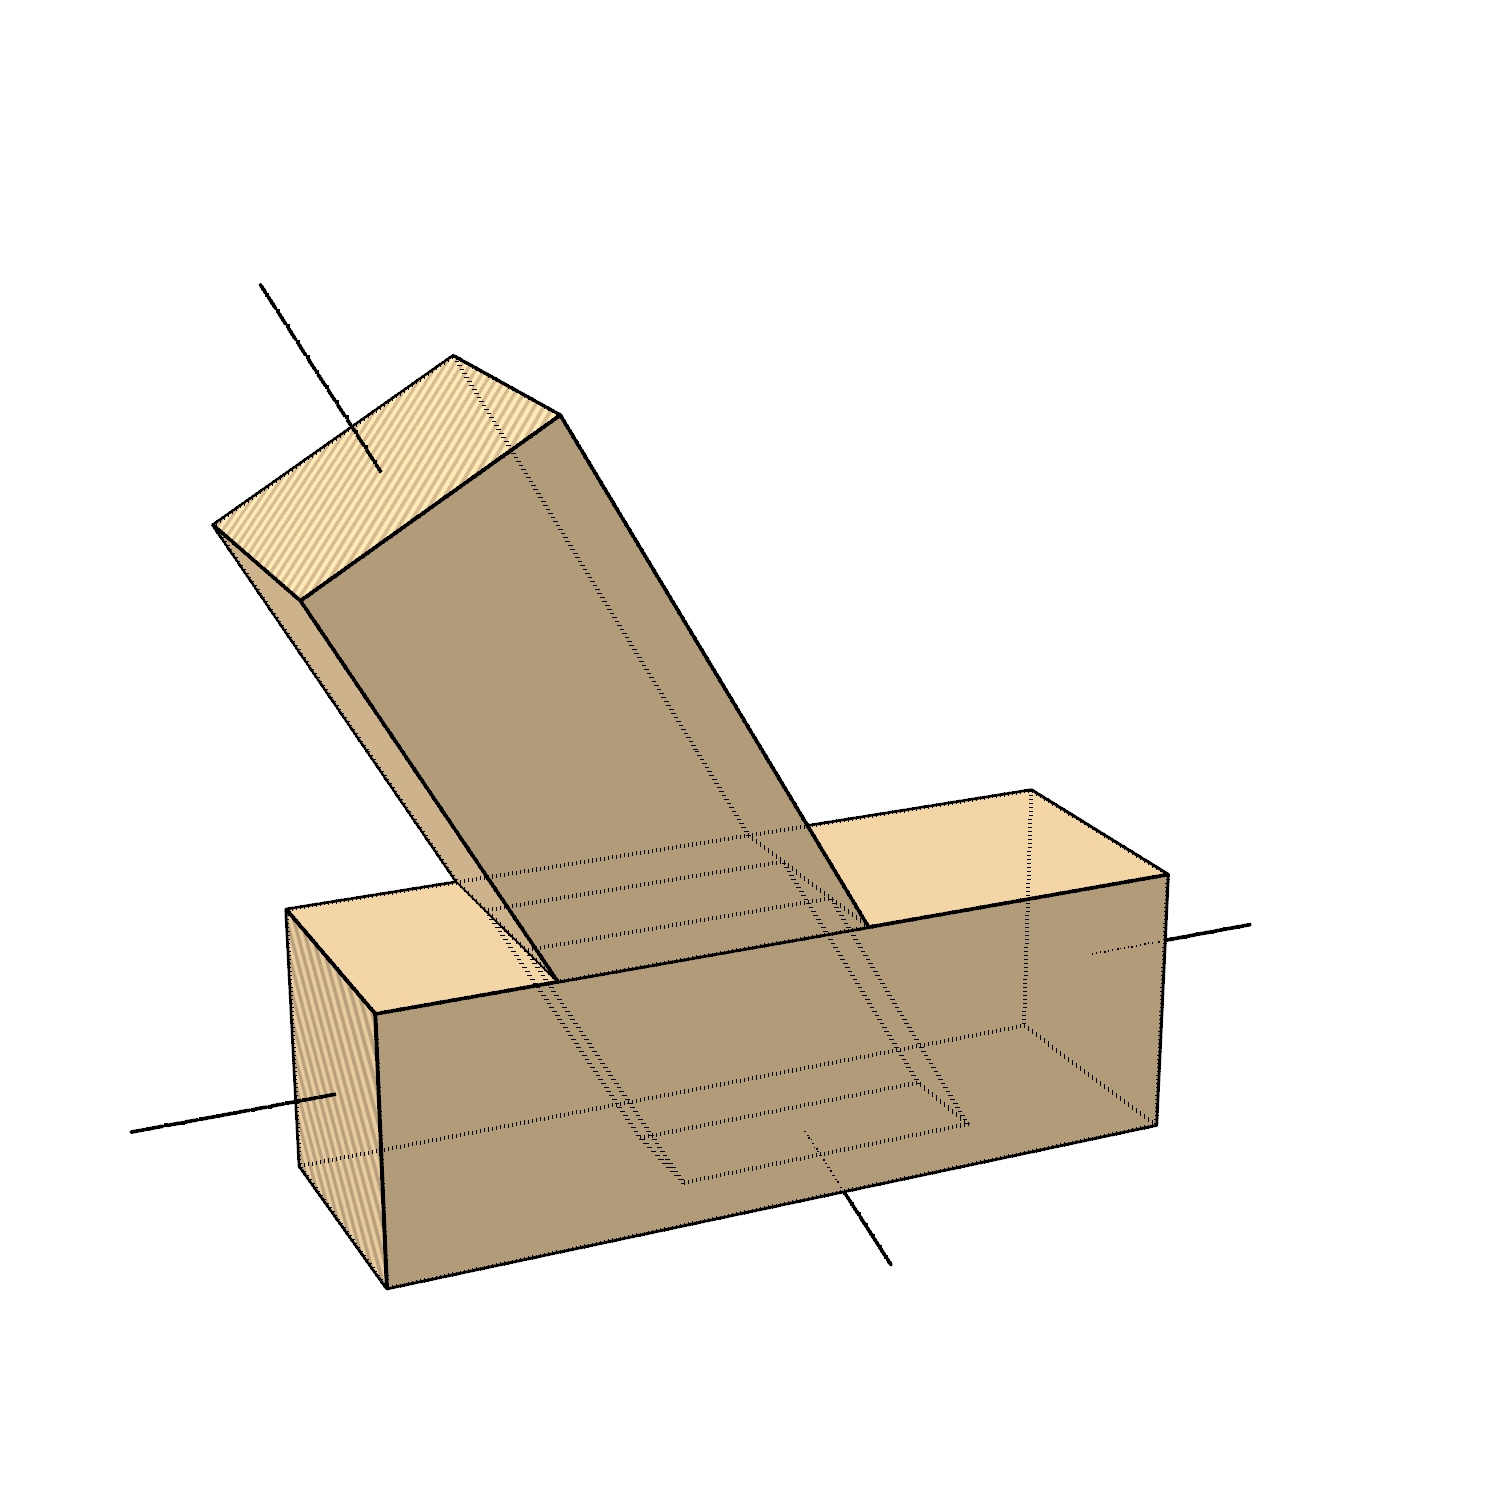
\includegraphics[width=\textwidth]{./images/image3.jpg}
\end{subfigure}
\hfill
\begin{subfigure}[b]{0.18\textwidth}
\centering
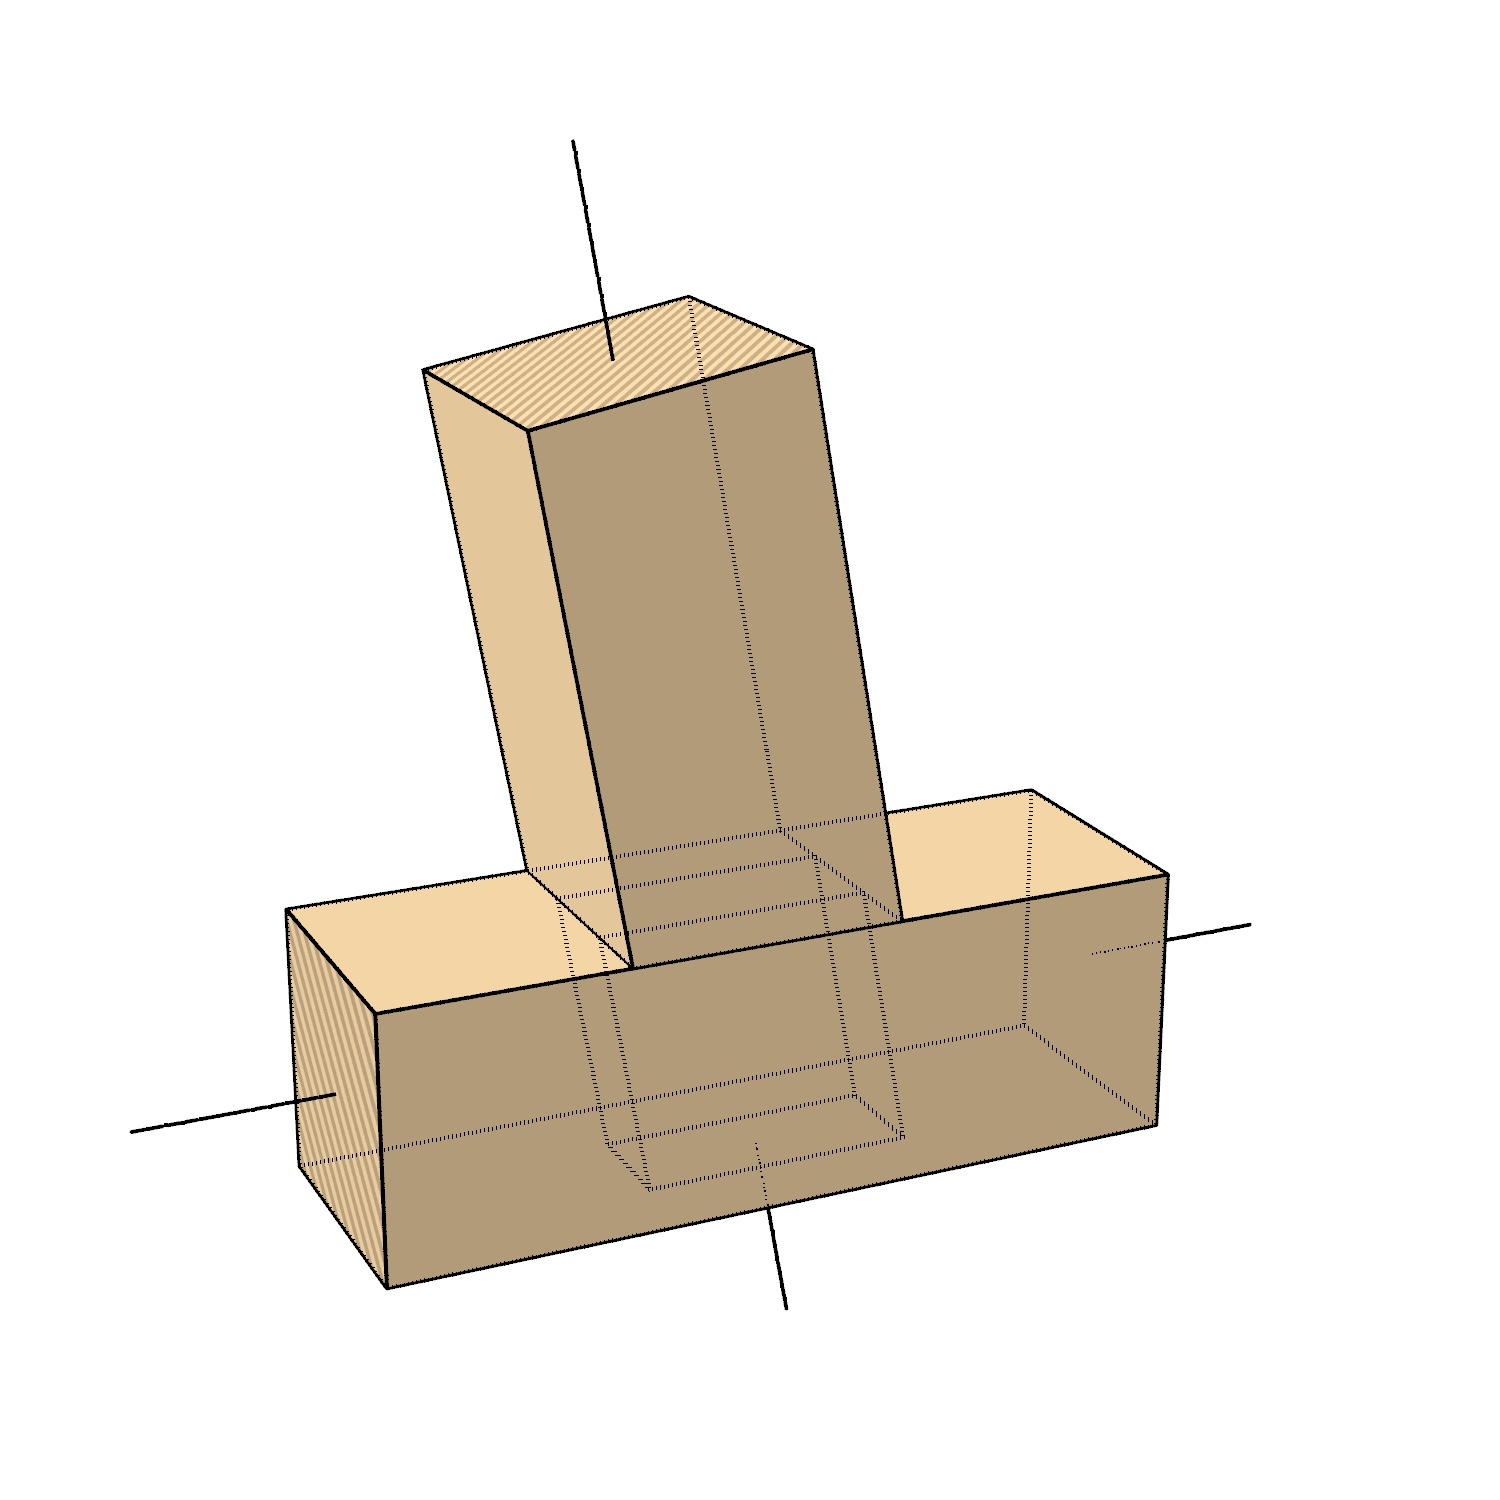
\includegraphics[width=\textwidth]{./images/image16.jpg}
\end{subfigure}
\hfill
\begin{subfigure}[b]{0.18\textwidth}
\centering
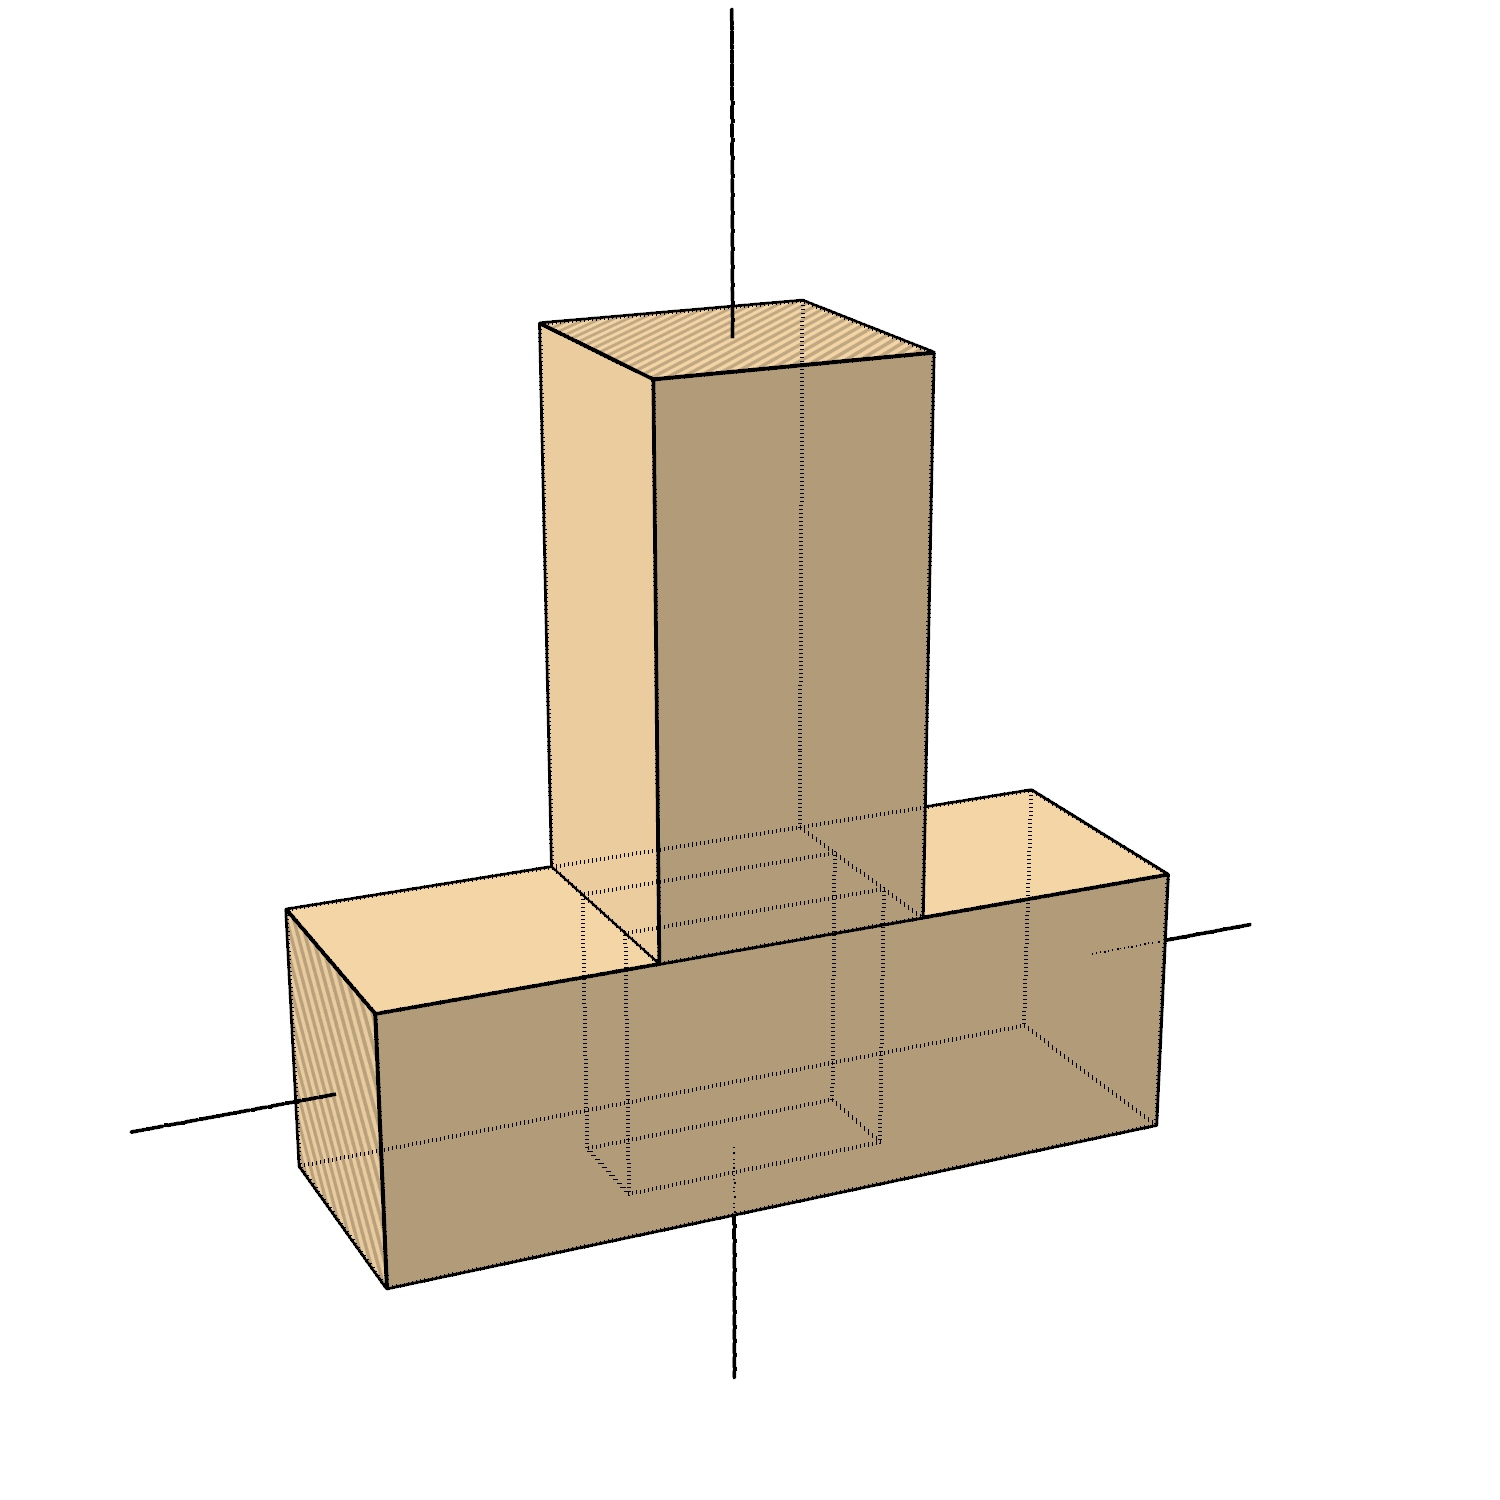
\includegraphics[width=\textwidth]{./images/image14.jpg}
\end{subfigure}
\hfill
\begin{subfigure}[b]{0.18\textwidth}
\centering
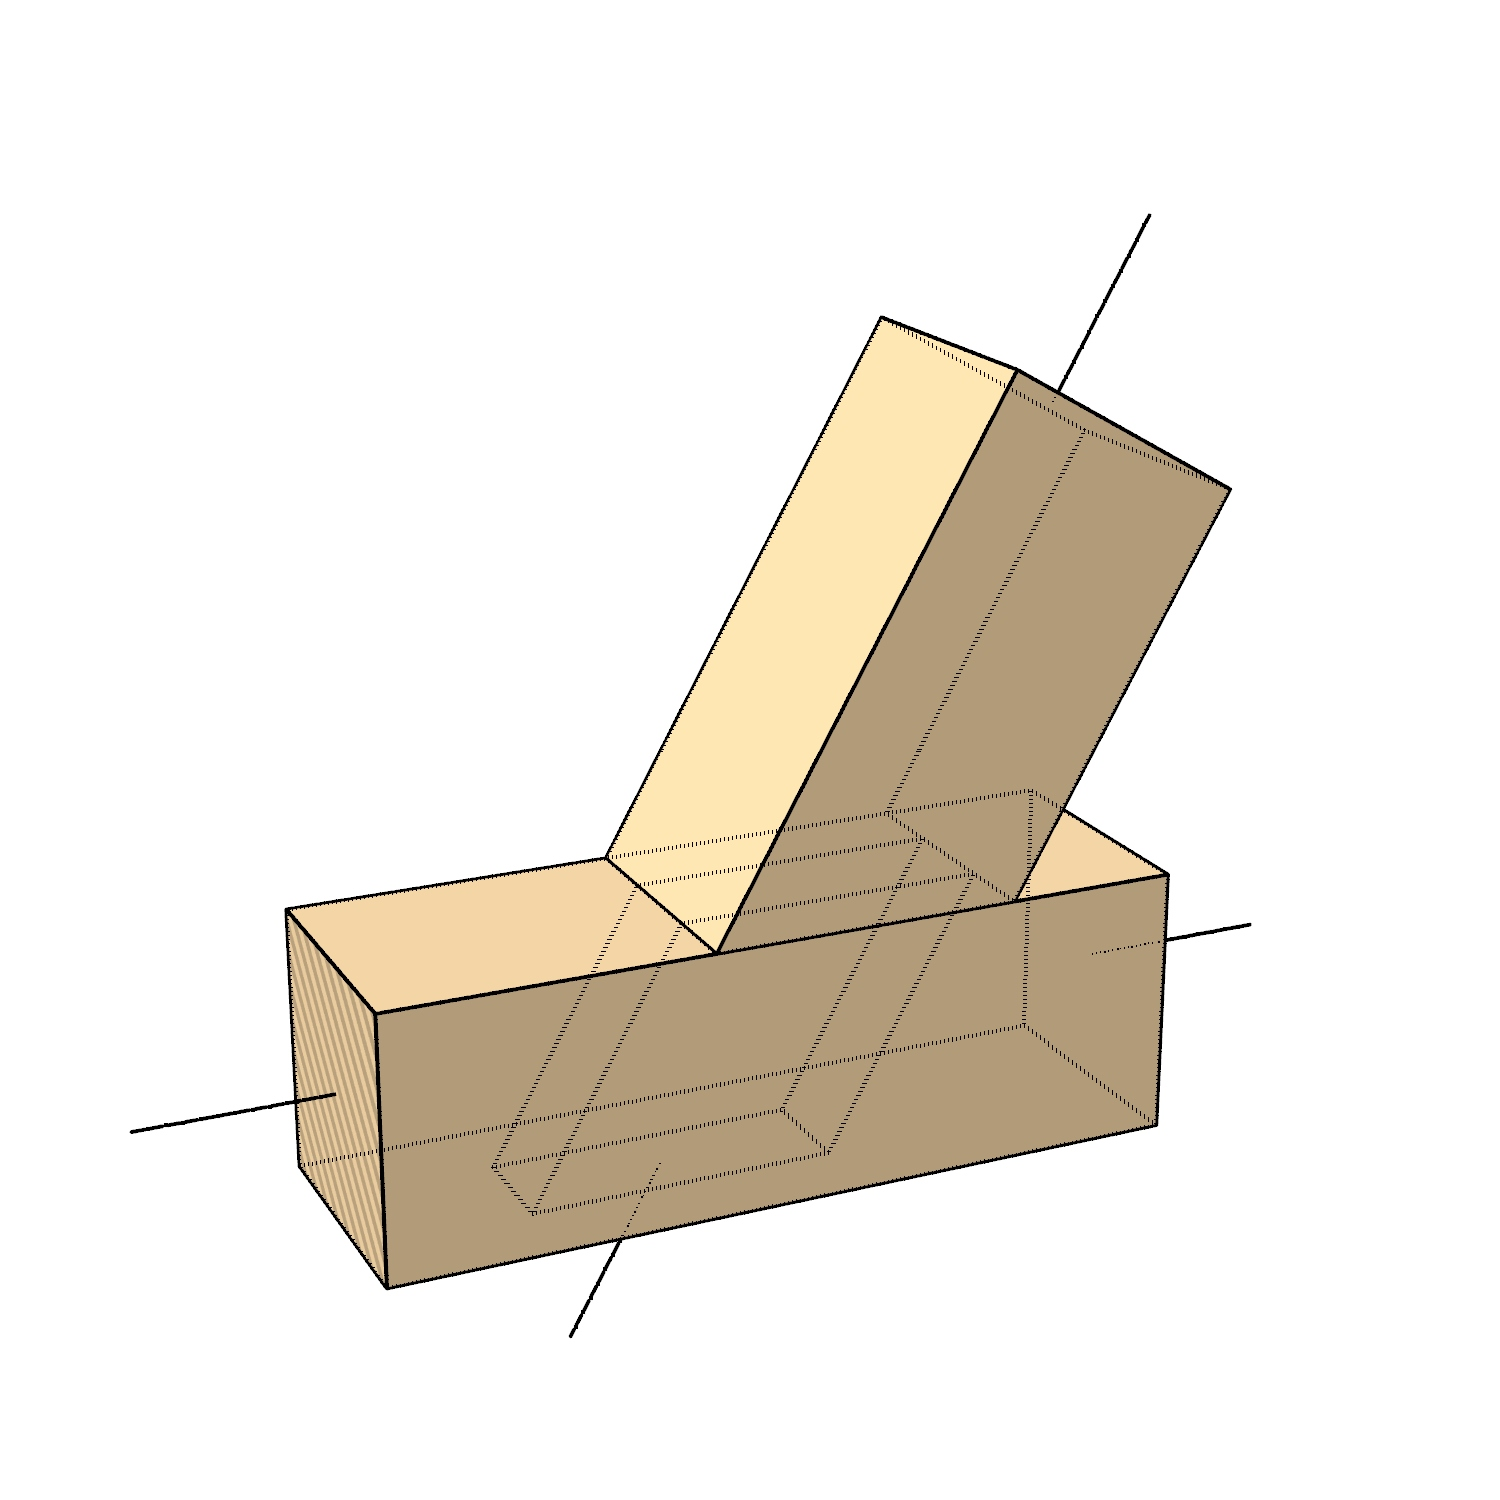
\includegraphics[width=\textwidth]{./images/image1.jpg}
\end{subfigure}
\hfill
\begin{subfigure}[b]{0.18\textwidth}
\centering
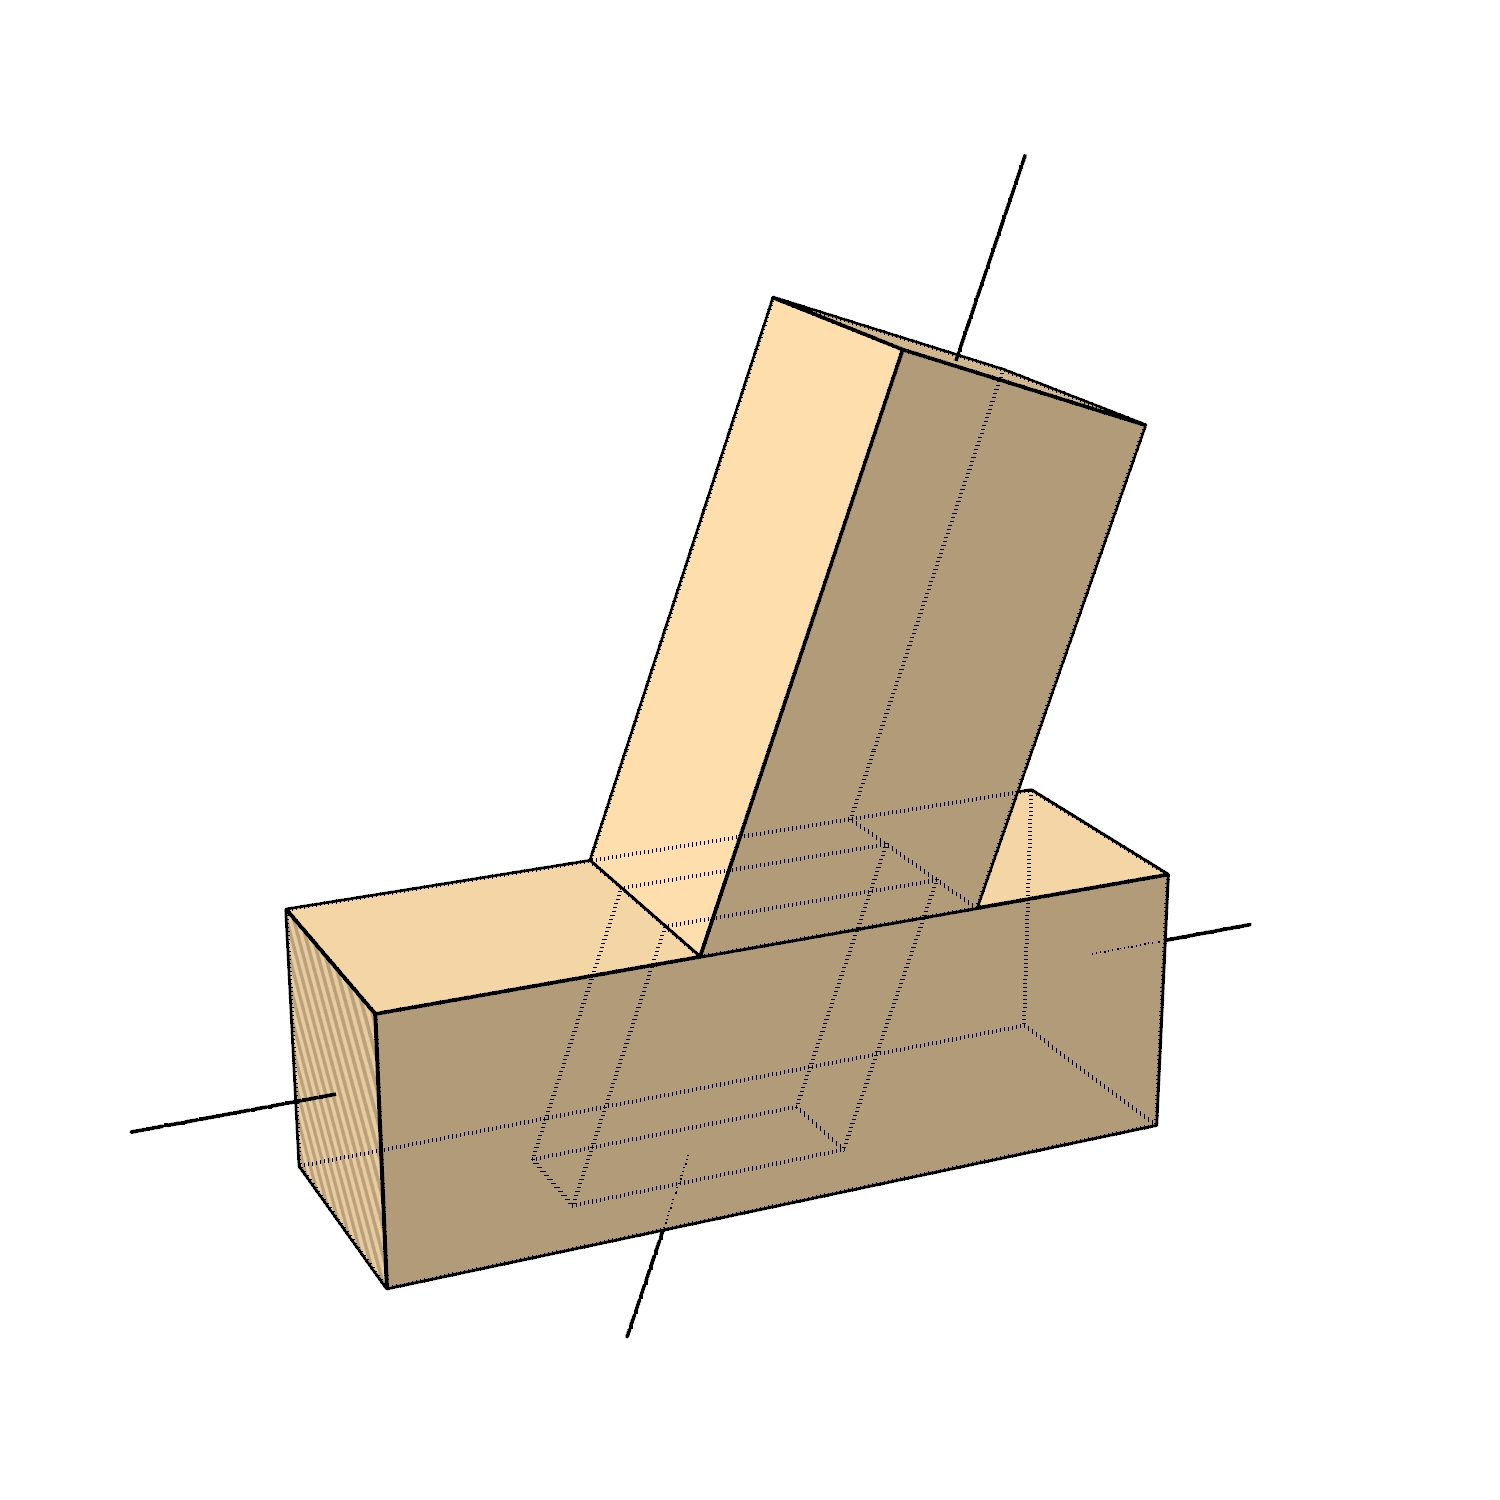
\includegraphics[width=\textwidth]{./images/image11.jpg}
\end{subfigure}
\end{figure}


\textbf{Customization of detail sizes or proportions - }Even a simple lap joint model can include an adjustable parameter for the cheek depth. More complex joint topology can have many adjustable parameters. \textit{(refer to the diagram of a housed dovetail T Lap having many parameters) }These adjustments are often useful for changing the structural behaviour of the joint and may be specified or changed at a later stage of the design process during engineering calculations. The images below show a mortise and tenon joint having the same intersection angles but different topologies. The proportion of the details in each topology would require a parametric definition.

\begin{figure}[H]
\centering
\begin{subfigure}[b]{0.18\textwidth}
\centering
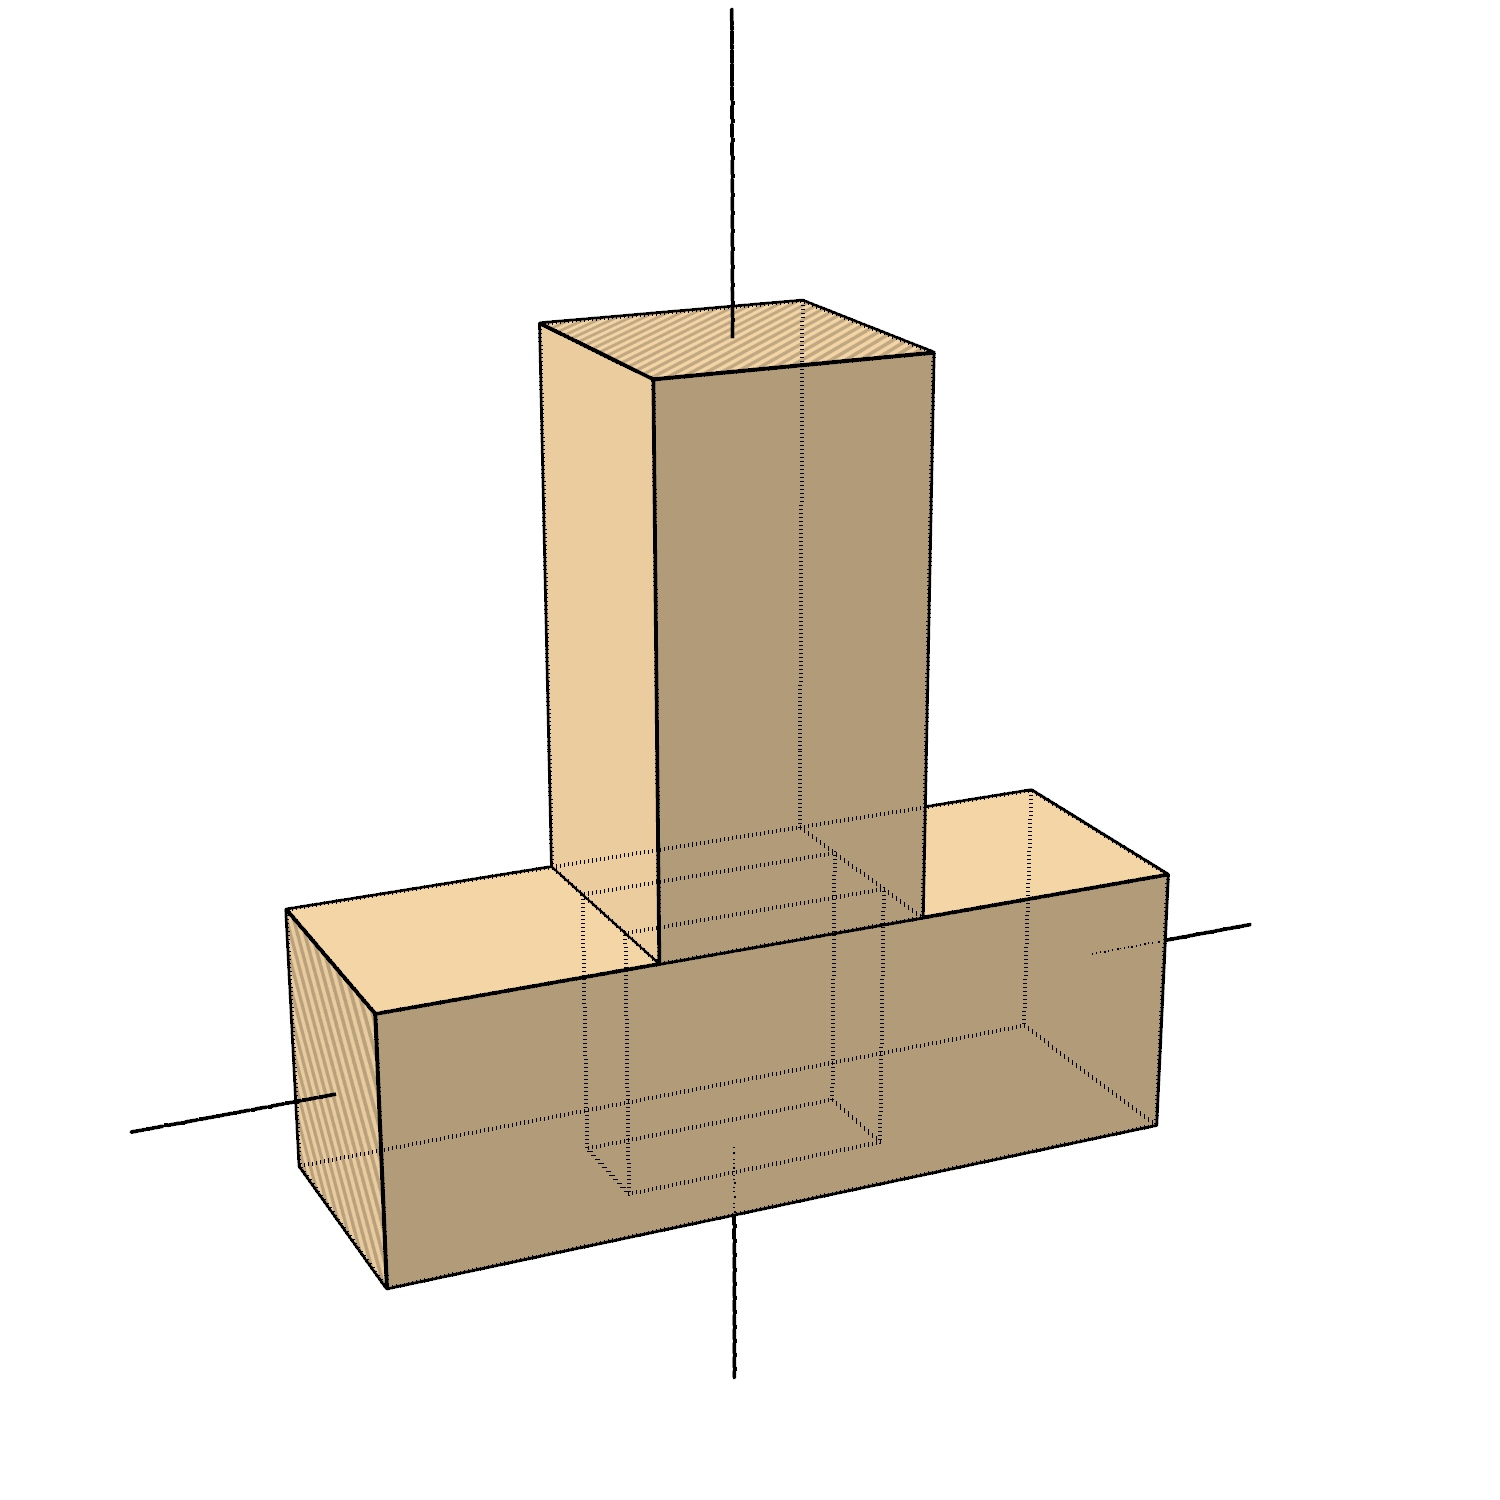
\includegraphics[width=\textwidth]{./images/image14.jpg}
\end{subfigure}
\hfill
\begin{subfigure}[b]{0.18\textwidth}
\centering
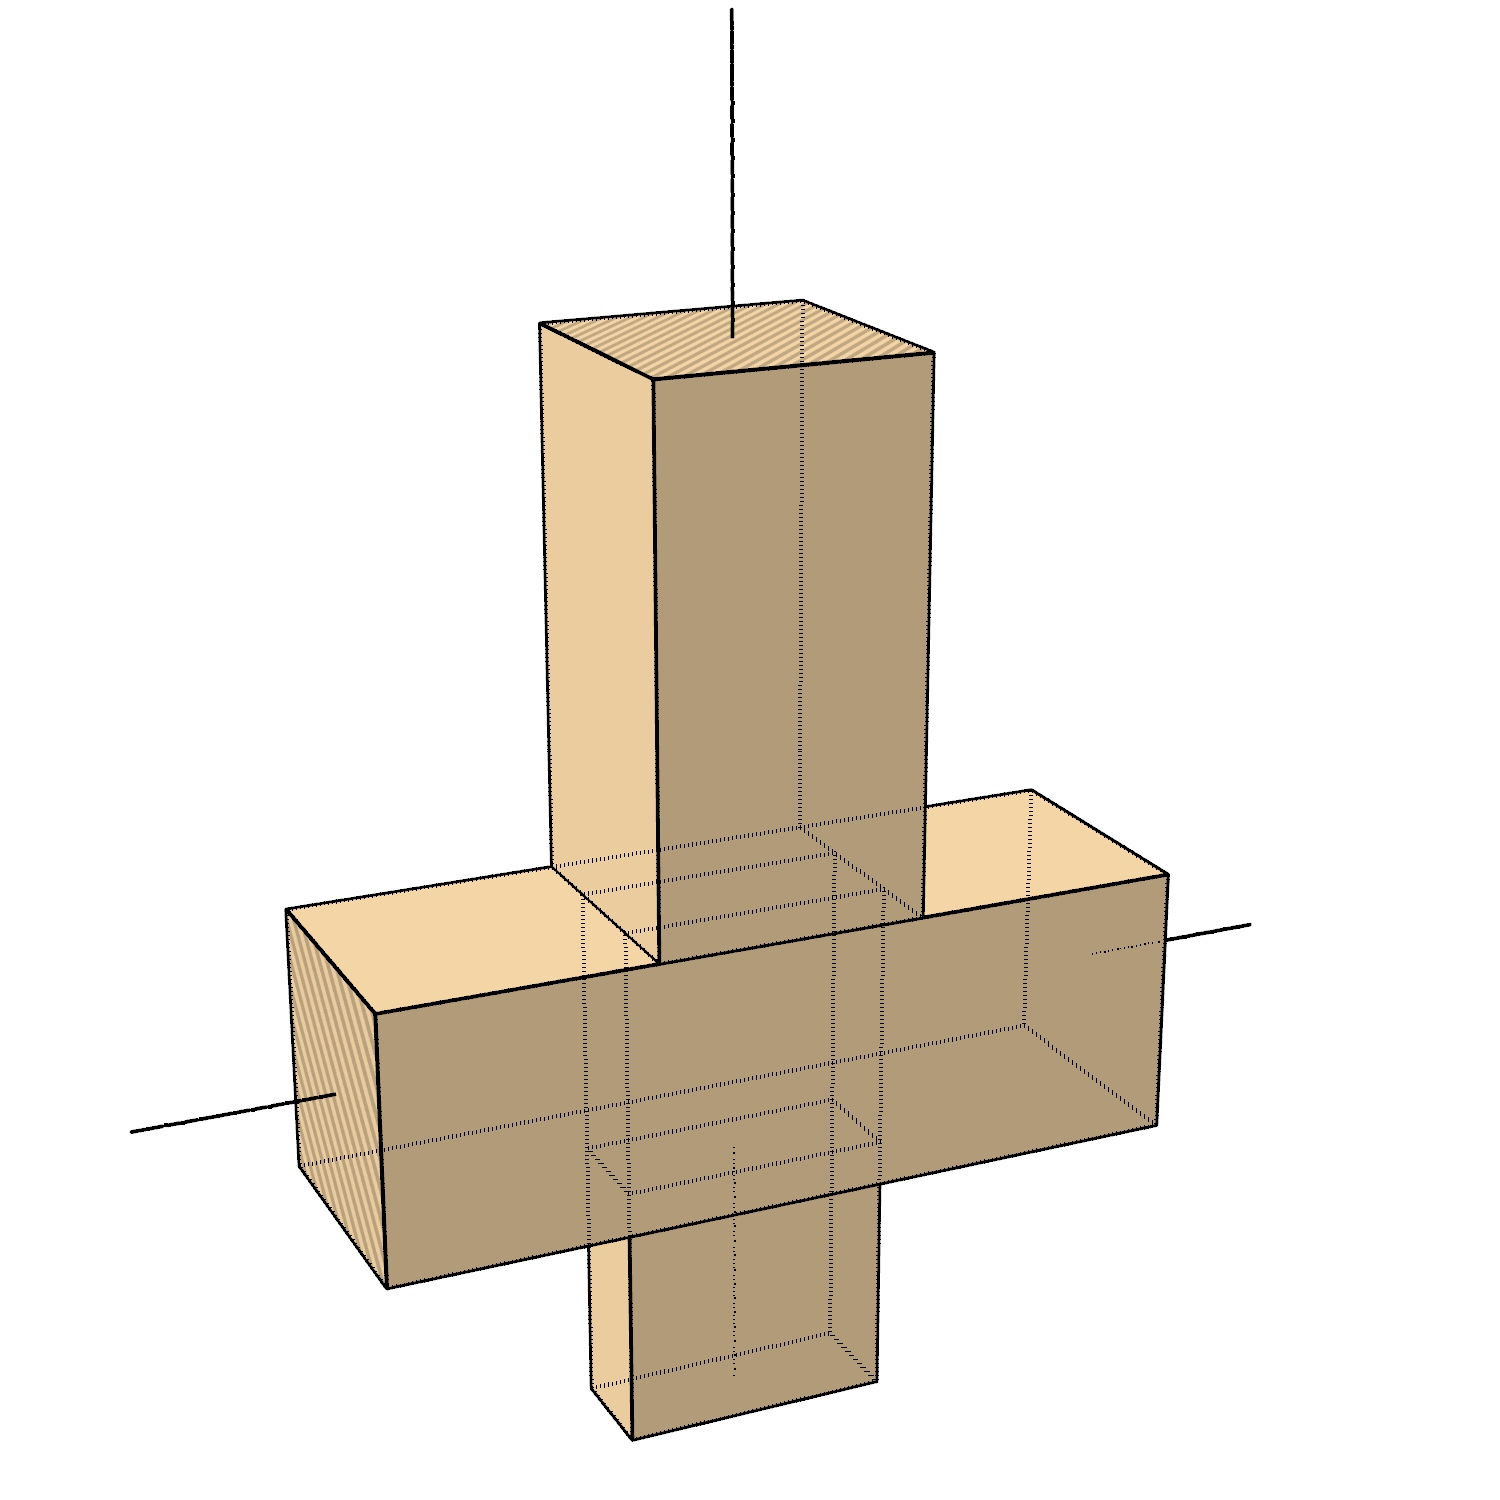
\includegraphics[width=\textwidth]{./images/image19.jpg}
\end{subfigure}
\hfill
\begin{subfigure}[b]{0.18\textwidth}
\centering
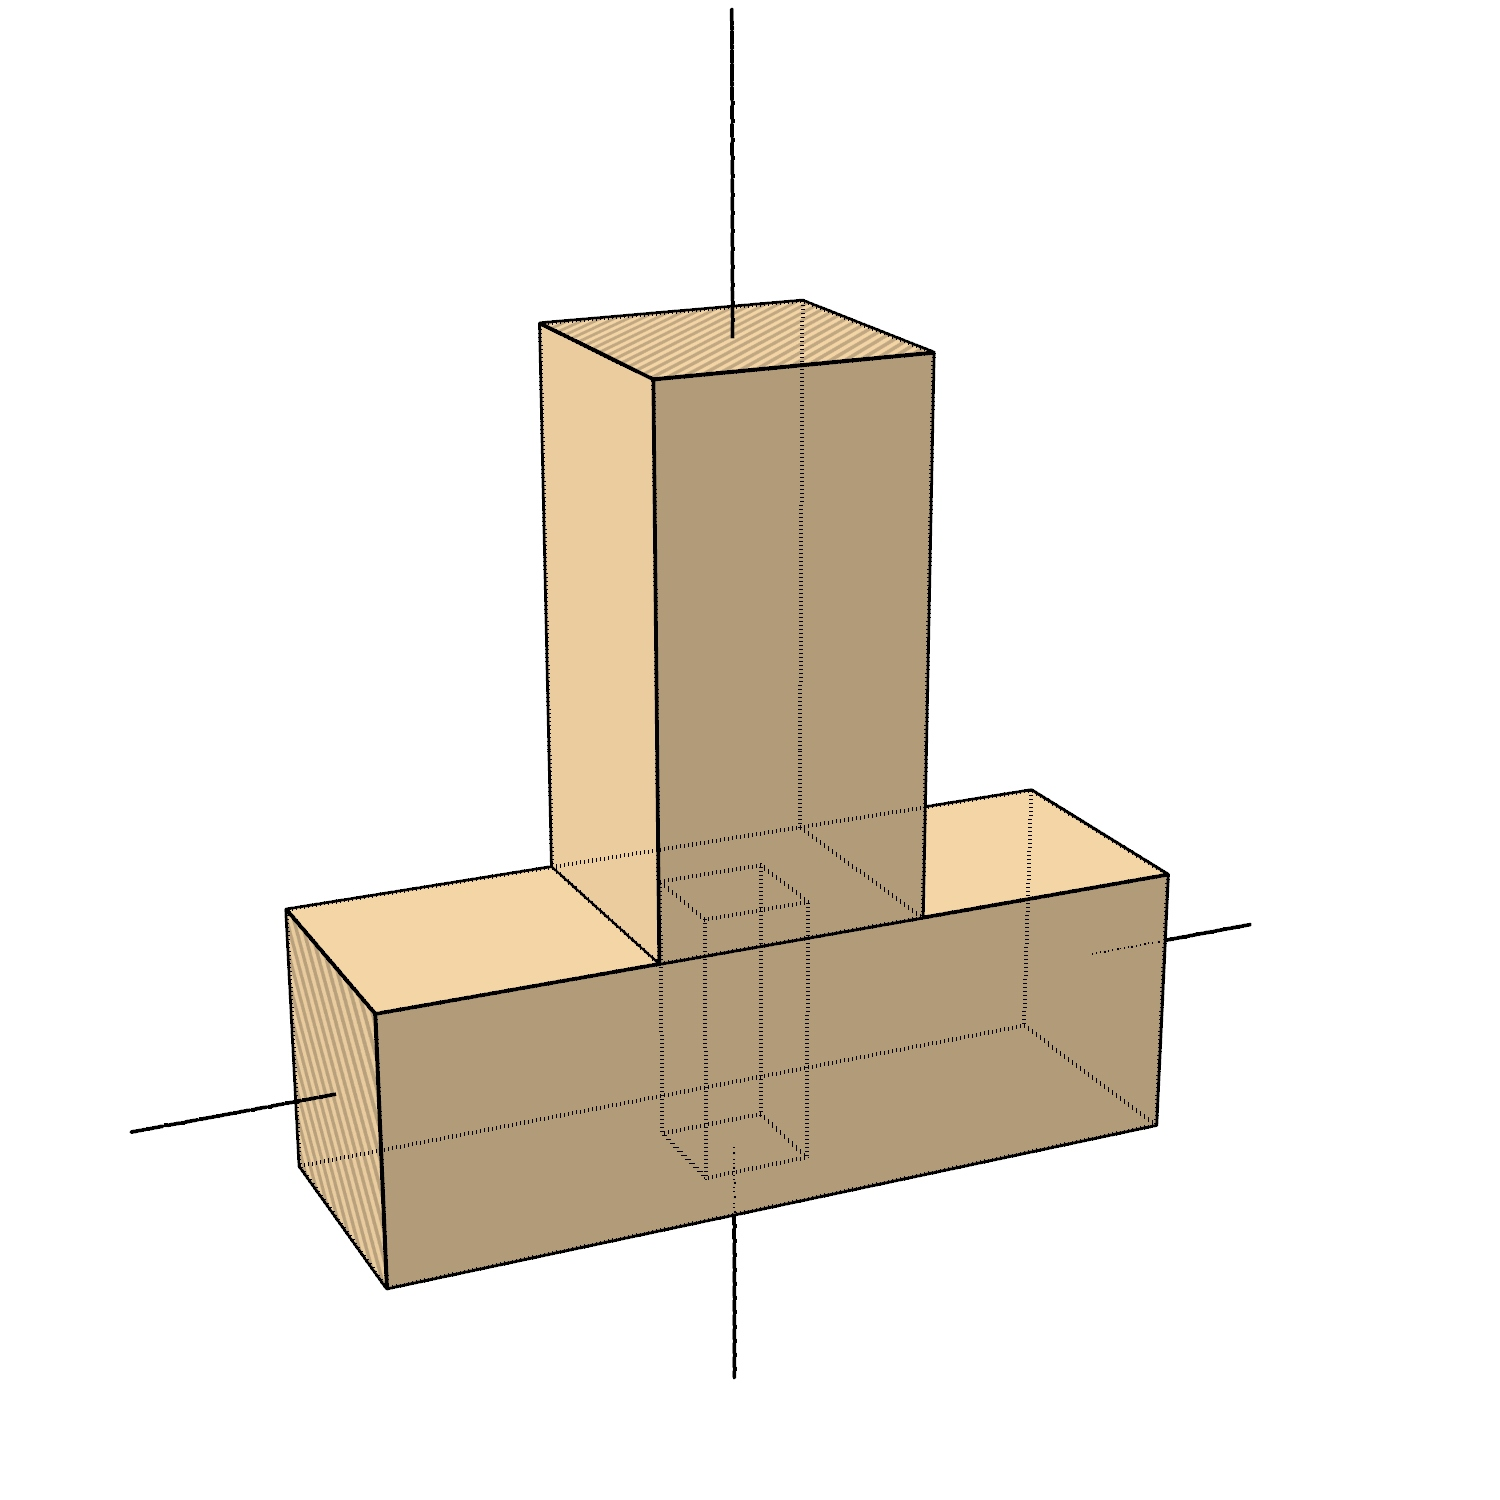
\includegraphics[width=\textwidth]{./images/image13.jpg}
\end{subfigure}
\hfill
\begin{subfigure}[b]{0.18\textwidth}
\centering
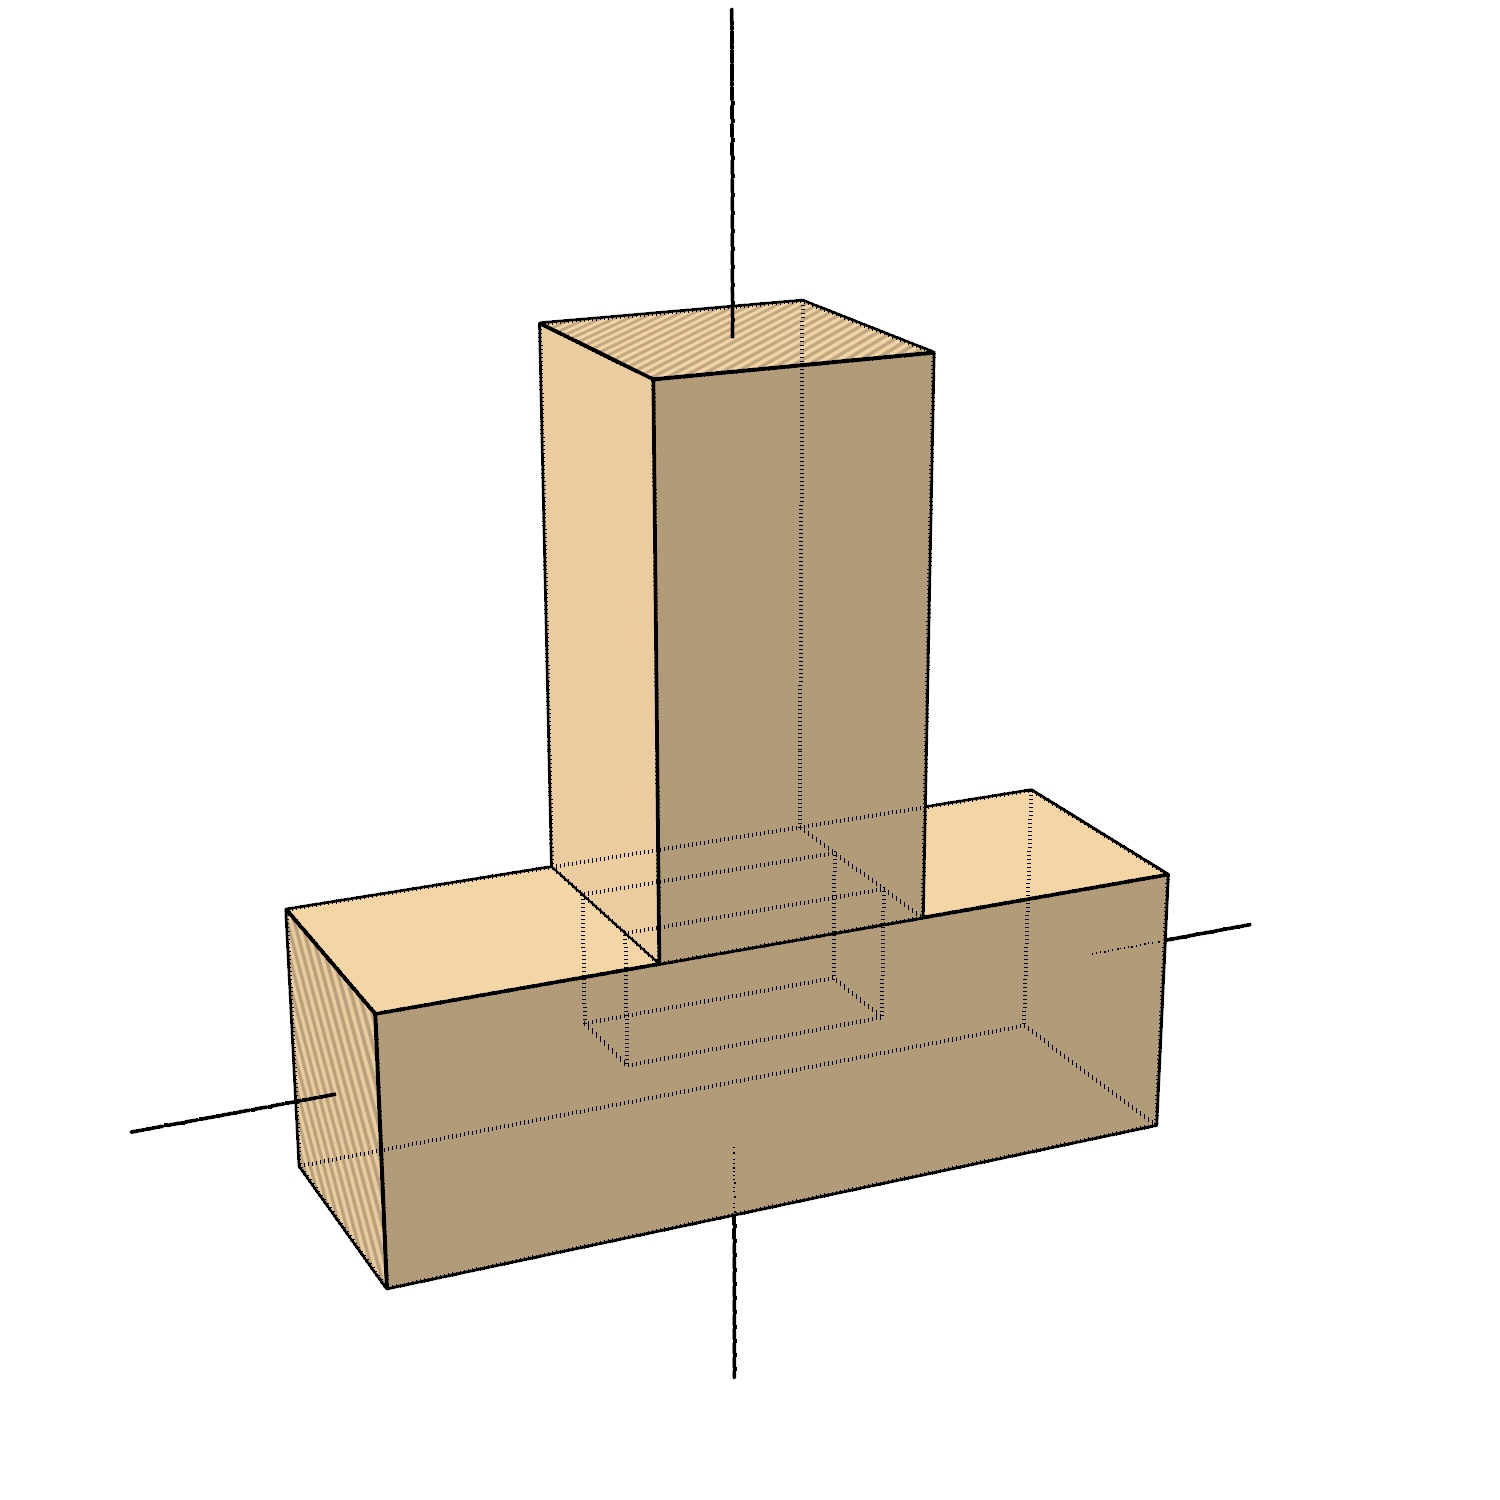
\includegraphics[width=\textwidth]{./images/image18.jpg}
\end{subfigure}
\hfill
\begin{subfigure}[b]{0.18\textwidth}
\centering
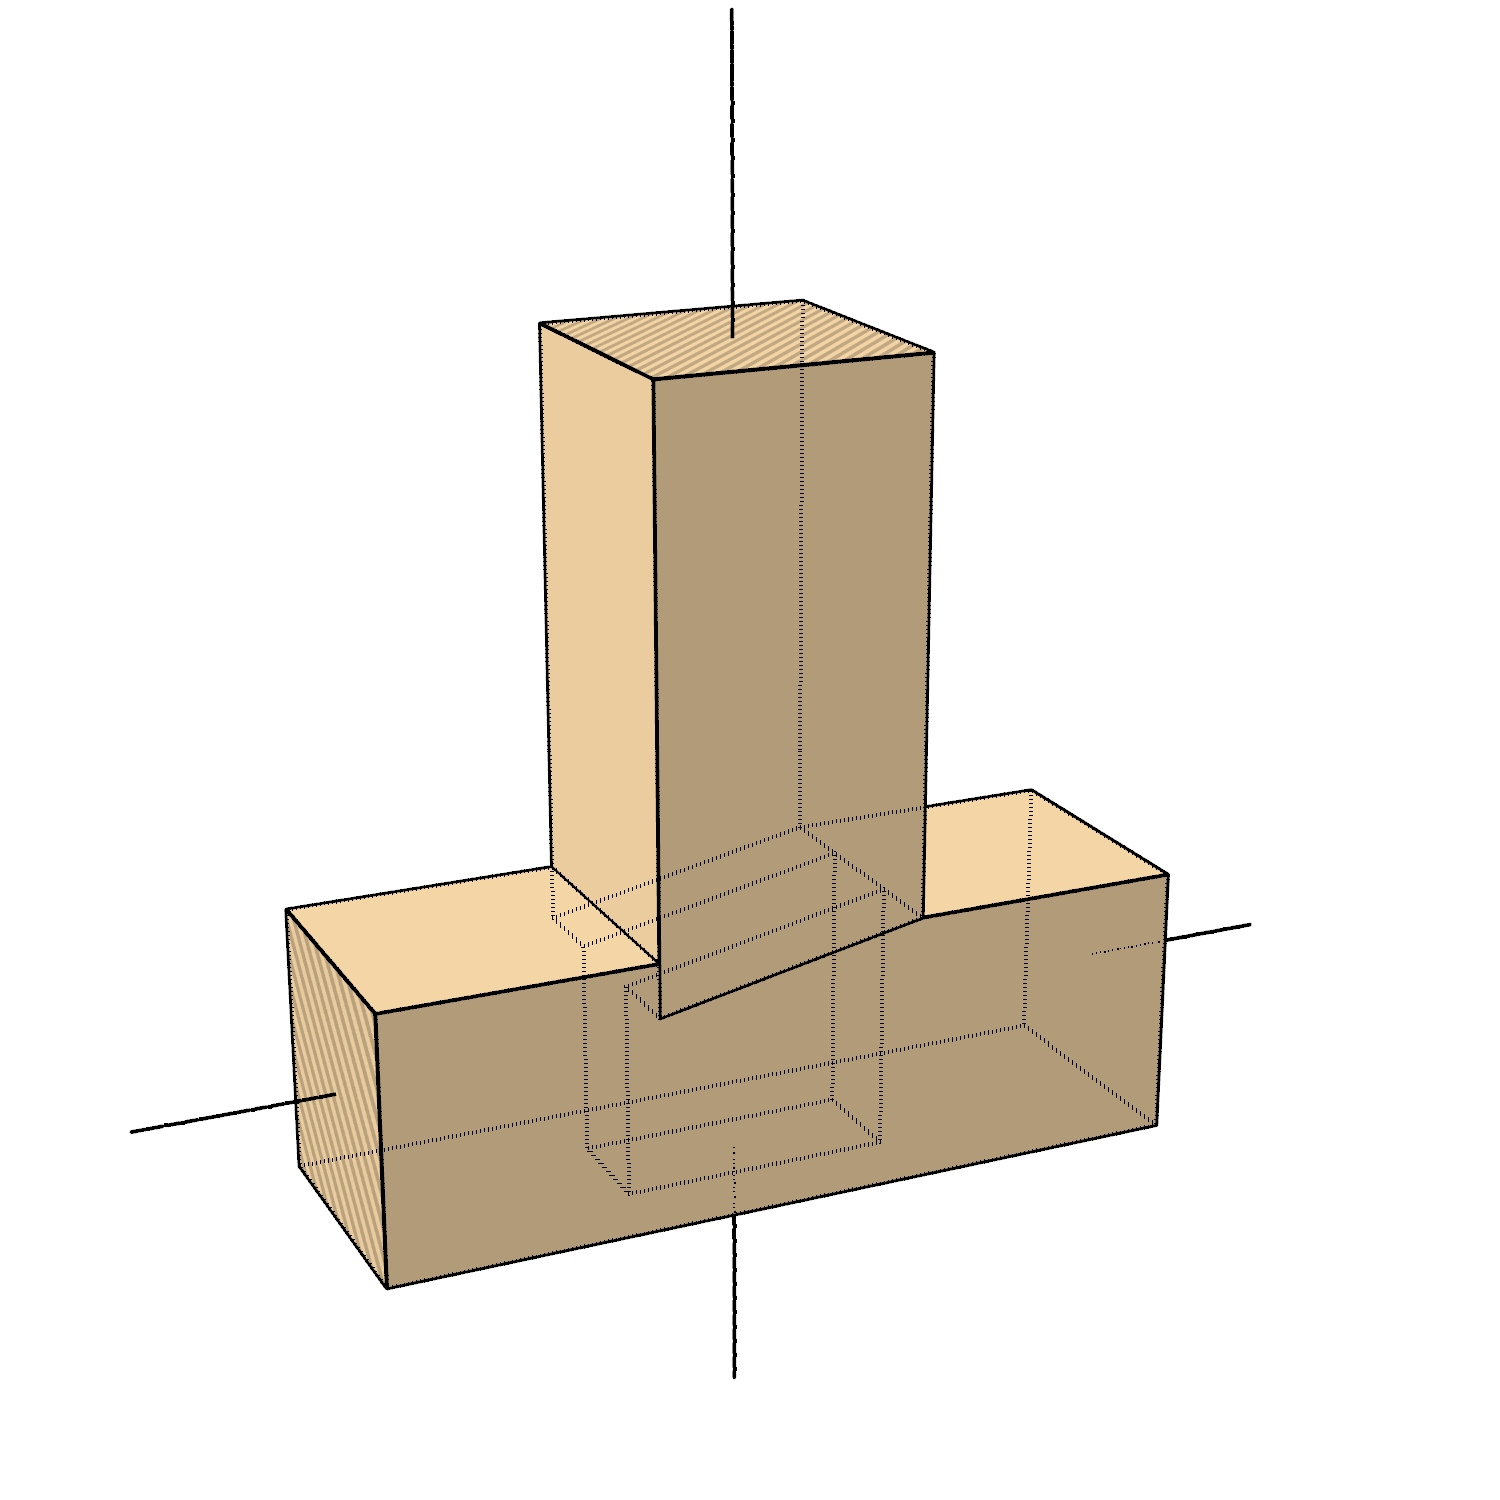
\includegraphics[width=\textwidth]{./images/image4.jpg}
\end{subfigure}
\end{figure}


Different ways to parametrise a joint model can result in different behaviour during size and angle adaptations. The choice of parameterization affects not only the structural behaviour of the joint but also the range of which a joint model can deform before it becomes invalid. For example, an intersection angle adaptation may result in an undercut geometry that cannot be cut with an automatic joinery machine.

Therefore it is common to consider the fabrication process and its constraints when creating a parametric joint model \href{https://www.zotero.org/google-docs/?mr32kk}{(Vestartas, 2021)}. Some joint designs are even dependent on the shape of the cutting tool. For example, the dovetail joint in the images below (left) is created by a dovetail milling cutter (below image, right). In those scenarios, it is necessary to contact the fabricator for a list of possible joint feature dimensions. 

\begin{figure}[H]
\centering
\begin{subfigure}[b]{0.45\textwidth}
\centering
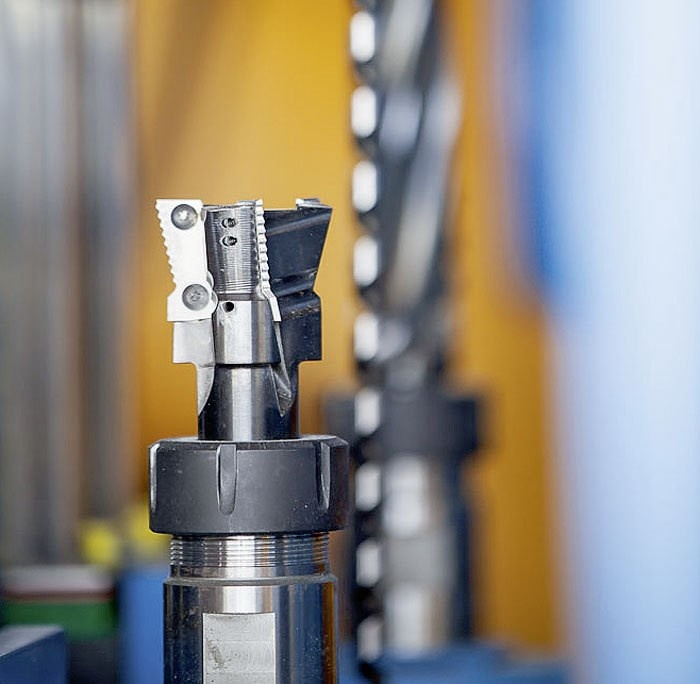
\includegraphics[width=\textwidth]{./images/image2.jpg}
\end{subfigure}
\hfill
\begin{subfigure}[b]{0.45\textwidth}
\centering
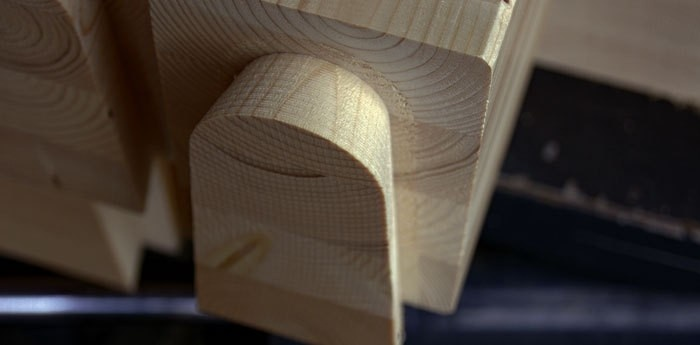
\includegraphics[width=\textwidth]{./images/image15.jpg}
\end{subfigure}
\end{figure}


{\footnotesize Photo by Hannes Plackner \href{https://www.zotero.org/google-docs/?ijZDtG}{(}\href{https://www.zotero.org/google-docs/?ijZDtG}{\textit{High-Tech Dovetails}\href{https://www.zotero.org/google-docs/?ijZDtG}{}, 2014)}}

\begin{flushleft}
Parametric joint models can be categorised according to what beam intersection topology it can adapt to. For example, side-side, side-end, and end-end types \href{https://www.zotero.org/google-docs/?SzXV4K}{(Vestartas $\&$ Weinand, 2020)}{\footnotesize .} This grouping allows automatic determination of what parametric model can be used for a given beam intersection type. In addition, the grouping can also include the assembly direction of the beams relative to each other. For example, the images below show assembly direction (red) being perpendicular to the beam axis (a and b) and parallel to the beam axis (c).
\end{flushleft}


\begin{flushleft}
{\footnotesize a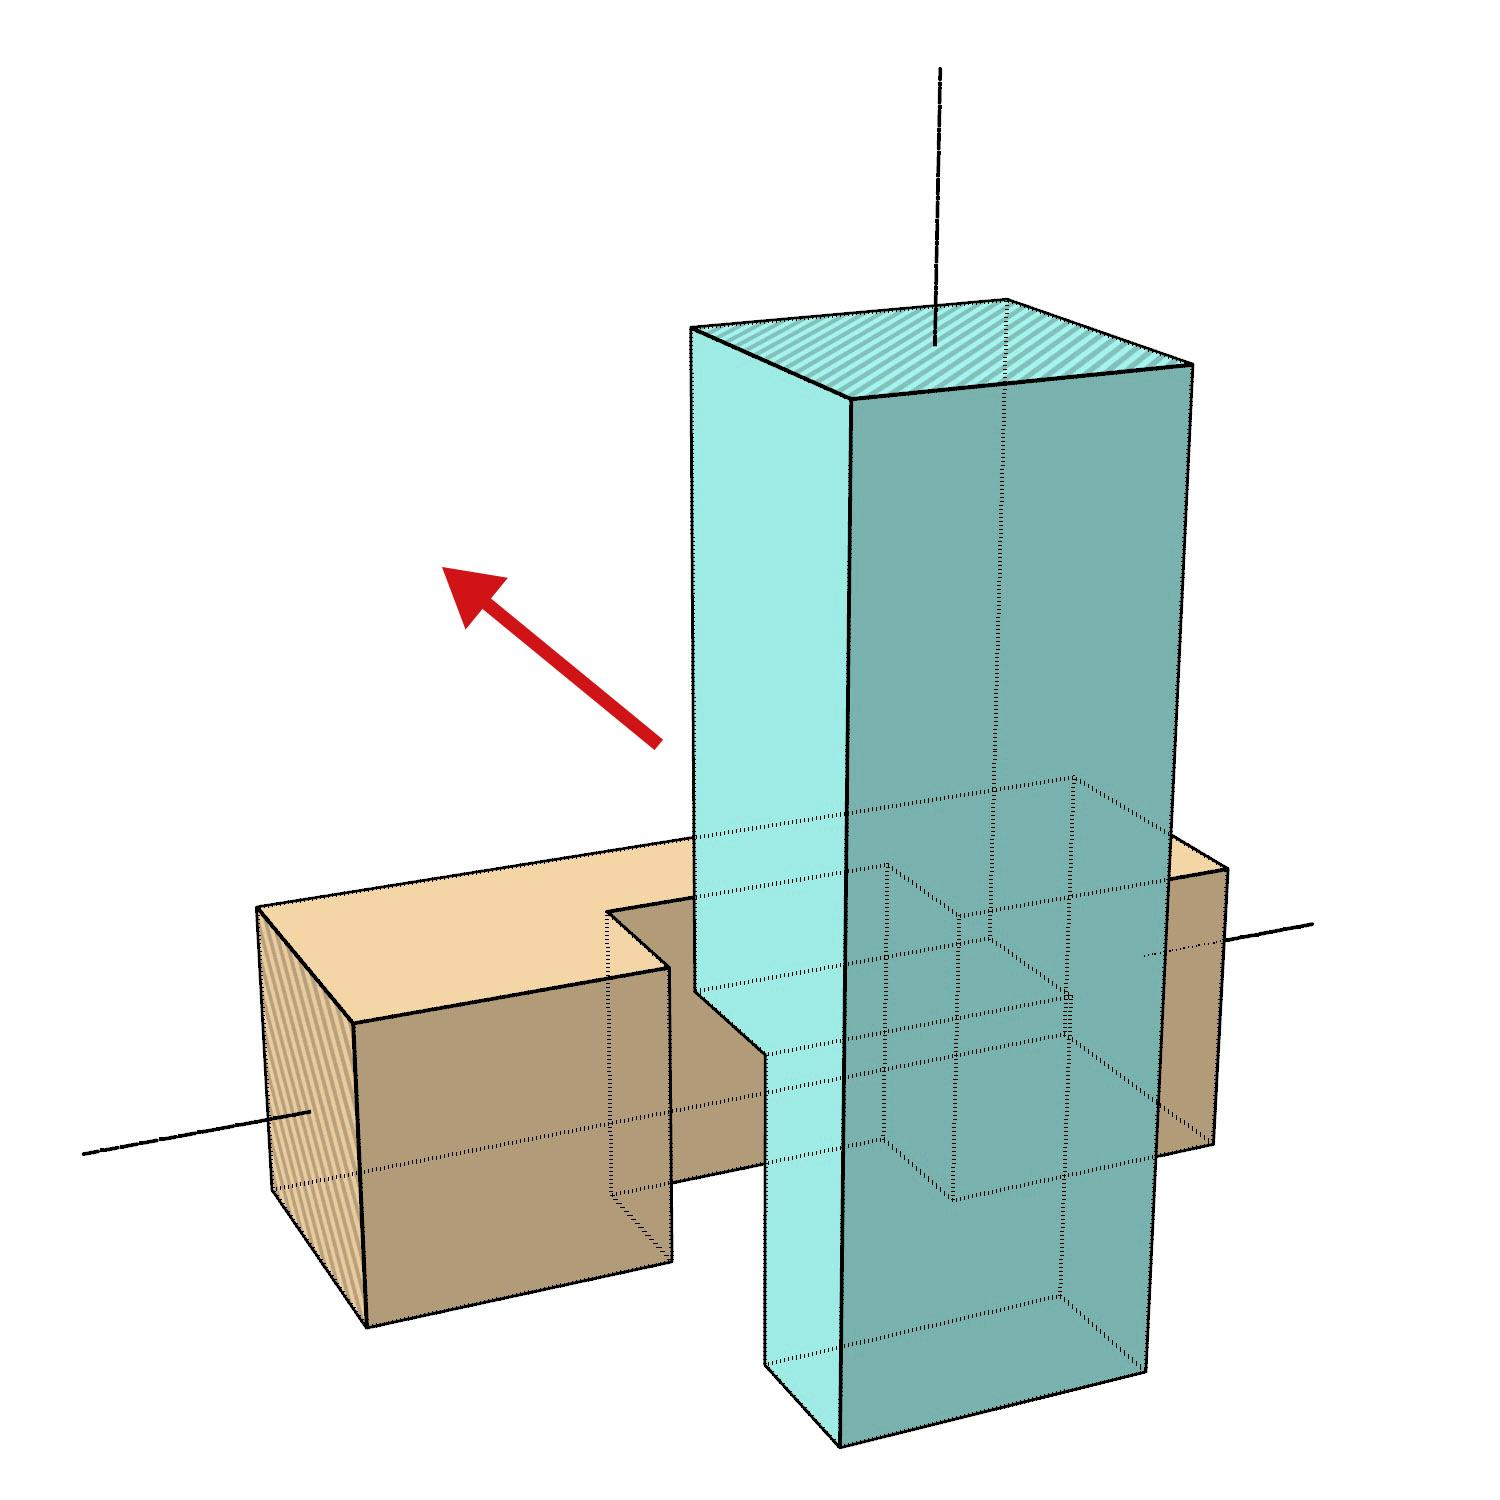
\includegraphics[width=5.0cm,height=5.0cm]{./images/image21.jpg}b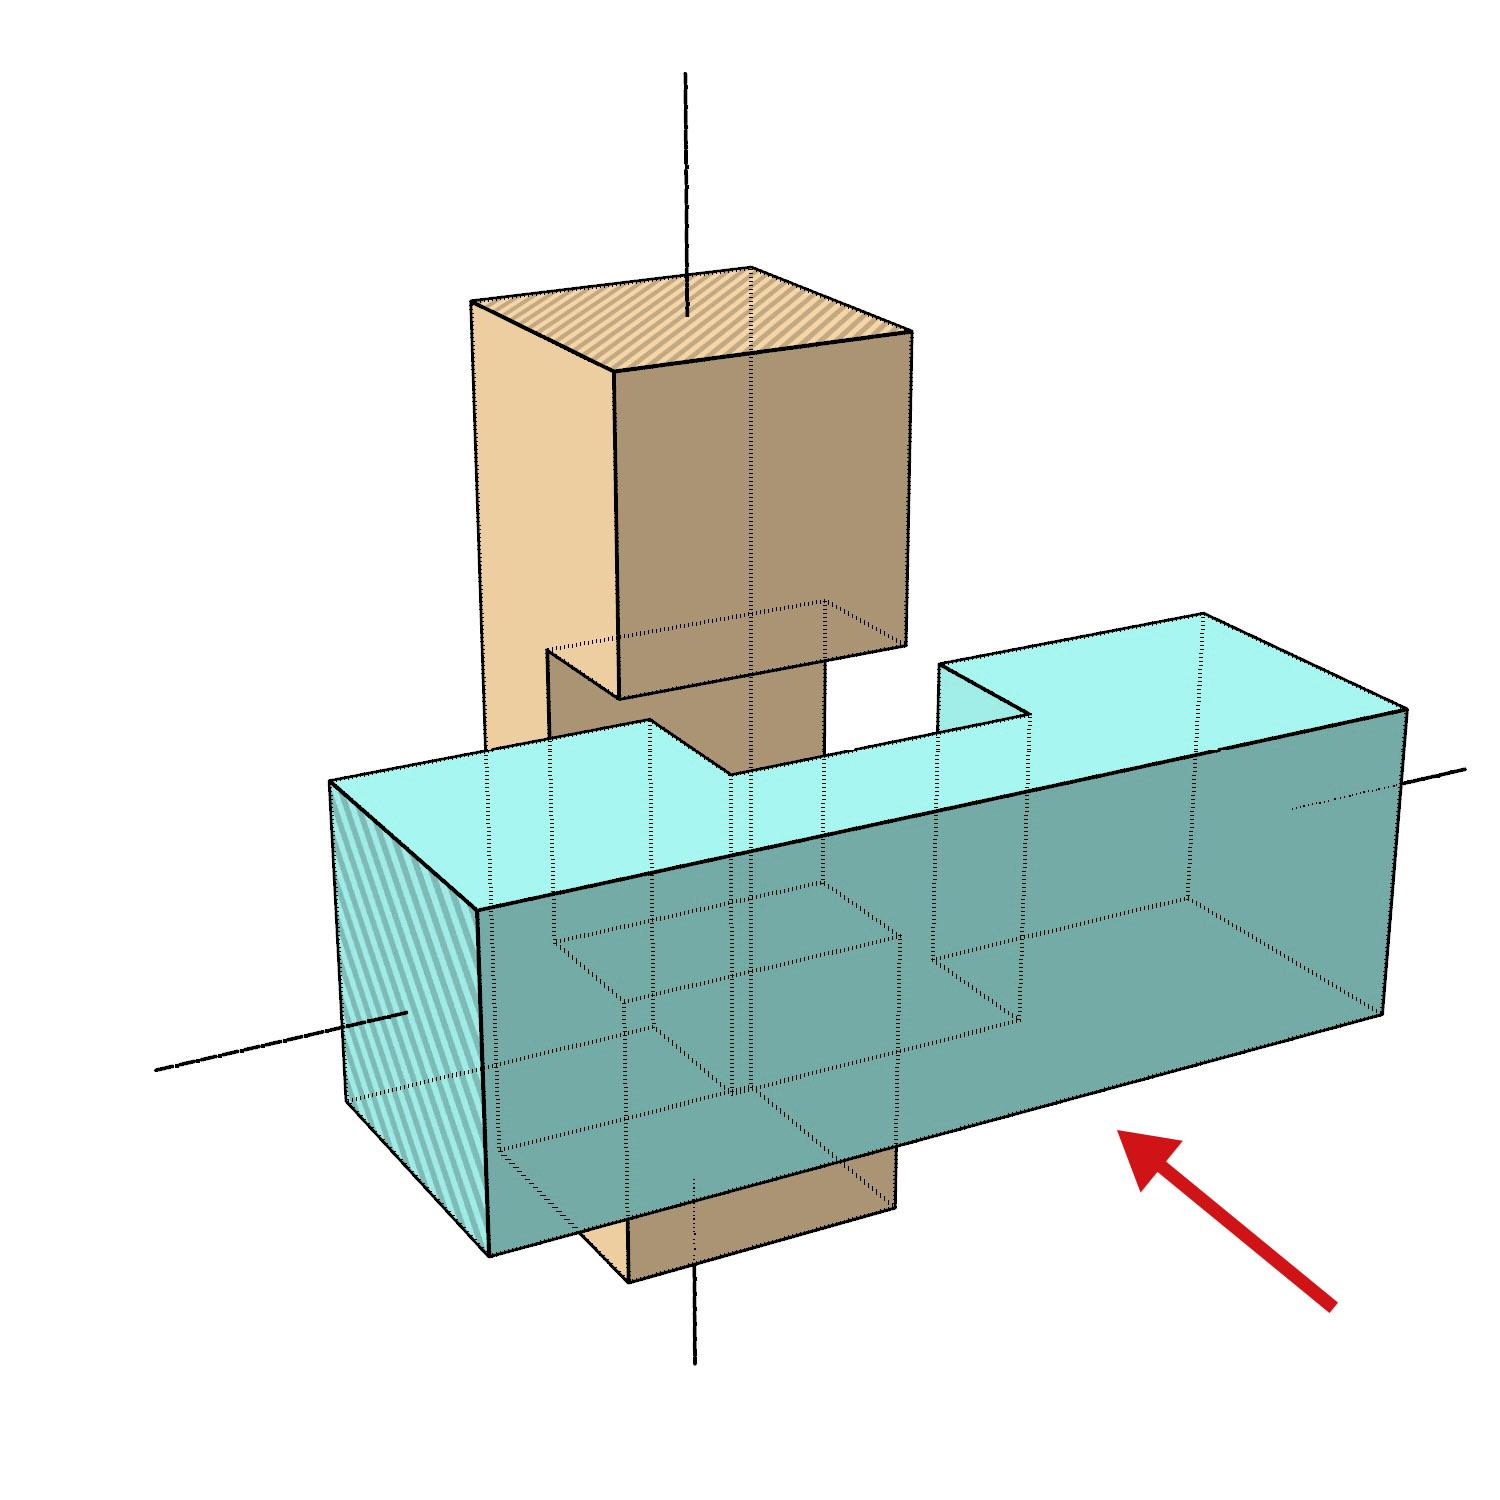
\includegraphics[width=5.0cm,height=5.0cm]{./images/image22.jpg}c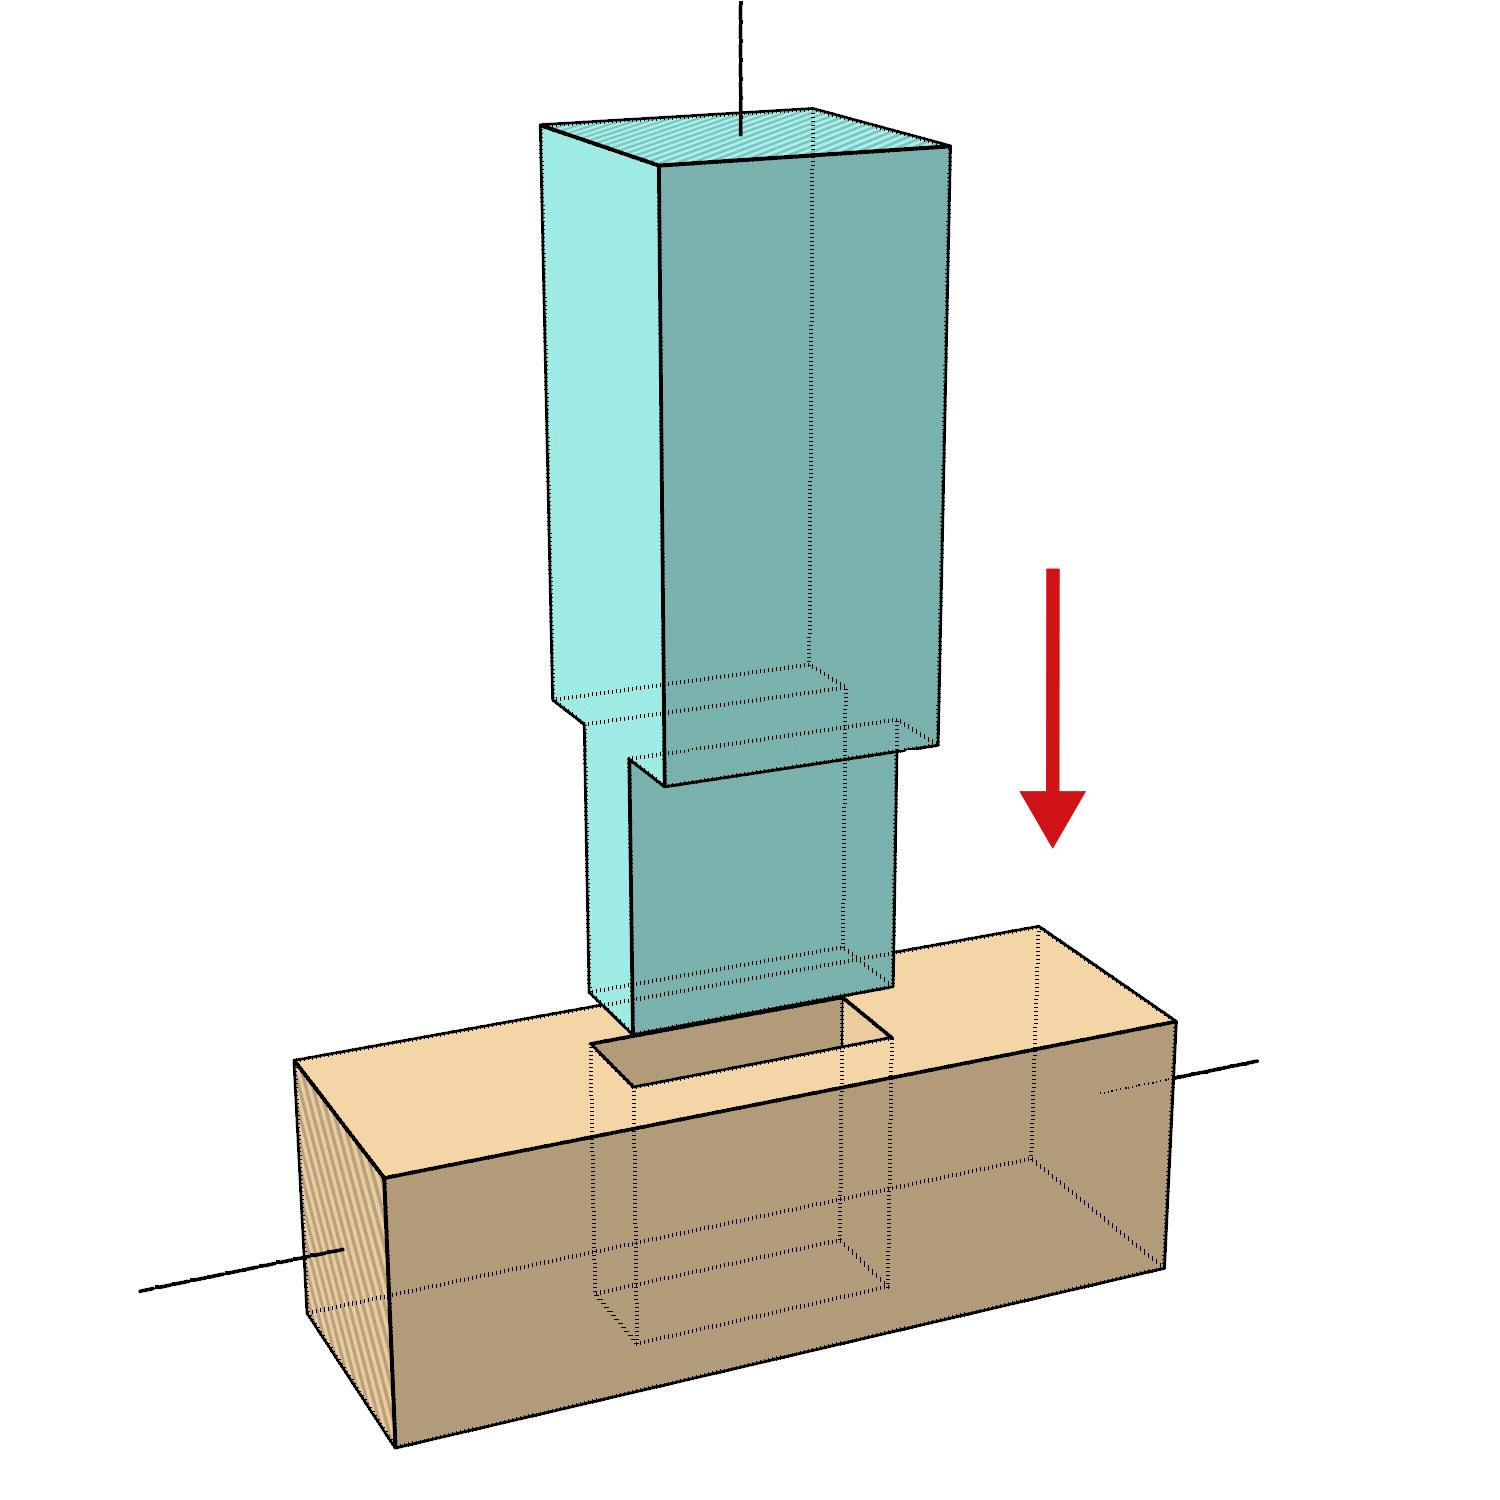
\includegraphics[width=5.0cm,height=5.0cm]{./images/image20.jpg}}
\end{flushleft}


It is worth noting that the solution space for a timber joint is large, and there are no existing approaches for evaluating all these requirements. Therefore, even though the solving process can theoretically be automatic, in practice, it often starts with the designer’s intuition and is later checked by the various design checks mentioned before. 

While the automatic modelling of timber joints is not an essential requirement for automatic assembly, it is important for a parametric design process. Even in a simple structure, there are many joints involved. The sheer number of joints makes the process tedious and prone to human error if they are modelled manually. Furthermore, the inclusion of assembly direction in a parametric joint model allows automatic design check for assemblability. It can also be used for generating the robotic assembly program, because the assembly direction defines one of the important movement targets for that specific beam. 

\subsection{User Interface for Fabrication Aware Design}

Creating designs in a highly constrained environment is often a balance between finding interesting possibilities while pushing the design boundary. Considering the many constraints, introduced in the previous sections, that are relevant to a robotically assembled timber frame structure, it is not hard to imagine the complexity of the design process. 

The computational approach to address these highly constrained problems is to use a powerful computer to search for valid solutions that could satisfy the given boundary conditions \href{https://www.zotero.org/google-docs/?IhApCE}{(Pottmann, 2013; Tam et al., 2018)}. In theory, as long as a constraint can be committed to computer code, it can be evaluated automatically. However, this technique is only meaningful for problems where the design space and the constraints are well defined \href{https://www.zotero.org/google-docs/?5kfhGC}{(Huang et al., 2016)}. In the case of architectural design, where the design space is infinite and the aesthetics of the structure is impossible to codify, the total exclusion of a designer is not meaningful. 

The alternative is a human-computer collaborative design process, or computer-aided design (CAD) in its essence, to combine the best of both agents. In this case, the human-computer interface (HCI), in the form of a graphical-user interface (GUI), becomes critical for successful collaboration of the two \href{https://www.zotero.org/google-docs/?3vtUPQ}{(Preece et al., 2015)}. 

The primary goal for such an interface is to provide designers with real-time feedback and guidance while allowing them to explore the design space and make informed decisions \href{https://www.zotero.org/google-docs/?5BPzBQ}{(Frich et al., 2019; Puentes $\&$ Ignacio, 2015)}. This involves visualising and communicating various constraints, warnings, and possible solutions through a well-designed interface that is both intuitive and user-friendly. To achieve this, the interface for designing a robotically-assemble timber structure should consider the following features: 

\begin{itemize}
	\item \textbf{Interactive 3D visualisation - }Enables navigation of the model over each assembly step for the human designer to understand temporal and spatial relationships between the beams, joints and robots.

	\item \textbf{Constraint visualisation - }Visualise constraint violations and fabrication limitations. 

	\item \textbf{Solution suggestions - }Offers ways to address constraint issues and improve the design.

	\item \textbf{Integrated robotic assembly planning -} Seamlessly incorporates assembly feasibility within the design environment.

	\item \textbf{Interactive parametric modelling workflow - }Facilitates quick iterations between different solutions when solving problems.

\end{itemize}
In summary, a user interface for fabrication-aware design should facilitate effective communication between the human designer and the computational tools, enabling a seamless and efficient design process. 

\section{Research Questions}

The challenges elaborated in the previous sections have indicated the highly interdisciplinary nature of this research. It includes the field of timber frame design, digital fabrication, machine design, computer graphics and robotics. Consequently, research questions that address these challenges require an integrated approach that combines expertise from these diverse fields..

Due to the novelty of the combination of the robotic assembly and integral timber joints, the thesis will adopt an exploratory research method (details in \textbf{Chapter 3 Methodology and Assumptions}). In this regard, the questions are open-ended and serve as a guide for exploration. 

\begin{enumerate}
	\item \textbf{What technologies (hardware and software) are required?}

\begin{enumerate}
	\item What are the \textbf{robotic end effectors} needed to assemble the joints? Can they be general purpose or specific to the type of joint being assembled?

	\item Is the \textbf{accuracy of a typical industrial robot }sufficient to assemble beams with joints? Is it necessary to develop \textbf{sense, alignment and compensation }methods to overcome misalignment?

	\item How suitable is an industrial robotic arm for performing spatial timber assembly? How can they be designed differently if they are optimised for construction purposes? How many robots are needed to assemble a building?

	\item How can \textbf{computational tools }support a robotic assembly process? Can \textbf{robotic programmes be generated automatically} based on assembly design?

\end{enumerate}
	\item \textbf{How will architectural design workflow and detailing have to change?}

\begin{enumerate}
	\item Will timber frame structures and integral timber joints be designed differently to accommodate the robotic process? For example, by adding \textbf{new details }to the beams and joints to \textbf{improve ease of assembly}? Can existing timber joinery machines produce these details?

	\item How will the design process be different with the added constraints of robotic assembly? How will \textbf{design validation }be performed?

	\item Who are the \textbf{new domain experts responsible for an automated construction process}? How can they participate in a design workflow?

\end{enumerate}
	\item What are the \textbf{possible implications if robots assemble timber buildings in the future?}

\begin{enumerate}
	\item Existing robots are generally not as agile as human workers. Will robotic assembly limit the \textbf{architectural and structural design possibilities}?

	\item How will \textbf{humans participate} in the transition to robotic construction? How will traditional roles such as carpenters change? What are the new roles that may emerge?

\end{enumerate}
\end{enumerate}

\newpage

\chapter{Methodology and Assumptions}

In this thesis, an exploratory research method was used. The first reason is the qualitative nature of the three research questions. The second reason is the novelty of the interdisciplinary topics which have yet to be studied in depth. The exploratory research consists of the following steps:

\begin{enumerate}
	\item \textbf{Identifying Challenges and Creating a Hypothetical Solution}– Although precedence works have already identified challenges in each subtopic \textit{(see \underline{Chapter 2.2 Computational and Design Challenges }and \underline{Chapter 2.1 Mechanical Challenges})}, a holistic analysis is still needed as certain challenges that are coupled together \textit{(see \underline{4.1.1 Addressing Assembly Challenges})}. This leads to a hypothetical robotic assembly process that is based on the idea of a robotic arm manipulating and collaborating with a set of robotic clamps \textit{(see \underline{4.1.2 Distributed Robotic Tool (DiRT) Approach})}.

	\item \textbf{Testing, observing and refining the Hypothetical Solution} – Technical development is performed, and their behaviour is observed with empirical experiments. A number of iterations is performed to refine the hypothetical robotic assembly process and to better understand the problems involved \textit{(see \underline{3.1 Research by Iterative Development})}.

	\item \textbf{Formulating relationships }– Critical analysis is performed during the development in each iteration and at the end of the thesis to answer the research questions and to provide possible avenues for future in-depth studies \textit{(see \underline{3.2 Epistemological assumptions})}.

\end{enumerate}
\section{Research by Iterative Development}

The most important part of this exploratory research is the emphasis on system development and hands-on empirical trial runs to refine the hypothetical solution for automatic assembly. Five distinct development rounds were conducted, each containing their own research goals, technical developments, experiments and observations \textit{(further elaboration in \underline{3.1.1 Setting Research Goals})}. The following flowchart summarises the iterative loops across the development rounds. 

\begin{figure}[H]
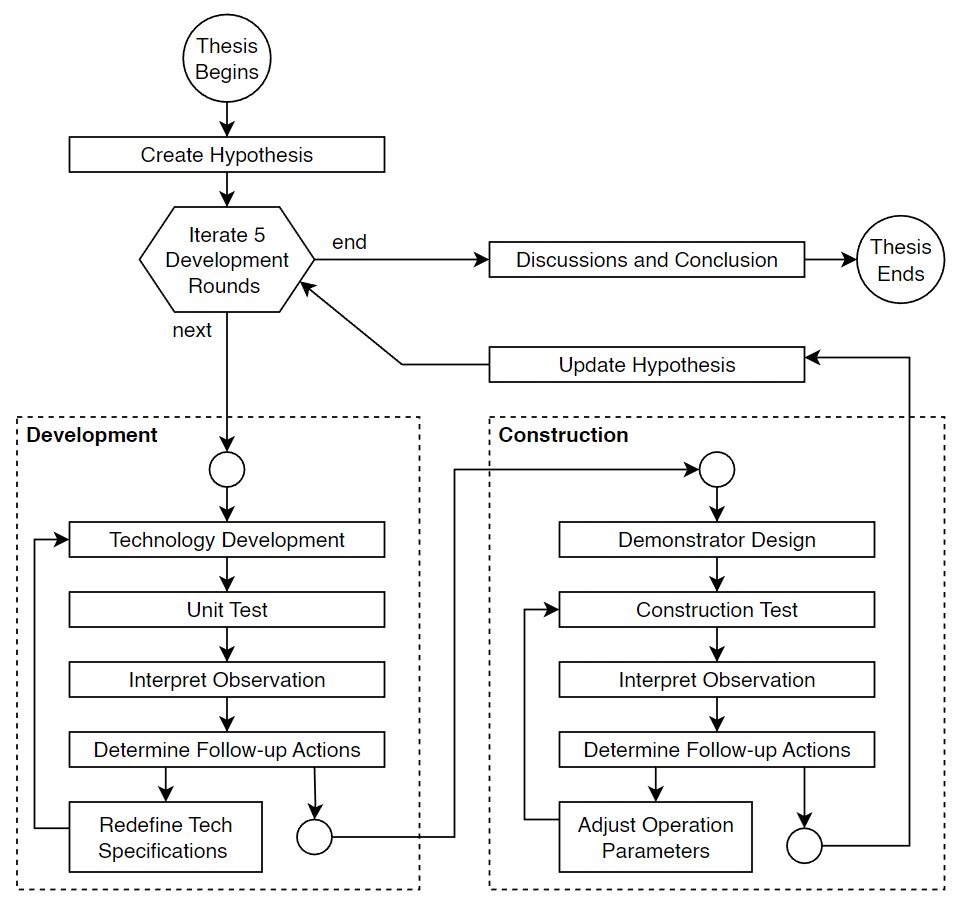
\includegraphics[width=15.92cm,height=14.96cm]{./images/image8.jpg}
\end{figure}


Within each \textbf{Development Phase}, small scale tests were performed and the technology was improved until it was ready for a full systematic test \textit{(further elaboration in \underline{3.1.2 Technical Development})}. 

The full full systematic test was performed by designing and constructing a \textbf{Demonstrator Structure} \textit{(further elaboration in \underline{3.1.3 Demonstrator Design})}. 

During the \textbf{Construction Phase}, certain adjustments of the process parameters are also possible. Afterwhich, the follow-up actions are determined for the next development round\textbf{ }\textit{(further elaboration in \underline{3.1.4 Observations and Interpretation})}.

\subsection{Setting Research Goals}

At the beginning of the first iteration, the goal was to design and prototype an assembly process and to test it with experiments. As new insights and discoveries are made, subsequent development iterations are guided by the discoveries and include follow-up explorations whenever necessary. Below is a summary of the goals in each phase:

\begin{itemize}
	\item \textbf{Development Round 1 - Clamp Prototype }– A minimal demonstration of the robotic clamp concept is developed to verify the process. The hardware being developed is only capable of assembling one type of lap joints with fixed dimensions. Nevertheless, it successfully performed the task and revealed opportunities for further improvements. \textit{(link to Chapter \underline{4 Dev Round 1 - Clamp Prototype)}}

	\item \textbf{Development Round 2 - Bus Stop Demonstrator }– The initial proof-of-concept clamp is redesigned to accommodate joints with different angles. Software is also developed to generate robot trajectory, control the robot arm, and control the robotic clamps wirelessly. Finally, a high level controller is developed to synchronise motion between the robotic arm and robotic clamps - an important aspect of the assembly process. The entire system was validated through the construction of a timber frame structure with 40 elements. \textit{(link to Chapter \underline{5 Dev Round 2 - Bus Stop Demonstrator)}}

	\item \textbf{Development Round 3 - Automatic Clamp Placement} - This phase completes the automation for mechanical tasks that are identified as low priority in the previous two phases. One of the highlights is the automatic placement and retrieval of robotic clamps on the structure. In addition, task planning and motion planning algorithms were introduced to study the automation of parsing designs to create robotic assembly programmes. The completed fully automatic assembly system was validated by reassembling the last demonstrator in a fully automatic manner.  \textit{(link to Chapter \underline{6 Dev Round 3 - Automatic Clamp Placement)}}

	\item \textbf{Development Round 4 - HyparHut Demonstrator} - This phase consists of a UI upgrade to improve interactive modelling in the CAD environment, the introduction of a fabrication-aware design workflow, and the introduction of a new robotic screwdriver. The new screwdriver allows the assembly of non-planar lap joints and can accommodate timber beams with different profile sizes. This vastly expands the design possibilities for timber frame structures that can be assembled by the automatic process. The new system was validated with the assembly of a structure with a hyperbolic paraboloid roof. One other highlight was the introduction of a vision based alignment process for improving the success rate for the robotic arm to pick up and place tools. \textit{(link to Chapter \underline{7 Dev Round 4 - HyparHut) }}

	\item \textbf{Development Round 5 - CantiBox Demonstrator} - By this round, the robotic assembly process had already achieved a high degree of automation and required little human intervention. The study was therefore expanded to integrate cutting-edge design methods with collaborators in two different fields. The first is structurally-informed joint design using novel design methods that is based on the theory of plasticity. This allows individually customised joints to respond to local load conditions. The main challenge on my part was to negotiate the intersection between assembly limitations, CNC machining limitations and structural optimization. The second is automated task and motion planning using PDDLStream to optimise redundant tasks and robotic motions. The main challenge is to formulate actions that can be understood by the computer algorithm to plan automatically. The combined technology was validated with the assembly of a structure with three modular boxes, each containing clamped and screwed joints. This also saw the largest amount of tools being used by the robotic assembly process, which provided insight for the future of the system. \textit{(link to Chapter \underline{8 Dev Round 5 - Cantibox)}}

\end{itemize}
\subsection{Technology Development}

The robotic assembly process required the development of novel hardware and software that form systems and subsystems that are interdependent in their operations. Below is an overview of the development categories showing their multidisciplinary nature. The software tools that are used for their development are listed in the bracket. 

\begin{itemize}
	\item \textbf{Mechatronics}

\begin{itemize}
	\item Robotic arm attachment hardware design (Rhinoceros 3D) 

	\item Robotic clamp and screwdriver hardware design (Rhinoceros 3D) 

	\item Robotic clamp and screwdriver electronics design (EAGLE)

	\item Other static hardware supporting construction (Rhinoceros 3D) 

\end{itemize}
	\item \textbf{Software for CAD}

\begin{itemize}
	\item CAD library for modelling timber parts and their assembly (Python)

	\item Design validation tools (Python)

	\item User Interface (UI) for interactive design modelling and validation (Python in Rhinoceros 3D) 

	\item CAM library for modelling robotic tools and their actions (Python)

\end{itemize}
	\item \textbf{Software for CAM}

\begin{itemize}
	\item Interface with task and motion planning software (Python) \textit{(footnote: in collaboration with YiJiang Huang)}

\end{itemize}
	\item \textbf{Software for control and execution}

\begin{itemize}
	\item Robotic clamp and screwdriver firmware (C++)

	\item Wireless communication firmware (C++)

	\item Robotic arm and robotic tools synchronisation controller (Python, ROS)

	\item Task execution and process monitoring software (Python)

\end{itemize}
\end{itemize}
During development, multiple technical solutions can often be used to achieve a particular goal. The principle for selecting a specific option included the following criteria: 

\begin{enumerate}
	\item The cost of implementation is reasonable in the architectural construction context, and testing costs can be afforded by the given research budget \textit{(see appendix about the budget)}.

	\item The implementation can be tested and observed within our laboratory.

	\item Software and hardware dependency is open source.

	\item The implementation is potentially generalisable. (e.g. a tool that can assemble more types of joints)

	\item The implementation is compatible with existing industrial practices or norms. (e.g. working with existing construction-grade tolerance instead of demanding a car-component-like accuracy) 

\end{enumerate}
Given the complexity of the AEC industry and its tendency to resist systematic changes, these principles guided the research direction towards finding implementable solutions with high impact.

\subsection{Demonstrator Design}

At the end of development phase 2, 4 and 5, the developed assembly process was observed and evaluated by the construction of a prototype structure. This is often called a demonstrator in the field of digital fabrication research. In total, there were three real-scale (1-to-1) demonstrators designed for this thesis. For the purpose of technical evaluation, the use of real-scale experiments revealed issues that were otherwise not observable in a computer simulation or a small-scale test. From the perspective of architectural design, the demonstrators served as a design study that can be experienced in person. Because of the high material cost and long preparation time required to construct such a demonstrator, each of them serves multiple investigation purposes to maximise the knowledge that can be extracted. Below is a list of design guidelines used when designing the demonstrators:

\begin{enumerate}
	\item The structure can be constructed with the developed system.

	\item The structure fits within our laboratory.

	\item The structure can demonstrate the flexibility of the assembly system (e.g. different types of joints, different joint angles, different element sizes, and different numbers of elements).

	\item The structures should present various difficulties for the assembly system (e.g. assembling very long elements, reaching into a congested space, joints very close to the ground or very high, many simultaneously assembled joints).

	\item The structures should contain various types of load-bearing elements (e.g. columns, floor beams, joists, diagonal bracings, rafters).

\end{enumerate}
During the design and preparation of the demonstrator, the newly developed CAD software (data structures, algorithms and user interfaces) was observed when it was used to model and encode the design. Flexibility and usability was observed first hand by the author, and improvements are sometimes implemented within the same development phase. The CAM software for translating design to robotic trajectories and execution programs was also tested. The result of this software is validated by performing digital checks such as robot kinematic simulation to catch collision problems. These problems must be fixed before the design phase can be concluded and timber parts can be ordered from the fabricator. 

During the demonstrator construction (also called Robotic Execution), the mechatronics hardware and control software was observed. The observation includes the dynamic behaviour when assembling different joint geometry and beam sizes at different orientations and with different support conditions. These observations provided evidence to identify key factors that limit system performance.  In addition, real world effects (such as gravity, material and robot inaccuracy) were observed during the assembly process to better understand fabrication constraints. This was used to improve the accuracy of automatic design checks for the fabrication-aware workflow.

Finally, the productivity of the robotic process was also observed by studying the time distribution during execution. While the exact duration in a laboratory condition may not correspond to an industrial automation scenario, it can reveal process bottlenecks and suggest possible improvements. Finally, unplanned manual interventions, such as robotic collisions, and overload errors due to jamming, are recorded and analysed qualitatively to identify patterns.

The timber parts used for the demonstrators were ordered from an industrial timber fabricator. Ordering from industry was preferred over creating the components within our laboratories because it allows a reality check of whether the newly developed digital workflow and timber details are compatible with the existing upstream industry. We have identified a single company (Auer Holzbau, Switzerland) to provide all the machining services in favour of consistency. The machining was performed on a recently released automatic joinery machine model (ROBOT-Drive 1250) manufactured by Hans Hundegger AG, Germany. The transfer of timber geometrical data is based on a proprietary file format of Cadwork (version 28). This is because the timber machining industry in Switzerland accepts it as a de facto standard for contractual agreement on the geometry of parts.

\subsection{Observations and Interpretation}

The \textbf{observations }made during the preparation and the execution of the demonstrators are documented as objectively as possible for each development phase (from Chapters 6 to 10). Based on these observations, \textbf{interpretations }are made to explain success and failure and are subsequently used to determine \textbf{follow-up actions}. Readers should be aware of the possible subjectivity in the interpretations and follow-up actions \textit{(See \underline{3.2 Epistemological assumptions} and \underline{3.3 Axiological assumptions})}. 

\begin{figure}[H]
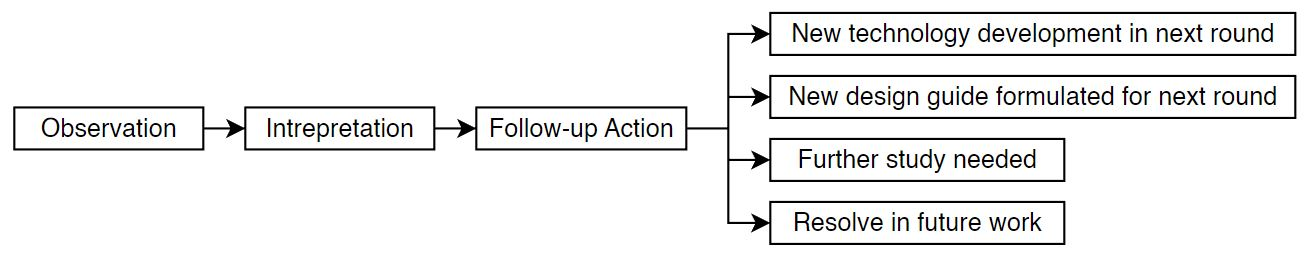
\includegraphics[width=15.92cm,height=3.17cm]{./images/image10.jpg}
\end{figure}


The diagram above shows different types of follow-up actions. For example, an observation may suggest new technology developments to improve the robotic assembly system. In some cases, further studies may be necessary to verify a causal relationship where the interpretations may be inconclusive. This can be caused by the scarcity of observations or the lack of scientific controls. Some other problems may require a design solution rather than a technological one, which can be addressed by formulating design guidelines or by creating automatic design checks. 

Note that some of the follow-up actions, such as adjusting software and tuning operation parameters, can be performed within the same development round. On the other hand, during the construction phase, the prefabricated timber parts cannot be modified easily and issues related to the demonstrator design can only be addressed in the next iteration. In addition, mechatronic and hardware issues often require substantially longer time to resolve. These problems were mostly addressed in the next round. 

Finally, follow-up actions are implemented wherever appropriate as long as my skills, research time and budget allow. Otherwise, the problems are elaborated for future investigations. 

\section{Epistemological assumptions}

The aim of the research is to create knowledge by developing, integrating and observing the effects of various technologies and the decisions made when designing the demonstration structure.

\textbf{Success and Failure} were evaluated based on whether the observed technology supports the vision of automatic design-to-assembly for timber frame structures. While some of the evaluation metrics are quantitative, others are qualitative such as when studying the generalizability and limitations of a particular technology.

\textbf{Causal Relationships} were established by logical reasoning, discussion with domain experts (e.g. CNC operator, Robot Technician, Structural Engineer, Architect) or quantitative experiments (e.g. tuning operation parameters, substituting parts or subsystems). The specific method to identify relationships was selected individually depending on the nature of the inquiry.

\section{Axiological assumptions}

This thesis followed interpretivism principles, and many of this research's components are qualitatively analysed. Readers should therefore be aware of the author’s (my) background and its potential influence on the interpretation of data. In the rest of the thesis, first-person pronouns (i.e. I, my) are used as an indication of when decisions and interpretations are likely to be influenced by my background. Passive voice will continue to be used to describe objective observations and when making qualitative analyses.

\subsection{Researcher Background}

I was trained at the undergraduate and graduate levels as an architectural designer specialising in computational design. I have also practised mechatronics design in art and design, albeit without formal training. These experiences greatly influence my characterisation of the research questions as a technology development problem focusing on mechatronics and computational design instead of other pathways. For example, another researcher with a timber engineering background may approach the problem by proposing novel wood joints, or a roboticist may propose a novel control method for robotic manipulators. Nevertheless, mechatronics and computational design are the most common approach taken by many recent research projects, as introduced in the previous chapters.

\subsection{Laboratory Context}

The research is conducted in the Robotic Fabrication Lab (RFL) of the Institute of Technology in Architecture (ITA) at the Department of Architecture of ETH Zurich, where four industrial robotic arms are mounted upside-down on two gantry robots (custom design by Güdel Group AG, Switzerland), forming a robotic manipulator that covers a large space\textit{ (see \underline{5.2.2 RFL Robotic Platform for technical details})}. Each robot consists of six articulated joints, an independent vertical linear axis, and two horizontal linear axes on the gantry coupled with neighbouring robots. If only a single robot is concerned, all nine axes can be commanded to move synchronously. This offers kinematic redundancy that allows the robot body to avoid obstacles in dense environments. For this thesis, the robotic manipulator in the RFL represents a hypothetical robotic manipulator that acted as a testbed for developing the robotic assembly process. This also carries the assumption that lessons learnt from this setup can be extrapolated to on-site setups in the future. The details of this extrapolation are further discussed in the conclusion chapter \textit{(see \underline{11.2.1 Extrapolation to On-Site Robotic Systems})}. 

Our laboratory is also the home to many timber assembly research projects introduced in the context. This undoubtedly influences the research as existing robotic components and software infrastructure are adopted from previous research. For example, the choice of the automatic robotic quick-change system was the result of a donation from previous projects \textit{(see \underline{5.3.5 Docking adapter})}. Another example is the choice of online robot control middleware \textit{(see \underline{5.2.4 Distributed Control System})}, which was determined by our laboratory's standard mode of operations.

\subsection{Participants in User Interface Study}

While the user interface consists of only a small portion of the development work, it is interesting to observe how designers can use the newly developed design interface. In order to gather a bigger picture, participants (other than myself) are invited to design two of the three demonstrators. During the design sessions, which often span multiple weeks, I offered technical guidance to the designer and observed what knowledge I explicitly communicated to the participant. This mitigates some of my subjectivity when considering implicit versus explicit knowledge, especially because I am the main developer of both software and hardware systems. 

\section{Collaborations}

Throughout this thesis, I collaborated with domain experts for some technological developments outside of my skills and knowledge. Their expert knowledge about state of the art in their respective fields helped me formulate the initial hypothetical solution. 

\begin{itemize}
	\item \textbf{Structural Analysis and Timber Joint Design }problems were advised by Dr. Davide Tanadini (Chair of Structural Design, ETH Zurich). His research focuses on possible applications of the theory of plasticity and graphic statics on timber structures and joints and their implementation in digital fabrication. In particular, the last demonstrator was designed by a student under his supervision (global design) and the joints were customised by the models and software he developed as part of this thesis. His PhD dissertation is titled ``Limit analysis and timber plasticity. Plastic design of interlocking timber-to-timber connections" \textit{(cite: Davides thesis) }Together with this thesis, they form part of the NCCR Digital Fabrication research project ‘Spatial Timber Assemblies’.

	\item \textbf{Robotic Task and Motion Planning (TAMP) }problems were advised by Dr. Yijiang Huang (Digital Structures Research Group, MIT, USA). His introduction and advice to the field was essential for me to understand the nature of the complicated problems involved. We worked in close collaboration for realising the three demonstrators, which led to the discovery of many new techniques to bridge between the highly technical fields (robotics and computer algorithms) and architectural design. Many of the planning related software, including all of the motion planning backend were developed by him. His PhD dissertation is titled ``Algorithmic planning for robotic assembly of building structures," \href{https://www.zotero.org/google-docs/?GiBuSm}{(Huang, 2022)}. Both of our researches share the same vision towards improving automation from design to assembly. 

	\item \textbf{Machine Design and Construction}, especially the later development with the screwdriver were advised by Prof. Dr. Agathe Koller and Marco Rossi (both from The Institute for Lab Automation and Mechatronics ILT, OST, Switzerland). They were directly involved in the conceptualization of the screwdriver operation mechanism and the innovative pin gripper mechanism. Marco also offered valuable instructions for machine design and construction, made some of the hardware parts and advised on the tests during hardware development

\end{itemize}
\section{Thematic Reading Guide}

The following five chapters (chapter 4 to 8) are written in chronological order corresponding to five development rounds. This is important for understanding the exploration as an evolution between experiments and observations.  Each chapter contains the following sections:

\vspace{1\baselineskip}
\begin{itemize}
	\item \textbf{Goal - }Identify the goal and scope for the entire development round

	\item \textbf{Background }- Background knowledge needed to understand the rationale for some of the development.

	\item \textbf{Development }- Technical description of the developed hardware and software. Some topics include the tests that were performed during development.

	\item \textbf{Lesson Learnt - }Observations, findings and interpretations related to the robotic construction demonstration. Some topics include hypotheses of possible cause(s), possible solution(s) and the follow-up action(s) taken. 

Readers who are interested only in a specific theme may find the following guide helpful for identifying a specific section. Note that this list is not exhaustive. 

	\item \textbf{Distribute Robotic Tools (DiRT) assembly method}

\begin{itemize}
	\item \textbf{Initial working hypothesis} of the DiRT clamps assembly method (4.1.4 DiRT Clamping Assembly Process Task List (v1))

	\item \textbf{Operation method revised} after initial test (6.1.1 DiRT Clamping Assembly Process Task List (v2))

	\item \textbf{Operation method with screwdrivers} (7.3.20 Flowchart for Screwdriver Assembly)

	\item \textbf{Operation method with clamps and screwdrivers }(8.1.1 Combined Operation of Clamps and Screwdrivers)

	\item \textbf{Generalised operation principle} (10.3 Generalised DiRT system)

\end{itemize}
	\item \textbf{Two Types of DiRT Assembly Tools}

\begin{itemize}
	\item \textbf{Clamp }for planar lap joints

\begin{itemize}
	\item Hardware (5.3.4 Lap Clamp CL3 Hardware)

	\item Electronics (5.3.6 CL3 Clamp Electronics)

	\item Firmware (5.3.8 CL3 Firmware)

\end{itemize}
	\item \textbf{Screwdriver }for planar and non-planar lap joints 

\begin{itemize}
	\item Hardware (7.3.7 Lap Screwdriver SL1 and SL1\_G200 Hardware)

	\item Electronics (7.3.11 SL1 Screwdriver Electronics)

	\item Firmware (7.3.12 Screwdriver Firmware (L1 Control))

\end{itemize}
\end{itemize}
	\item \textbf{Other DiRT supporting hardware}

\begin{itemize}
	\item \textbf{Radio }(5.3.9 Radio Network)

	\item \textbf{Gripper }

\begin{itemize}
	\item Short Parallel Gripper (5.3.5 Parallel Gripper PG500 and PG1000)

	\item Long Parallel Gripper (7.3.8 Parallel Gripper PG1500 for Long Beams)

	\item Pin Gripper on Screwdriver (7.3.5 Pin Gripper Mechanism)

\end{itemize}
	\item \textbf{Docking Adapter}

\begin{itemize}
	\item 7.3.9 Docking Adapter Lock Sensor

\end{itemize}
	\item \textbf{Camera Alignment System}

\begin{itemize}
	\item 7.3.14 Camera-Marker Alignment Correction System

	\item 7.3.15 Camera-Marker Hardware on Docking Adapter

	\item 8.3.4 Camera-Marker Hardware on CL3 Clamp

	\item 7.5.2.5 Visual-guided Docking Process

\end{itemize}
\end{itemize}
	\item \textbf{Design Software and Workflow}

\begin{itemize}
	\item \textbf{Design and Modeling Frontend}

\begin{itemize}
	\item \textbf{Design UI in Rhino Grasshopper} (5.3.13 CAD / CAM User Interface)

	\item \textbf{Design UI (revised) in Rhino Python }(6.3.3 Design Software Implementation in Rhino Python)

	\item \textbf{Process Design Visualization} (6.3.4.6 Process Visualization and Adjustment)

\end{itemize}
	\item \textbf{Backend}

\begin{itemize}
	\item \textbf{Assembly Model} (5.3.12 Assembly Model Data Structure and Functions)

	\item \textbf{Process Model} (6.3.4 Process Design Workflow)

\end{itemize}
	\item \textbf{Conceptual}

\begin{itemize}
	\item 7.1.1 Deformation-Awareness and Error Correction by Triangulation)

	\item 7.5.2.6 Global Correction Approach

\end{itemize}
\end{itemize}
\end{itemize}
\vspace{1\baselineskip}
\begin{itemize}
	\item \textbf{Task and Motion Planning }workflow (6.3.4 Process Design Workflow)

\begin{itemize}
	\item \textbf{Narrow Passage Problem }(5.5.3 Narrow Passage Problem)

	\item \textbf{Fast Check by IK} (7.3.21 Fast Design Validation with IK Check)

	\item \textbf{Fast Check by LMG Planning} (7.3.22 Planning Order by Motion Group)

	\item \textbf{Non-sequential MMMP Solver} (6.3.6 Non-Sequential Planning Order)

\end{itemize}
	\item \textbf{Three Demonstration Structures Constructed}

\begin{itemize}
	\item \textbf{BusStop }Pavilion (5.4.4 Demonstrator Design - BusStop Pavilion)

	\item \textbf{HyparHut }Pavilion (7.4.3 Demonstrator Design  - HyparHut Pavilion)

	\item \textbf{CantiBox }Pavilion (8.4.3 Demonstrator Design  - CantiBox Pavilion)

\end{itemize}
\end{itemize}

\end{document}